% The main file. It contains definitions of basic 
% parameters and includes all other parts.

%% Settings for single-side (simplex) printing
% Margins: left 40mm, right 25mm, top and bottom 25mm
% (but beware, LaTeX adds 1in implicitly)
\documentclass[12pt,a4paper]{report}
\setlength\textwidth{145mm}
\setlength\textheight{247mm}
\setlength\oddsidemargin{15mm}
\setlength\evensidemargin{15mm}
\setlength\topmargin{0mm}
\setlength\headsep{0mm}
\setlength\headheight{0mm}
% \openright makes the following text appear on a right-hand page
\let\openright=\clearpage 

%% Settings for two-sided (duplex) printing
% \documentclass[12pt,a4paper,twoside,openright]{report}
% \setlength\textwidth{145mm}
% \setlength\textheight{247mm}
% \setlength\oddsidemargin{14.2mm}
% \setlength\evensidemargin{0mm}
% \setlength\topmargin{0mm}
% \setlength\headsep{0mm}
% \setlength\headheight{0mm}
% \let\openright=\cleardoublepage

\usepackage{xcolor}

%% Generate PDF/A-2u
\usepackage[a-2u]{pdfx}

%% Character encoding: usually latin2, cp1250 or utf8:
\usepackage[utf8]{inputenc}

\usepackage[english]{babel}
%% Prefer Latin Modern fonts
\usepackage{lmodern}

%% Further useful packages (included in most LaTeX distributions)
\usepackage{amsmath}        % extensions for typesetting of math
\usepackage{amsfonts}       % math fonts
\usepackage{amsthm}         % theorems, definitions, etc.
\usepackage{bbding}         % various symbols (squares, asterisks, scissors, ...)
\usepackage{bm}             % boldface symbols (\bm)
\usepackage{graphicx}       % embedding of pictures
\graphicspath{{img/}}
\usepackage{fancyvrb}       % improved verbatim environment
\usepackage{natbib}         % citation style AUTHOR (YEAR), or AUTHOR [NUMBER]
\usepackage[nottoc]{tocbibind} % makes sure that bibliography and the lists
			    % of figures/tables are included in the table
			    % of contents
\usepackage{dcolumn}        % improved alignment of table columns
\usepackage{booktabs}       % improved horizontal lines in tables
\usepackage{paralist}       % improved enumerate and itemize
\usepackage{xspace}
\usepackage{soul}
\usepackage{listings}
\usepackage{tcolorbox}
\usepackage{etoolbox}

% \usepackage[usenames]{xcolor}  % typesetting in color

\usepackage[acronym,toc]{glossaries} % making glossaries
\usepackage[normalem]{ulem} % tables
\usepackage[cache=false]{minted}

\definecolor{LightGray}{gray}{0.95}

%%JaKl comment macros - to be removed when cleaning the thesis
\newcommand{\TODO}[1]{{\color{red}{\textbf{TODO: {#1}}\xspace}}}
\newcommand{\CONSIDER}[1]{{\color{blue}{\textbf{CONSIDER: {#1}}\xspace}}}
%%End of JaKl comment macros

%%% Basic information on the thesis

% Thesis title in English (exactly as in the formal assignment)
\def\ThesisTitle{Decentralized Web-based Data Storage for LinkedPipes Applications using Solid}

% Author of the thesis
\def\ThesisAuthor{Altynbek Orumbayev}

% Year when the thesis is submitted
\def\YearSubmitted{2020}

% Name of the department or institute, where the work was officially assigned
% (according to the Organizational Structure of MFF UK in English,
% or a full name of a department outside MFF)
\def\Department{Department of Software Engineering}

% Is it a department (katedra), or an institute (ústav)?
\def\DeptType{Department}

% Thesis supervisor: name, surname and titles
\def\Supervisor{RNDr. Jakub Klímek, Ph.D.}

% Supervisor's department (again according to Organizational structure of MFF)
\def\SupervisorsDepartment{department}

% Study programme and specialization
\def\StudyProgramme{Computer Science}
\def\StudyBranch{Software and Data Engineering}

% An optional dedication: you can thank whomever you wish (your supervisor,
% consultant, a person who lent the software, etc.)
\def\Dedication{%
I want to dedicate this thesis to my family and their support and motivation. This work wouldn't have been possible without them. 

I am also grateful to my friends from the Faculty of Mathematics and Physics at Charles University. Esteban, Memduh, Abishek, Yigit, and Vinit, with whom we had a great two years of fruitful discussions.

Finally, I would like to thank my supervisor RNDr. Jakub Klímek, for his insightful guidance, support, and reviews.
}

% Abstract (recommended length around 80-200 words; this is not a copy of your thesis assignment!)
\def\Abstract{
The following thesis work is focused on developing a decentralized web-based storage solution based on \solid{} project for the LinkedPipes Applications platform and demonstrate the full benefits of decentralized storage and the \solid{} technology. The \solid{} project, started by Sir Tim Berners-Lee, is focused on decentralizing the World Wide Web and decoupling data from applications on the Internet. The results of the practical work satisfy all defined functional and non-functional requirements stated by the LinkedPipes Applications project. The results of the work are integrated into the LinkedPipes Applications platform as a set of several software libraries allowing interaction with Solid Servers.
}

% 3 to 5 keywords (recommended), each enclosed in curly braces
\def\Keywords{%
{solid, linked data, client, server, storage, web}
}

%% The hyperref package for clickable links in PDF and also for storing
%% metadata to PDF (including the table of contents).
%% Most settings are pre-set by the pdfx package.
\hypersetup{unicode}
\hypersetup{breaklinks=true}

% Definitions of macros (see description inside)
%%% This file contains definitions of various useful macros and environments %%%
%%% Please add more macros here instead of cluttering other files with them. %%%

%%% Minor tweaks of style

% These macros employ a little dirty trick to convince LaTeX to typeset
% chapter headings sanely, without lots of empty space above them.
% Feel free to ignore.
\makeatletter
\def\@makechapterhead#1{
  {\parindent \z@ \raggedright \normalfont
   \Huge\bfseries \thechapter. #1
   \par\nobreak
   \vskip 20\p@
}}
\def\@makeschapterhead#1{
  {\parindent \z@ \raggedright \normalfont
   \Huge\bfseries #1
   \par\nobreak
   \vskip 20\p@
}}
\makeatother

% This macro defines a chapter, which is not numbered, but is included
% in the table of contents.
\def\chapwithtoc#1{
\chapter*{#1}
\addcontentsline{toc}{chapter}{#1}
}

% Draw black "slugs" whenever a line overflows, so that we can spot it easily.
\overfullrule=1mm

%%% Macros for definitions, theorems, claims, examples, ... (requires amsthm package)

\theoremstyle{plain}
\newtheorem{thm}{Theorem}
\newtheorem{lemma}[thm]{Lemma}
\newtheorem{claim}[thm]{Claim}

\theoremstyle{plain}
\newtheorem{defn}{Definition}

\theoremstyle{remark}
\newtheorem*{cor}{Corollary}
\newtheorem*{rem}{Remark}
\newtheorem*{example}{Example}

%%% An environment for proofs

%%% FIXME %%% \newenvironment{proof}{
%%% FIXME %%%   \par\medskip\noindent
%%% FIXME %%%   \textit{Proof}.
%%% FIXME %%% }{
%%% FIXME %%% \newline
%%% FIXME %%% \rightline{$\square$}  % or \SquareCastShadowBottomRight from bbding package
%%% FIXME %%% }

%%% An environment for typesetting of program code and input/output
%%% of programs. (Requires the fancyvrb package -- fancy verbatim.)

\DefineVerbatimEnvironment{code}{Verbatim}{fontsize=\small, frame=single}

%%% The field of all real and natural numbers
\newcommand{\R}{\mathbb{R}}
\newcommand{\N}{\mathbb{N}}

%%% Useful operators for statistics and probability
\DeclareMathOperator{\pr}{\textsf{P}}
\DeclareMathOperator{\E}{\textsf{E}\,}
\DeclareMathOperator{\var}{\textrm{var}}
\DeclareMathOperator{\sd}{\textrm{sd}}

%%% Transposition of a vector/matrix
\newcommand{\T}[1]{#1^\top}

%%% Various math goodies
\newcommand{\goto}{\rightarrow}
\newcommand{\gotop}{\stackrel{P}{\longrightarrow}}
\newcommand{\maon}[1]{o(n^{#1})}
\newcommand{\abs}[1]{\left|{#1}\right|}
\newcommand{\dint}{\int_0^\tau\!\!\int_0^\tau}
\newcommand{\isqr}[1]{\frac{1}{\sqrt{#1}}}

%%% Various table goodies
\newcommand{\pulrad}[1]{\raisebox{1.5ex}[0pt]{#1}}
\newcommand{\mc}[1]{\multicolumn{1}{c}{#1}}

%%% Glossary macros 
\newcommand{\solid}{SOLID}
\newcommand{\lpa}{LinkedPipes Applications Storage}
\newcommand{\lpas}{LinkedPipes Applications Storage}


%% Load glossary
% % Acronyms 
\newacronym{API}{API}{Application Programming Interface}
\newacronym{ETL}{ETL}{Extract, Transform and Load}
\newacronym{IRI}{IRI}{Internationalized Resource Identifier}
\newacronym{URI}{URI}{Uniform Resource Identifier}
\newacronym{URL}{URL}{Uniform Resource Locator}
\newacronym{LPA}{LPA}{LinkedPipes Application}
\newacronym{RDF}{RDF}{ Resource Description Framework}
\newacronym{SPA}{SPA}{Single-page Application}
\newacronym{LDVM}{LDVM}{Linked Data Visualization Model}
\newacronym{LDMVi}{LDVMi}{Linked Data Visualization Model implementation}
\newacronym{TTL}{TTL}{Turtle (syntax)}
\newacronym{LODC}{LOD Cloud}{Linked Open Data Cloud}
\newacronym{SPARQL}{SPARQL}{SPARQL Protocol and RDF Query Language}
\newacronym{W3C}{W3C}{World Wide Web Consortium}
\newacronym{LOV}{LOV}{Linked Open Vocabularies}
\newacronym{DOM}{DOM}{Document Object Model}
\newacronym{SSL}{SSL}{Secure Sockets Layer }
\newacronym{TLS}{TLS}{Transport Layer Security}

% Terms/Definitions
\newglossaryentry{endpoint}
{
    name=Endpoint,
    description={An endpoint is one end of a communication channel}
}

\newglossaryentry{assistant}
{
    name=Assistant,
    description={Refers to the Linked Pipes Visualization Assistant, which allows users to create, configure and publish visualizations based on input data sets}
}

\newglossaryentry{datacube}
{
    name={Data cube},
    description={multi-dimensional array of values}
}

\newglossaryentry{data-descriptor}
{
    name={Data descriptor},
    description={An SPARQL ASK query associated with a visualizer that determines if an input data graph can be visualized in the corresponding visualizer}
}

\newglossaryentry{data-source}
{
    name={Data source},
    description={Refers to any source of data, such as an RDF file, CSV, database, etc}
 }

\newglossaryentry{linked-data}
{
    name={Linked Data},
    description={a method of publishing structured data so that it can be interlinked}
}

\newglossaryentry{lod-cloud}{
    name={Linked Open Data Cloud},
    description={The largest cloud of linked data that is freely available to everyone}
}

\newglossaryentry{lp-etl}
{
    name={LinkedPipes ETL},
    description={The service in charge of the ETL process in the LinkedPipes ecosystem}
}

\newglossaryentry{lp-solid}
{
    name={SOLID},
    description={to write}
}
    
\newglossaryentry{lp-discovery}
{
    name={LinkedPipes Discovery},
    description={The service of the LinkedPipes ecosystem in charge of the process of discovering pipelines to be executed in a particular dataset.}
}

\newglossaryentry{pipeline}
{
    name=Pipeline,
    description={in the current context refers to the process in which the application takes any data source, applies a series of transformations to it and then hands over the output to a visualizer component, which then produces a visual representation of the data}
}

\newglossaryentry{pipeline-disc}
{
    name={pipeline discovery},
    description={The process taking input descriptors for all visualizers and attempt to combine the respective transformation registered to achieve a specific data format}
}

\newglossaryentry{semantic-web}
{
    name={Semantic web},
    description={an extension of the World Wide Web through standards by the World Wide Web Consortium}
}

\newglossaryentry{sparql-def}
{
    name={SPARQL Protocol and RDF Query Language},
    description={query language for retrieving and manipulating data stored in RDF format}
}

% Acronyms 
\newacronym{API}{API}{Application Programming Interface}
\newacronym{ETL}{ETL}{Extract, Transform and Load}
\newacronym{IRI}{IRI}{Internationalized Resource Identifier}
\newacronym{URI}{URI}{Uniform Resource Identifier}
\newacronym{URL}{URL}{Uniform Resource Locator}
\newacronym{LPA}{LPA}{LinkedPipes Application}
\newacronym{RDF}{RDF}{ Resource Description Framework}
\newacronym{SPA}{SPA}{Single-page Application}
\newacronym{LDVM}{LDVM}{Linked Data Visualization Model}
\newacronym{LDMVi}{LDVMi}{Linked Data Visualization Model implementation}
\newacronym{TTL}{TTL}{Turtle (syntax)}
\newacronym{LODC}{LOD Cloud}{Linked Open Data Cloud}
\newacronym{SPARQL}{SPARQL}{SPARQL Protocol and RDF Query Language}
\newacronym{W3C}{W3C}{World Wide Web Consortium}
\newacronym{LOV}{LOV}{Linked Open Vocabularies}
\newacronym{DOM}{DOM}{Document Object Model}
\newacronym{SSL}{SSL}{Secure Sockets Layer }
\newacronym{TLS}{TLS}{Transport Layer Security}

% Terms/Definitions
\newglossaryentry{endpoint}
{
    name=Endpoint,
    description={An endpoint is one end of a communication channel}
}

\newglossaryentry{assistant}
{
    name=Assistant,
    description={Refers to the Linked Pipes Visualization Assistant, which allows users to create, configure and publish visualizations based on input data sets}
}

\newglossaryentry{datacube}
{
    name={Data cube},
    description={multi-dimensional array of values}
}

\newglossaryentry{data-descriptor}
{
    name={Data descriptor},
    description={An SPARQL ASK query associated with a visualizer that determines if an input data graph can be visualized in the corresponding visualizer}
}

\newglossaryentry{data-source}
{
    name={Data source},
    description={Refers to any source of data, such as an RDF file, CSV, database, etc}
 }

\newglossaryentry{linked-data}
{
    name={Linked Data},
    description={a method of publishing structured data so that it can be interlinked}
}

\newglossaryentry{lod-cloud}{
    name={Linked Open Data Cloud},
    description={The largest cloud of linked data that is freely available to everyone}
}

\newglossaryentry{lp-etl}
{
    name={LinkedPipes ETL},
    description={The service in charge of the ETL process in the LinkedPipes ecosystem}
}

\newglossaryentry{lp-solid}
{
    name={SOLID},
    description={to write}
}
    
\newglossaryentry{lp-discovery}
{
    name={LinkedPipes Discovery},
    description={The service of the LinkedPipes ecosystem in charge of the process of discovering pipelines to be executed in a particular dataset.}
}

\newglossaryentry{pipeline}
{
    name=Pipeline,
    description={in the current context refers to the process in which the application takes any data source, applies a series of transformations to it and then hands over the output to a visualizer component, which then produces a visual representation of the data}
}

\newglossaryentry{pipeline-disc}
{
    name={pipeline discovery},
    description={The process taking input descriptors for all visualizers and attempt to combine the respective transformation registered to achieve a specific data format}
}

\newglossaryentry{semantic-web}
{
    name={Semantic web},
    description={an extension of the World Wide Web through standards by the World Wide Web Consortium}
}

\newglossaryentry{sparql-def}
{
    name={SPARQL Protocol and RDF Query Language},
    description={query language for retrieving and manipulating data stored in RDF format}
}


% \makeglossaries
\makenoidxglossaries

% Title page and various mandatory informational pages
\begin{document}
%%% Title page of the thesis and other mandatory pages

%%% Title page of the thesis

\pagestyle{empty}
\hypersetup{pageanchor=false}
\begin{center}

\centerline{\mbox{
\includegraphics[width=166mm]{img/logo-en.pdf}}}

\vspace{-8mm}
\vfill

{\bf\Large MASTER THESIS}

\vfill

{\LARGE\ThesisAuthor}

\vspace{15mm}

{\LARGE\bfseries\ThesisTitle}

\vfill

\Department

\vfill

\begin{tabular}{rl}

Supervisor of the master thesis: & \Supervisor \\
\noalign{\vspace{2mm}}
Study programme: & \StudyProgramme \\
\noalign{\vspace{2mm}}
Study branch: & \StudyBranch \\
\end{tabular}

\vfill

% Zde doplňte rok
Prague \YearSubmitted

\end{center}

\newpage

%%% Here should be a bound sheet included -- a signed copy of the "master
%%% thesis assignment". This assignment is NOT a part of the electronic
%%% version of the thesis. DO NOT SCAN.

%%% A page with a solemn declaration to the master thesis

\openright
\hypersetup{pageanchor=true}
\pagestyle{plain}
\pagenumbering{roman}
\vglue 0pt plus 1fill

\noindent
I declare that I carried out this master thesis independently, and only with the cited
sources, literature and other professional sources.

\medskip\noindent
I understand that my work relates to the rights and obligations under the Act No.~121/2000 Sb.,
the Copyright Act, as amended, in particular the fact that the Charles
University has the right to conclude a license agreement on the use of this
work as a school work pursuant to Section 60 subsection 1 of the Copyright Act.

\vspace{10mm}

\hbox{\hbox to 0.5\hsize{%
In ........ date ............	% FIXME!
\hss}\hbox to 0.5\hsize{%
signature of the author
\hss}}

\vspace{20mm}
\newpage

%%% Dedication

\openright

\noindent
\Dedication

\newpage

%%% Mandatory information page of the thesis

\openright

\vbox to 0.5\vsize{
\setlength\parindent{0mm}
\setlength\parskip{5mm}

Title:
\ThesisTitle

Author:
\ThesisAuthor

\DeptType:
\Department

Supervisor:
\Supervisor, \SupervisorsDepartment

Abstract:
\Abstract

Keywords:
\Keywords

\vss}

\newpage

\openright
\pagestyle{plain}
\pagenumbering{arabic}
\setcounter{page}{1}


%%% A page with automatically generated table of contents of the master thesis

\tableofcontents

%%% Each chapter is kept in a separate file
\chapter*{Introduction}
\label{chap:introduction}
% \addcontentsline{toc}{chapter}{Introduction}

The World Wide Web as we know it started on March 12, 1989, by Sir Tim Berners-Lee. What began as a proposal, eventually ended up being one of the most important technological achievements of a century. Nowadays, the ability to access information online is often an effortless process. People can easily use a search engine to look up articles, connect with anyone in a matter of seconds using social network platforms, consume gigabytes of media \cite{www_foundation_intro}. Furthermore, most importantly \TODO{just one of furthermore and most importantly}, they can upload, store, and share any data online. When it comes to storing data online, an average \TODO{Internet, (capital I) when you mean the global one} internet user will most probably rely on companies providing their storage solutions in the \textit{Cloud}. The majority of popular cloud storage providers like \textit{Google}, \textit{Dropbox} or \textit{Microsoft OneDrive} are centralized. Centralization is in no means a matter of a concern for an average internet user.

On the contrary, it usually provides a better user experience when the user has all of his relevant data stored in a centralized \textit{data silo}. The term \textit{data silo} often describes a fixed repository of data entirely under control of a single department while being isolated from the rest of the organization. On the other hand, it raises a lot of privacy concerns when it comes to explaining who owns the data stored under such cloud storage. With the growth of large software corporations and an increase in the dominance of their services and technologies where billions of users upload, store and share data under their centralized silos, a lot of examples of disadvantages of centralization were demonstrated for the past several years. For example, an infamous \textit{Facebook–Cambridge Analytica} data scandal in early 2018 \footnote{\url{https://en.wikipedia.org/wiki/Facebook–Cambridge_Analytica_data_scandal}}, demonstrated how millions of \textit{Facebook} profiles were analyzed without any consent and later targeted for political advertising. In a certain sense, the fact that data was under control of a single organization and stored in centralized fashion played an important role in raising privacy concerns and making people more cautious about relying on centralized providers to own their data.

On August 10, 2016, another ambitious project was launched by Sir Tim Berners-Lee called \solid{} \footnote{\url{https://solidproject.org}}. The goal of the project is to make World Wide Web decentralized, improve data ownership on the internet, and give the full control over the data back to the users by providing an alternative to dominating storage technologies relying on centralized data silos. Even though the idea might be appealed as too ambitious, over the years, the project has grown from several proof-of-concept proposals to a large community of developers actively contributing and expanding the project every day. The \solid{} project, by definition, represents multiple things at once. In formal terms, it is a set of specifications, principles, conventions, and tools for building \textit{decentralized social applications} while relying on principles of \textit{Linked Data}. The term \solid{} by itself stands for \textit{Social Linked Data}, where the term \textit{Linked Data} stands for yet another concept that will be heavily utilized in this thesis project. Linked Data is a method for publishing structured data in a way that preserves the semantics of the data. This semantic description is implemented by the use of \textit{vocabularies} \footnote{\url{https://www.w3.org/standards/semanticweb/ontology}}, which are usually specified by the \acrshort{W3C} as web standards. However, anyone can create and register their vocabulary, for example, in an open catalog like \textit{\gls{LOV}} \footnote{\url{https://lov.linkeddata.es/dataset/lov/}}. Linked data is usually dispersed across many sites on the internet. Each site usually contains only a part of the entire data available. Thus a machine or a person trying to interpret the data as a whole needs to link this incomplete information together using unique entity identifiers shared across the data stores. Another common term usually associated with Linked Data is \textit{Linked Open Data}, in contrast with Linked Data, it follows the \textit{five star Linked Open Data} model \footnote{\url{https://www.w3.org/community/webize/2014/01/17/what-is-5-star-linked-data/}}. It represents Linked Data that is publicly accessible to everyone.

In November 2018, a group of five Master students, including the myself, at Faculty of Mathematics and Physics at Charles Univesity in Prague, started a university software project called \textit{\gls{LPA}}. The project was focused around development of a web app that would simplify the interactions with Linked Data and other concepts of \textit{Semantic Web} \footnote{\url{https://www.w3.org/standards/semanticweb/}} for average \textit{lay} users and provide an intuitive and straightforward way to visualize Linked Data expressed in \textit{RDF} format for various needs. The initial goals of that project did not involve any plans to rely on any decentralized storages, such as ones represented by \solid{}. However, over time the set of functional and non-functional requirements related to dealing with massive amounts of Linked Data expressed in RDF format, ability to share the applications created with the platform while maintaining the control over them, and most importantly storing and sharing the \lpa{} platform data became specific enough to become a perfect fit to use \solid{} as a primary technology for storing the data. 
 
\section*{Goal of the thesis}
% Solid mentions
The main goal of the following thesis is to provide a decentralized web-based storage solution based on \solid{} project for the \lpa{} platform and demonstrate the full benefits of decentralized storage and the \solid{} technology. The results of the practical work must satisfy all defined functional and non-functional requirements stated by \lpa{} project. The complete implementation of the solution implementing the requirements must be provided and described in detail as a part of this thesis. It is important to note that the \solid{} project is still in the early stages of development, and its specifications are being updated regularly. Therefore, aside from fitting the needs of \lpa{} requirements, the implemented toolset must be generic enough for the possibility to be extended for usage in any application using \solid{}. Further mentions of the practical part of this thesis are going to be called as \textit{\gls{LPS}}.

\section*{Structure}

The structure consist of nine main chapters that can be described as follows:
\begin{enumerate}
    \item \textit{Preliminaries}, Basic introduction to core concepts of \textit{Semantic Web} and \solid{} that will be appearing throughout the rest of the thesis. The remaining sections of the chapter are dedicated to general description and main concepts of \lpa{}. That project defines the core requirements for this thesis, therefore it is important to make sure that all \lpa{} specific terms and definitions are explained before proceeding to further chapters.
    
    \item \textit{Overview of decentralized web-based storage technologies}, the chapter provides an overview of decentralized software technologies that are alternative or opposed to concepts of \solid{}. Additionally, the chapter also provides the core ideas on why \solid{} turned out to be a perfect fit for \lpa{}.

    \item \textit{Analysis}, chapter is an overview of all functional and non-functional requirements stated by \lpa{} as they are the main users of the \lpas{}.

    \item \textit{Architecture}, chapter continues the \textit{Analysis} chapter by describing the architecture of the solution. Additionally, the first section of the chapter provides a review of technologies, frameworks, and libraries that were under assumption during the design of the architecture and that later used in \textit{Implementation} chapter.  

    \item \textit{Implementation}, chapter continues the \textit{Architecture} chapter by diving into implementation details and how both specifications and architecture from the previous chapters were implemented into an actual project. 
    
    \item \textit{Evaluation}, chapter demonstrates the benefits of choosing \solid{} as a main technology for decentralized storage in \lpa{} project. The results, recognition, and notable achievements are also described in detail in this chapter.
    
    \item \textit{Testing}, chapter describes everything related to testing in \lpas{} starting from generic conventions and finalizing on specific implementation details.
    
    \item \textit{Documentation}, the chapter describes the various documentation resources written during the implementation of \lpa{} and provides references to access them.
     
     \item \textit{Future work} chapter provides an overview of how the project planned to be improved in future. 
\end{enumerate}

The summary of results achieved is provided in \textit{Conclusion} chapter, briefly covering the significant points from the leading nine chapters as well as the main challenges met during the implementation.
\chapter{Preliminaries}
\label{chap:num_1}

The chapter is going to provide the introduction to the core concepts of \textit{Semantic Web}, \solid{} and \lpa{} platform. As the concepts explained here will be often referred to in further chapters, it is important to get familiar with them for a complete understanding of every consecutive chapter. 

\section{Semantic Web}
\label{sssec:semantic_web_intro}

The Semantic Web represents the next significant iteration in connecting data and information over World Wide Web. It adds an ability for a data to be linked from any source to any other source allowing computers to understand the semantics of it and perform increasingly complex computational operation on them. The major idea that makes Semantic Web technology and other data related technologies such as relational databases, is that it focused on preserving the meaning of the data rather than structuring it in efficient manner. 

There are three main technical specifications defining the Semantic Web technologies:
\begin{itemize}
	\item \acrfull{RDF}, is a data modelling language designed for Semantic Web. Every information in Semantic Web is represented in the RDF.
	\item \acrfull{SPARQL}, is a query language for Semantic Web. It is mainly designed for querying data across different data sets represented in RDF \cite{sparql_main_spec}.
    \item \acrfull{OWL} is a knowledge representation language for Semantic Web. It allows defining entities and concepts in a way that enables high reusability for many different applications and purposes. Additionally, it also can be represented in a corresponded \acrfull{MIME} type, also known as a \textit{OWL} file \cite{owl}.
\end{itemize}  

In other words, the usage of the technology stack mentioned above is what defines a Semantic Web application and differentiates it from any other technologies related to data.

\subsection{RDF}

The Resource Description Framework is a language for representing resources in World Wide Web \cite{rdf}\cite{rdf_primer}. Every element of information in RDF is expressed as relation between entities. The entity in RDF is usually referred to as \textit{resource} and identified by \acrfull{URI}, in other terms anything identified by \acrfull{URI} is a resource. The relation itself is expressed using \textit{triple} notation. A \textit{triple} notation is a statement written as follows, \texttt{\textbf{subject} \textbf{predicate} \textbf{object}}.

Consider the following example on \autoref{lst:intro_triple_example}. A \textit{subject} is a person identified by a URI, a \textit{predicate} identified by a URI describes the kind of relationship and lastly the \textit{object} is a resource similar to \textit{subject} and identified by a URI. In other words, the example demonstrating a sentence \textit{Person A knows Person B} expressed in RDF triple notation. A typical RDF document consists of many triple statements, together they can be represented as a directed \textit{graph}, where relation is presented as a directed edge between two vertices. The term graph will be often referred in \autoref{chap:num_4}  and \autoref{chap:num_5}.
 
\begin{listing}[ht]    
\begin{minted}[breaklines,frame=single,framerule=1pt,bgcolor=LightGray]{text}
http://example.name#Altynbek http://xmlns.com/foaf/0.1/knows http://example.name#Tim
\end{minted}
\caption{An example of an RDF expressed in triple notation.} 
\label{lst:intro_triple_example}
\end{listing}

\subsubsection{Common RDF serialization formats}

RDF has many commonly used serialization formats. The formats heavily utilized in this project can be described as follows:
\begin{itemize}
	\item \acrfull{TTL}, a commonly used textual syntax for RDF. It allows an RDF graph to be written in a compact and easily understandable text form. It supports abbreviations for common usage patterns and datatypes.
	\item \acrfull{JSON-LD}, a textual syntax for RDF that adds the benefits of JSON. It is a perfect serialization format for development environments due to the minimal effort needed to transform any JSON objects into JSON-LD. 
\end{itemize}

\subsubsection{RDF ontologies}

Referring back to example in \autoref{lst:intro_triple_example}, the resources starting with \texttt{example.name} URIs are chosen at random only for the sake of demonstrating a triple notation. However, the predicate URI is not a random identifier. On the contrary, this URI belongs to a so-called \textit{RDF Vocabulary}. The term usually stands for a grouping of resource identifiers that represent well-knows entities and resources for various domains. The predicate from example belongs to an RDF Vocabulary called \acrfull{FOAF}. This vocabulary, also usually referred to as \textit{ontology}, provides a set of resource identifiers describing persons, their activities and the relations to other persons \cite{foaf}. The term ontology and vocabulary will be often used in \autoref{chap:num_4} and \autoref{chap:num_5}, when describing a process of design and implementation of a custom ontology for expressing configurations of applications published with \lpa{} platform.

\subsection{SPARQL}

As mentioned at the beginning of \autoref{sssec:semantic_web_intro}, SPARQL is yet another important part of Semantic Web technology stack. SPARQL can be used to express queries across diverse data sources, whether the data is stored natively as RDF or viewed as RDF via middleware \cite{sparql_main_spec}\cite{sparql_specs}. SPARQL allows a query to consist of \textit{triple patterns}, \textit{conjunctions}, \textit{disjunctions} and \textit{optional patterns}. Another important term related to SPARQL is a \textit{SPARQL endpoint}. It is a web service at which two or more different devices build a connection with each other on an HTTP network that is capable of receiving and processing SPARQL requests.

An example of \autoref{lst:intro_sparql_triple_example} demonstrates a sample SPARQL query that retrieves the name and email of the person. The first line on the example is a declaration of prefixes for abbreviating URIs, and it uses the FOAF vocabulary that we already demonstrated earlier on \autoref{lst:intro_triple_example}. A \textit{SELECT} keyword is a form of a query used to extract raw values from a SPARQL endpoint. The \textit{WHERE} clause provides a generic graph pattern to match against the data graph. The variable name \texttt{?person} representing the subject is chosen to improve readability. On the contrary, the variable name can be any arbitrary string. The result of the query is rows with raw values representing name and email of the person. Assuming that a person has multiple email addresses, the response of the query can contain multiple rows representing unique names per each of the email addresses. 

\begin{listing}[H]    
\begin{minted}[breaklines,frame=single,framerule=1pt,bgcolor=LightGray]{sparql}
PREFIX foaf: <http://xmlns.com/foaf/0.1/>
SELECT ?name 
       ?email
WHERE
  {
    ?person  a          foaf:Person .
    ?person  foaf:name  ?name .
    ?person  foaf:mbox  ?email .
  }
\end{minted}
\caption{An example of a SPARQL query to retrieve the name and email values from a person resource.} 
\label{lst:intro_sparql_triple_example}
\end{listing}

Other notable query forms of SPARQL syntax can be described as follows:
\begin{itemize}
    \item \textit{\textbf{CONSTRUCT}}, used to extract and transform data from SPARQL endpoint and construct valid RDF results.
    \item \textit{\textbf{ASK}}, used to provide a boolean answer for a query on a SPARQL endpoint.
    \item \textit{\textbf{DESCRIBE}}, used to extract a whole RDF graph from the SPARQL endpoint.
\end{itemize}

Multiple section in \autoref{chap:num_4} and \autoref{chap:num_5} will refer to SPARQL as it is a technology actively used and utilized by \solid{}.
 
\section{\solid{}}

To start with, one of many definitions of SOLID project, for developers, it can be referred to as a set of conventions and building tools for decentralized social applications based on Linked Data concepts. The open-source community actively maintains the project, and at the moment of writing this thesis project, the latest iteration of the specification \footnote{\url{https://github.com/solid/solid-spec/blob/master/CHANGELOG.md}} is equal to version \texttt{v0.7.0}. On the other hand, for an average Internet user, the term \solid{} is intended to be associated with a whole ecosystem of personal private storages where data is stored in a secure and decentralized fashion. The essential concepts of \solid{} are defined as follows:
\begin{itemize}
    \item \solid{} \acrfull{POD}, is a personal website that serves as an online storage per individual user. The user has full control over his POD and can upload and store any data inside it. The data is either expressed as an RDF, if possible or has a generated RDF metadata attached to a file to preserve the semantics of it. In other words, one of the distinct features states in \solid{} specification is the requirement to have all data in PODs to be represented in RDF. PODs created and hosted by instances of a \solid{} servers.
    \item \solid{} Server, is an instance of a web server that is compliant to a \solid{} specification. It is responsible for managing users and creating, updating, or deleting instances of PODs belonging to users.
    \item WebID is a way to uniquely identify a person, organization, or any other entity using a URI. The URI leads to a \textit{WebID Profile Document}, which is an RDF document expressed in TTL format and contains information describing the agent attached to that WebID. \solid{} servers manage the creation of such WebID Profile Documents and provide URIs to them that are commonly referred to as \textit{Solid WebID} because it is a WebID with a URI that is hosted inside a POD inside an instance of a \solid{} server.
    \item \solid{} Provider, is essentially any organization or entity that hosts a public instance of a \solid{} server. Everyone, whether it is an individual person or an organization, can either create and host their instance of a \solid{} provider by the following documentation on the official website of \textit{Inrupt} \footnote{\url{https://inrupt.com}}. Inrupt is a startup company founded in 2017 by Sir Berners-Lee that is focused on further improvement and enrichment of \solid{} project ecosystem. They also serve as one of the most popular public \solid{} providers where everyone can create a WebID and have a POD hosted in \solid{} servers managed by Inrupt. 
    \item \acrfull{ACL}, a list of permissions attached to an object in the filesystem. \solid{} project is using a specification called \textit{Web Access Control (WAC)} \cite{solid_wac_specification}. It applies the generic concepts of ACL to decentralized cross-domain access control systems and describes the management of so-called \textit{ACL resources} in \solid{} PODs. The term ACL, in consecutive chapters, is going to be referred to as an RDF resource in \solid{} conforming to WAC specification, and controlling the control privileges of resources in POD. 
\end{itemize} 

The core terms and concepts summarized above will be actively mentioned, and references in the following chapters and will provide a more in-depth technical overview and definitions of \solid{} specification. 

\section{\lpa{}}

As mentioned in \hyperref[chap:introduction]{Introduction}, the \lpa{} project is a web platform that aims to provide a comfortable and intuitive user experience to generate interactive Linked Data based visualizations by \textit{Domain Experts}. It is also important to recap that the \lpa{} was developed as a software project at Charles University in Prague and is a separate contribution made by an author. The visualization is referred to as an application after being published, and it can then be embedded in an online article or on another web page or perhaps accessed as a standalone page. 

\begin{figure}[ht]
\centering
\fcolorbox{black}{white}{
\includegraphics[width=0.4\linewidth]{lpa_logo.png}}
\caption{Official \lpa{} logo designed by author as a part of separate contribution into the software project.}
\label{fig:lpa_logo}
\end{figure}

There are two main user groups targeted by \lpa{} platform:
\begin{itemize}
	\item \textit{Domain experts}, is a special set of users identified as Semantic Web enthusiasts and people familiar with basic concepts of Linked Data. They have some basic understanding of terms such as RDF, and are able to provide data sources to \lpa{} platform for creating visualizations.
	\item \textit{Lay users}, represents an set of average Internet users with no particular knowledge of Semantic Web and Linked Data. They can access and interact with applications created with \lpa{} platform by \textit{domain experts}.
\end{itemize}

\subsection{Platform description}

The following subsection provides a better formal understanding of the platform and expands the definition demonstrating a simple user story on \autoref{fig:lpa_user_story}. As mentioned earlier, the platform serves as a web-app that allows Domain experts to provide Linked Data sources and visualize the data on a set of visualizers supported by the platform. At the moment of writing this work, \lpa{} supports:
\begin{itemize}
    \item \textit{Maps} visualizer is a generic maps visualization with markers and markers clustering.
    \item \textit{Chord} visualizer is a diagram representing inter-relationships between data in a matrix.
    \item \textit{TreeMap} visualizer is a generic visual representation of a data tree.
    \item \textit{Timeline} visualizer is a generic diagram that allows displaying usage of resources over time.
\end{itemize}  

A simple user story demonstrate on \autoref{fig:lpa_user_story} describes the platform as follows:
\begin{enumerate}
    \item \textit{John creates an application}. Assume a Data Journalist user named John that has some Linked Data that he wants to visualize and publish on his website. He uses the \lpa{} and creates his application by following the platform instructions and providing the Linked Data sources to visualize.  
    \item \textit{\lpa{} extracts and visualizes data}. After inputs from John are provided, the platform is extracting and parsing his data into a format convenient for a visualize that the user selected.
    \item \textit{Application is published on website}. After the application is created and published, John uses the generated published application and embeds it into his website.
    \item \textit{Bob observes the visualized application}. Bob browses through the website and explores the published visualization without being required to log in or have an account in \lpa{}.
\end{enumerate}

This user story represents the most generic interaction flow with \lpa{} platform from the standpoint of its target users. The consecutive sections will dive into more technical details, components, and functional aspects of this platform. 

\begin{figure}[h]
    \centering
    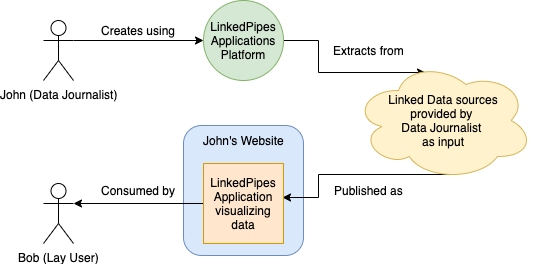
\includegraphics[width=10cm]{lpa_user_story.png}
    \caption{A sample user story describing usage of \lpa{} platform}
    \label{fig:lpa_user_story}
\end{figure}

It is important to note that the creation and publishing aspects of the \lpa{} are one of the requirements for \lpas{} that will be described in detail in \autoref{chap:num_3}. 

\subsection{Components overview}
\label{sssec:lpa_preliminaries_component_overview}

At the lower level, the \lpa{} is a bundle of various complex services and database solutions communicating actively communicating between each other. 

\begin{figure}[h]
    \centering
    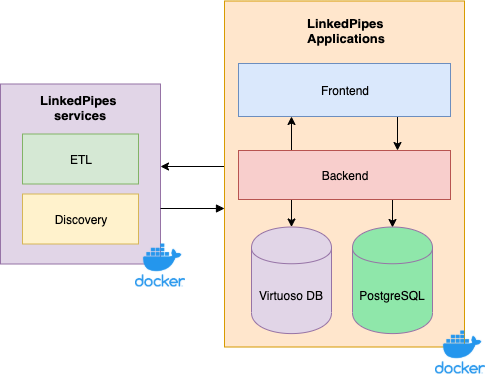
\includegraphics[width=12cm]{lpa_intro_architecture.png}
    \caption{High-level overview of \lpa{} platform}
    \label{fig:lpa_intro_architecture}
\end{figure}

Generally, we can categorize it into three main parts: 

\begin{itemize}
    \item \textbf{\fulllpa{}} - the main platform from LinkedPipes bundle that defines the functional and non-functional requirements for for \lpas{} project. Combines multiple database solutions for Linked Data, conventional SQL for storing user related records and implementation of a backend and frontend for creating applications.
    \item \textbf{\lps{}} - a set of external services provided from LinkedPipes bundle that \lpa{} heavily utilizes. Provides a toolset for identifying how linked data can be discovered, extracted, transformed and loaded into an RDF file for further processing.
\end{itemize}

\subsubsection{Frontend}
\label{ssssec:frontend_preliminaries}

As mentioned at the beginning of the chapter, the frontend provides a way for the user to interact with the \lpa{}. The Redux \footnote{\url{https://redux.js.org}} and React \footnote{\url{https://reactjs.org}} are the leading technologies to be used during implementation. The main terms related to \lpa{} frontend that are commonly reffered to in \autoref{chap:num_4} and \autoref{chap:num_5} are described as follows:

\begin{itemize}
    \item \textbf{React Component} - a JavaScript class or function that optionally accepts inputs, i.e., properties(props), and returns a React element that describes how a section of the UI (User Interface) should appear. 
    \item \textbf{Redux} - represents a container that stores various states of the web application per individual webpage.
    	\subitem \textbf{State} - refers to the single state value that is managed by the store and returned by getState(). It represents the entire state of a Redux application, which is often a deeply nested object.
        \subitem \textbf{Reducer} - specifies how the application's state changes in response to actions sent to the store.
        \subitem \textbf{Actions} - are payloads of information that send data from your application to your store. They are the only source of information for the store. You send them to the store using store.dispatch().
        \subitem \textbf{Selector} - is simply any function that accepts the Redux store state (or part of the state) as an argument, and returns data that is based on that state.
\end{itemize}

Additionally, the \lpa{} frontend is the main component that is going to be improved by \lpas{}. This is due to specifics of a \solid{} toolset where most of the open-source libraries are implemented in JavaScript programming language and are intended for usage in web based projects.

\subsubsection{Backend}

The function of the backend component is to provide a RESTful \acrfull{API} that is used by the frontend component to execute user-requested actions and can also be used by other developers to create their user applications. The backend then implements the communication protocols with external services from \lps{} bundle. 

\subsubsection{PostgreSQL} 

The \lpa{} platform is storing all information related to users of the platform in an instance of a PostgreSQL database \footnote{\url{https://www.postgresql.org}}. 

PostgreSQL, often Postgres, is an object-relational database management system (ORDBMS) with an emphasis on extensibility and standards compliance. It can handle workloads ranging from small single-machine applications to large Internet-facing applications with many concurrent users.

The entities stored in the database are described as follows:
\begin{itemize}
\item User accounts.
\item Running instances of LinkedPipes discovery processes. The LinkedPipes Discovery component is described in detail \autoref{ssssec:linkedpipes_services}.
\item Running LinkedPipes ETL pipelines. The LinkedPipes ETL component is described in detail in \autoref{ssssec:linkedpipes_services}.
\item Custom templates of data sources generated by users.
\end{itemize}

\subsubsection{Virtuoso DB}

Aside from PostgreSQL, another important database technology is OpenLink Virtuoso\footnote{\url{https://virtuoso.openlinksw.com}} which is used for storing all Linked Data sources processed by LinkedPipes ETL pipelines, and that is later used by \lpa{} visualizers. The important note to mention is that in contrast with PostgreSQL that is only used for all user-related information that needs to be stored, Virtuoso is only used for storing Linked Data. 

In general, Virtuoso is a middleware and database engine hybrid that combines the functionality of a traditional \acrfull{RDBMS}, \acrfull{ORDBMS}, virtual database, RDF, XML, free-text, web application server and file server functionality in a single system. Rather than having dedicated servers for each of the functionality mentioned above, Virtuoso serves as a universal server instance.

\subsection{\lps{}} 
\label{ssssec:linkedpipes_services}

The \lps{} bundle demonstrated on \autoref{fig:lpa_intro_architecture} consists of two open-source software solutions developed under the Faculty of Mathematics and Physics at Charles University in Prague. They serve as the providers of core Linked Data processing functionality for \lpa{} platform. Since a significant technical knowledge in Semantic Web is required to use the tools independently, the \lpa{} platform provides a layer on top of them to simplify interactions with those components and make it available for any generic \textit{lay} user. 

\subsubsection{ETL} 

LinkedPipes ETL is an RDF-based, lightweight \acrfull{ETL} tool for Linked Data \cite{etl}. It is not only a stand-alone application, but it also exposes an \acrshort{API} through which third-parties can execute the ETL process. In formal terms, a service performs the core computational work by querying the graphs of data sources provided by a user and attempting to transform that data into a format that can be later converted into an input for visualizations. 

\subsubsection{Discovery} 

LinkedPipes Discovery is a service used by \lpa{} platform to discover whether provided Linked Data sources can be processed and visualized by the platform \cite{discovery}. After a successful request sent to the Discovery service, it executes a session called \textit{Discovery session}. Upon successful completion of a Discovery session, the service generates specific files in JSON-LD format. Those files are called \textit{pipelines}. A pipeline describes how LinkedPipes ETL needs to extract the whole Linked Data set and store the data into a Virtuoso database, which is a component used by the LinkedPipes Applications platform described earlier. 
\chapter{Related work}
\label{chap:num_2}

This chapter provides an overview of currently available alternatives to \solid{} project, as well as research projects that share similarities with the core concepts of decentralized social platforms. The first set of sections provides a general description of alternative technologies, the last \autoref{sssec:comparison_of_technologies} provides a comparison between the alternative software solutions and \solid{}.

\section{Diaspora}

Out of all currently available solutions, the conceptually closest software platform to \solid{} is Diaspora \cite{diaspora_paper}\cite{diaspora_site}. In general, it is a decentralized social network platform that enables users to choose the server where their data is hosted and even run their own data hosting server. In that sense, it is similar to \solid{}. However, the main focus in Diaspora is to act as a social network, where social data is shared between users using specific APIs, and not running diverse applications on stored data. Unfortunately, it does not offer a well-defined way to use the same data with different applications. Note that Diaspora uses the term pod to refer to a data hosting server. A Diaspora POD is what \solid{} would refer to as a \solid{} server.

\section{WebBox}

WebBox is a decentralized social network platform that decouples data from applications \cite{webbox}. As \solid{}, it stores user’s data as Linked Data in a decentralized way. Also similar to \solid{}, system rely on WebID for decentralized identity, authentication, and access control. In WebBox, each data storage service exposes a SPARQL endpoint, and applications manipulate the data via SPARQL queries and updates, or via HTTP GET requests. In contrast, \solid{} offers the full power of LDP for simple data interactions (e.g., hierarchical data organization, fine-grained manipulation) and additionally allows the use of link-following SPARQL for complex data retrieval. It also works as a generic storage platform upon which a significantly larger number of applications can be built. As a last remark, WebBox was mainly mentioned due to the similarities in functionality with \solid{} project, however, the platform was never released out of the bounds of a research prototype.

\section{OwnCloud}

OwnCloud \footnote{\url{https://owncloud.org}} is a self-hosted open source file sync and share server. In regards to previously defined requirements, this solution is somewhat too generic to the goals of the project, but due to certain features such as decentralization of the storage using manually setup instances, and various scalability features, building a platform based on the provided API is possible. Similar to Dropbox, Google Drive, Box, and others, ownCloud lets you access your files, calendar, contacts, and other data. You can synchronize everything between your devices and share files with others. In contrast with \solid{}, the solution is still a generic cloud storage. It does not support Linked Data out of the box and does not provide a trivial way to decouple data from applications using the data. 

\section{Mastodon}

Mastodon is an online, self-hosted social media, and social networking service \cite{mastodon}. It allows anyone to host their own server node in the network, and its various separately operated user bases are federated across many different sites (called "instances"). These instances are connected as a federated social network, allowing users from different instances to interact with each other seamlessly. Mastodon is a part of the wider Fediverse, allowing its users to also interact with users on other platforms that support the same protocol, such as PeerTube, Misskey, Friendica and Pleroma.

Mastodon has microblogging features similar to Twitter, or Weibo, although it is distinct from them, and unlike a typical software as a service platform, it is not centrally hosted. Each user is a member of a specific, independently operated instance. Users post short messages called "toots" for others to see, and can adjust each of their post's privacy settings. The specific privacy options may vary between sites, but typically include direct messaging, followers only, public but not listed in the public feed, and public and posted to the public feed. The Mastodon mascot is a brown or grey woolly mammoth, sometimes depicted using a tablet or smartphone.

Because there is no central server for Mastodon, each instance has its own code of conduct, terms of service, and moderation policies. This differs from traditional social networks by allowing users to choose an instance which has policies they agree with, or to leave an instance that has policies they disagree with, without losing access to Mastodon's social network.

\section{Hubzilla}

Hubzilla \footnote{\url{https://fediverse.party/en/hubzilla/}} is a modular webserver based operating system which includes technologies for publishing, social media, file sharing, photo sharing, chat and more (including the ability to develop custom modules). These services are accessed and connected across server and administrative boundaries through the communication protocol Zot which provides a high level of privacy and security customization and a nomadic identity for the users. A webserver running Hubzilla is called a "hub".

\section{Centralized cloud storage solutions}

Modern commercial and enterprise cloud storage solutions provide a great set of features as platforms for any generic use cases when reliable file storage is needed. For instance, Google Cloud Storage \footnote{\url{https://cloud.google.com/storage/}} and Amazon AWS Storage \footnote{\url{https://aws.amazon.com/products/storage/}}. However, in contrast with \solid{}, this approach is the most distant from the main concepts of LinkedPipes Applications project’s requirements. As a main disadvantage of the approach is the fact that even though the developer is offered a great set of flexibility within the platform, the data storing aspects are not fully decentralized. It also means that the end-user is uploading his data into a centralized data silo where commercial terms of services policies regulate ownership of his data. Another issue is platform dependency meaning that migrating, sharing, and interchanging the data between platforms is not trivial since all interactions with data within storage are defined by a set of APIs and SDKs specific to the selected platform. 

\subsection{Pitfals of centralized cloud storages}

In the past, having control over content or information people store and access online was a common case for many technologies on the Web. However, during the past 20 years, that situation changed significantly. Various tech giants and media platforms like Facebook and Google gain control over the personal data of millions of users using their services. The data that is under the control of the fixed authority separated from the rest of the organization or community is often referred to as data silos.  From the standpoint of the company, having centralized control over the data of all users of their platforms brings many benefits. It simplifies the development of services within the organization, allows to perform various analytics processes and understand the users better. However, from the users perspective, it significantly reduces the control of their data stored within centralized platforms.

\section{Comparison of technologies}
\label{sssec:comparison_of_technologies}

A significant difference between Solid and services mentioned below is that \solid{} sets a standard way of operating through a data model (RDF) and does not dictate how instances should behave as part of a "federation". In addition to that, \solid{} is not just a software technology, and it represents specifications built on top of open web standards, an extensive set of guidelines for developers, a community of active researchers and contributors. When it comes to direct comparison, \solid{} could be defined as a lower-level abstraction than federated services like Diaspora and Mastodon in the sense that \solid{} can serve as an infrastructure for building those platforms. For instance, Diaspora and Mastodon could be integrated into Solid by allowing their users to sign in using their WebID, and then allow users to store the data produced by them on the services on their POD. 

\begin{table}[hbt]
\centering
\resizebox{\textwidth}{!}{%
\begin{tabular}{|c|c|c|c|c|c|c|}
\hline
\textbf{Technology} & \textbf{\begin{tabular}[c]{@{}c@{}}Provides Personal \\ Data Store?\end{tabular}} & \textbf{\begin{tabular}[c]{@{}c@{}}Is stored data\\ easily reusable?\end{tabular}} & \textbf{\begin{tabular}[c]{@{}c@{}}Has decentralized\\  infrastructure?\end{tabular}} & \textbf{\begin{tabular}[c]{@{}c@{}}Has Linked Data \\ support?\end{tabular}} & \textbf{\begin{tabular}[c]{@{}c@{}}Is Open \\ Source?\end{tabular}} & \textbf{\begin{tabular}[c]{@{}c@{}}Is used in \\ production?\end{tabular}} \\ \hline
\solid{} & Yes & Yes & Yes & Yes & Yes & No \\ \hline
Diaspora & Yes & No & Yes & Yes & Yes & Yes \\ \hline
WebBox & Yes & Yes & Yes & Yes & No & No \\ \hline
OwnCloud & No & No & No & No & Yes & Yes \\ \hline
Mastodon & No & Yes & Yes & No & Yes & Yes \\ \hline
HubZilla & Yes & Yes & Yes & No & Yes & Yes \\ \hline
\begin{tabular}[c]{@{}c@{}}Popular centralized cloud \\ storages\end{tabular} & No & No & No & No & No & Yes \\ \hline
\end{tabular}%
}
\label{tab:solid_comparisons_table}
\caption {A comparison table between \solid{} and alternative technologies with similar concepts.}
\end{table}

% TOD : hot to fix the table autoref ?

The table \TODO{use autoref} \ref{tab:solid_comparisons_table} provide a detailed comparison between \solid{} and technologies alternative to it. The columns indicate questions representing main features required from a technology to be able to use the benefits of Semantic Web, Linked Data, and RDF at full scale while preserving security and decentralized storing aspects. Both Diaspora and WebBox come very close to \solid{} in terms of provided functionality. However, as mentioned in their descriptions, Diaspora does not focus actively on storage and data decoupling aspects, and WebBox is a proof of concept project that is not available in production or has an open-source community. Similar to Diaspora, Mastodon and Hubzilla position themselves as platforms providing various social networking features to users. And finally, solutions like OwnCloud or popular centralized cloud storage solutions from Google, Microsoft, or Amazon provide convenient developer APIs for using their technologies. However, the technology itself does not preserve the ideas of decentralization and privacy-oriented data management. In contrast, as mentioned before, it provides an opposite functionality where data gets aggregated inside centralized silos under control of the organization providing the storage. 
To sum up, this section provided a brief comparison overview of alternatives to \solid{}. The following \autoref{chap:num_3} will give detailed reasoning for choosing \solid{} as a core technology for providing storage capabilities for \lpa{} and what makes it a better fit than its alternatives. 

\chapter{Analysis}
\label{chap:num_3}

The following chapter will start by providing a detailed set of functional and non-functional requirements from \lpa{} in regards to \lpas{}. Afterward, an analysis of the currently available development tools within the \solid{} ecosystem will be demonstrated. Additionally, as a continuation of comparison in \autoref{sssec:comparison_of_technologies}, a reasoning for choosing \solid{} as a core technology for implementing \lpa{} requirements will be explained.  The majority of the functionality of \lpa{} and \lpas{} were implemented by the author while working in parallel as a part of \lpa{} and as an individual contribution to the thesis. Therefore, to simplify the understanding of work on both projects and the difference between both contributions, the whole chapter is structured under the assumption that \lpa{} is a stakeholder with a working solution and \lpas{} is a technology yet to be implemented and integrated into \lpa{}. The consecutive chapter on architecture in \autoref{chap:num_4} and the implementation in \autoref{chap:num_5}, will guide the reader through established software development cycles where the result will be provided as a summary of implementation details in regards to requirements defined in this chapter.

Aside from definitions of specific requirements, it is important to note that there are three main \textit{actors} involved in statements of requirements. An actor is an individual entity interacting with the software components in requirements. Specific types are defined as follows:
\begin{itemize}
    \item \textit{Data journalists}, this category of actors are one of main target users of \lpa{} platform. They are defined as people familiar with, at least, basics of Semantic Web. They can provide Linked  Data sources to \lpa{} for further visualization and publishing of apps. They are also assumed to have an actual account in the \lpa{} platform.
    \item \textit{Lay users}, this is a second target category of users of \lpa{} platform. They do not have any prior experience with Semantic Web and in most cases, browse the published visualizers created by Data journalists. They are not obliged to have an actual account in the \lpa{} platform.
    \item \textit{\acrfull{LPA} Developers}, a developers implementing on \lpa{} platform codebase and main users of \lpas{} features, APIs and functionality to be developed. The majority of details in \autoref{chap:num_5} are focused on developing a developer-friendly software for this category of users.
\end{itemize}

\section{Functional requirements}
\label{ssec:functional_requirements}

In general, every functional requirement is defined as a description of services or features that software must offer. In this case \lpa{} defines a set of features expected to be handled properly by the \lpas{} project. The requirements are provided as a set of UML use-case \footnote{\url{https://www.uml-diagrams.org/use-case-diagrams.html}} diagrams as well as formal textual descriptions. 

\subsection{User authentication}

The user of the platform should be able to register an account in the application, log in, and log out. The requirement might seem unfitting to the purposes of \lpas{}. However, if \solid{} is considered to be used, it provides the fully functional authentication mechanisms based on WebID that can be used for generic platform authorization.

\begin{figure}[h]
\centering
\fcolorbox{black}{white}{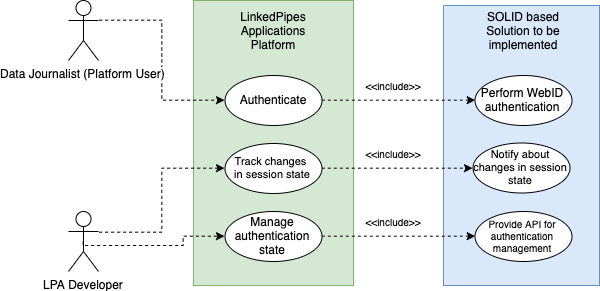
\includegraphics[width=0.7\linewidth]{lpa_authenticating_use_case.png}}
\caption{A UML use-case diagram describing user authentication requirement.}
\label{fig:lpa_authenticating_use_case}
\end{figure}

The UML diagram on \autoref{fig:lpa_authenticating_use_case} is described as follows:
\begin{itemize}
    \item \textit{Authenticate}, a platform must provide a way for Data Journalists (Platform Users) to authenticate via \lpa{} platform. This assumes that \lpa{} platform has an ability to communicate with the storage solution either integrated into \lpa{} codebase or presented as entirely separate service and \textit{perform WebID authentication}.
    \item \textit{Track changes in session state}, a platform must provide an API or a developer library for tracking any changes in the state of the authenticated platform user session. This assumes that the storage solution can inform the \lpa{} platform about such changes.
    \item \textit{Manage authentication state}, the platform must provide an API or a developer library for managing the authentication state of the users. This assumes that the core functionality is provided by the storage solution that exposes an API or a developer library toolset for developers to perform such interactions.
\end{itemize}

\subsection{Create, Store and Publish Application}

Creation, storing, and publishing of the application are the core features provided by the \lpa{} itself. However, the storage aspects are involved a lot when it comes to storing the created app. Consequently, publishing also consists of interacting with storage since an end-user expects the storage solution to have an identifier for his stored application.

\subsubsection{Creating and storing application}

User should be able to create an application within the \lpa{} platform and store it in his personal space in an authenticated storage. The storage solution can either implement a solution that stores entire application including the visualizer or generates a metadata configuration file that allows to re-create the entire application within \lpa{} platform from scratch.

\subsubsection{Publishing an application}

Another important requirement is an ability to publish the application and make it publically available for sharing the visualization to anyone via the permanent link. Furthermore, when a third party accesses this \textit{permalink}, the browser should open the \lpa{} website with the respective application opened, as configured by the publisher. The tool will also need to provide the ability to embed the published view into a data journalist's web page, for example, using an HTML \texttt{iframe} \footnote{\url{https://html.com/tags/iframe}}. 

\subsubsection{A diagram overview}

The \autoref{chap:num_5} describes the specific of creation, storing and publishing application requirements from perspectives of different actors involved. 

\begin{figure}[h]
\centering
\fcolorbox{black}{white}{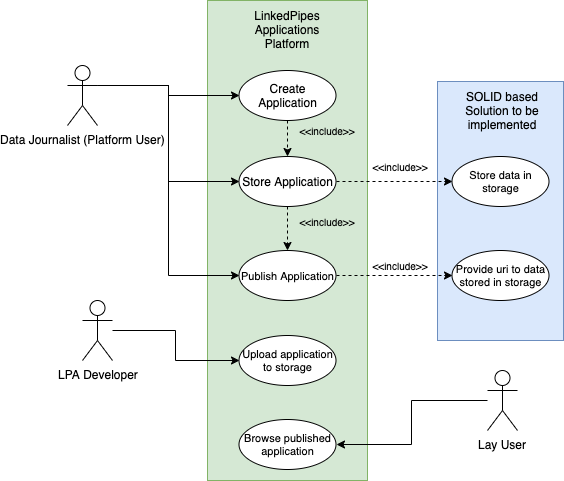
\includegraphics[width=0.6\linewidth]{lpa_creating_apps_use_case.png}}
\caption{A UML use-case diagram describing creation, storing and publishing application requirements.}
\label{fig:lpa_creating_apps_use_case}
\end{figure}

The diagram is described as follows:
\begin{itemize}
    \item \textit{Create application}, the platform provides an ability for Data Journalists to create an application. The process of creation of an application within \lpa{} also assumes that it is consequently \textit{Stored} and \textit{Published} via a set of interactions with storage. The publishing process is extended from storing an application because to publish an application, a configuration needs to be saved, and a URI for a stored resource in a \solid{} POD is extracted.
    \item \textit{Upload application to storage}, a platform provides an API or a library for LPA Developers to perform uploading of an application into the storage solution.
    \item \textit{Browse published application}, a platform provides a way for any Lay User to browse the published application created by Data Journalists. This is included as a part of the requirement since publishing is directly interacting with storage, and implementation of the requirement applies to both \lpas{} and \lpa{} platform.
\end{itemize}


\subsection{Managing storage and sharing published applications}

The last set of requirements is related to storage management and the sharing of published applications. The storage management requires a functionality that allows platform users to \textit{move}, \textit{copy} and \textit{create} data in their authenticated spaces in storage. The sharing requirement describes the functionality to allow users to share the applications they have published and control the access control settings to them. Since published applications require to be publically accessible to anyone, the platform needs to have a functionality to persist the configurations of the applications in a secure way. Moreover, the configurations for most of the published applications are represented as Linked Data. Therefore the persistent storage tooling needs to be optimized for files in RDF format.
 
\begin{figure}[h]
\centering
\fcolorbox{black}{white}{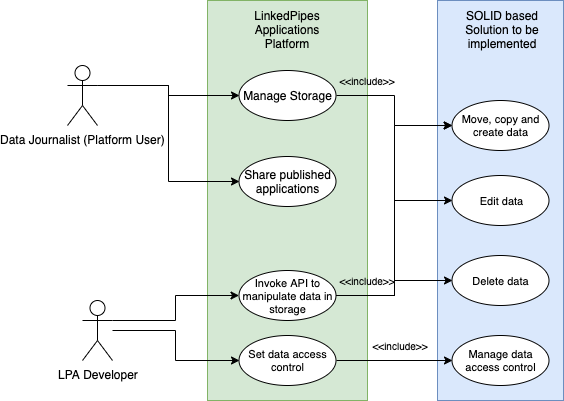
\includegraphics[width=0.6\linewidth]{lpa_managing_storage.png}}
\caption{A UML use-case diagram describing requirements on storage management and sharing of published application.}
\label{fig:lpa_managing_storage}
\end{figure}

As demonstrated on \autoref{fig:lpa_managing_storage}, the main elements are described as follows:
\begin{itemize}
    \item \textit{Manage storage}, the functionality of the platform to allow Data Journalists (Platform Users) to interact and manipulate data in their storage. In the case of \lpa{}, it is limited to visualizer application-related data only. 
    \item \textit{Share published applications}, an ability for Data Journalists to share the application with other users of the \lpa{} platform and set access control to the published applications.
    \item \textit{Invoke API to manipulate data in storage} assumes that \lpa{} provides tooling for their developers to interact with storage solution and invoke its APIs or libraries for manipulating data.
    \item \textit{Set data access control}, assumes that \lpa{} provides tooling for their developers to interact with storage solution and invoke its APIs or libraries for editing access control privileges to data.
\end{itemize}

\section{Non-functional requirements}
\label{ssec:non_functional_requirements}

In general, every non-functional requirement is described as the quality attributes of a software system, which contrasts with functional requirements that are specific to the exact behavior of the system. Within the scope of \lpa{} platform, the stated non-functional are rather an informal set of terms mainly related to \textit{reusability}, \textit{testability} quality attributes. 

\subsection{Compatibility with latest tools}

This general non-functional requirement states that an implemented software solution should be compatible with the latest tools of its technological ecosystem. For instance, if the designed software is a library using third-party packages, it needs to be generic enough to be compatible or have mechanisms to be resilient to any significant changes in third-party packages that it relies on.

\subsection{Clean APIs and libraries}

The solution needs to be implemented with code readability and reusability in mind. The primary users of the solution are developers of \lpa{} platform. Therefore it is essential to have an implementation based on a design that minds the established best practices and patterns of software engineering. 

\subsection{Continuous Integration and Delivery}

The implemented solution needs to maintain an optimized and fully automated Continuous Integration and Delivery pipelines. This ensures better possibilities in gaining contributors and planning future work and improvements on the solution as well as an infrastructure to debug and fix errors more effectively.

\subsection{Easy integration with \lpa{}}

The final solution needs to be able to integrate with the \lpa{} easily. Another important aspect is the solution to be integrated should not be entirely tied to the specified \lpa{} platform and should have the potential to be reused in other Linked Data based applications.

\subsection{Decentralized storage}

The Data Journalists, one of the primary target users of \lpa{} platform, should be able to choose any storage that is compliant with the technology stack of the solution. In other words, the platform should be able to support storing data in any personal space of such storage instances that are created, hosted, or owned by users directly or by the third-party providers.

\section{\solid{} development toolset}

Now, as the main requirements of the \lpa{} platform are defined, let us dive into the analysis of the \solid{} technology and tooling that it provides to understand better how it can be used to cover all stated requirements.

At the core \solid{} is a set of open specifications. At the current state of the project implementation, the community is most concerned about the persistence and representation of resources. However, such aspects as identity, authentication, and authorization are also vital parts of \solid{}.

A set of these standards are undergoing active implementation stage. Main contributors consisting of the core \solid{} development team, as well as the open-source community, develop the standards into various servers and tools. For instance, a \texttt{node-solid-server} library that implements a Solid server in Node and \texttt{rdflib.js} that allows you to manipulate RDF programmatically.

In addition to this, there is work done on supporting tools, such as Solid React SDK, that is created to allow developers to more easily get into developing apps with Solid. As part of this is the style guide that can be reused by others, not wanting to use the React parts.

\subsection{The \solid{} servers}

\solid{} itself represents a tech stack of complementary standards and data format vocabularies that are currently only available in centralized social media services. It also represents a Specification Document, serving as the main guideline for developers building their own apps and services. However, aside from that \solid{} also refers to a set of servers that implement its specification. 

\subsubsection{gold}

\texttt{gold} is a reference Linked Data Platform server for the \solid{} platform. The implementation is written in Go, based on initial work done by William Waites \cite{solid_gold_server}.

\subsubsection{node-solid-server}

Following solution is an implementation of a server based on \solid{} specifications in Node.js \cite{node_solid_server}.
One of the main advantages is that it could be launched as a \solid{} server on top of the local file-system. Interaction with server can be performed as follows:
\begin{itemize}
	\item Command line tool.
    \item Via \texttt{node-solid-server} library.
\end{itemize}

The provided server implementation was used as a main \solid{} server for the project due to compliance with main requirements for choosing the server. Those can be described as follows:
\begin{itemize}
	\item \textbf{Easy integration with current \lpa{} project}, specifically the frontend web project. This allows usage of provided `node-solid-server.js` library.
    \item \textbf{Active maintenance by open-source community}. Aside from that, this server implementation is considered to be a default option suggested by creators of \solid{}.
    \item \textbf{Support of \textit{WebID-TLS} and \textit{WebID-OIDC}}. This implies majority of WebID communications protocols,
    crucial to the user authentication and security aspects of the storage within \lpa{}. The WebID-TLS stands for a WebID authentication method over \acrfull{TLS}, providing an efficient and user friendly authentication on the Web \cite{webid_tls}. The WebID-OIDC is an authentication delegation protocol suitable for WebID-based decentralized systems such as \solid{} \cite{webid_oidc}.
\end{itemize}

\subsection{The \solid{} React development stack}

The main frontend library used in LinkedPipes Applications is React. In order to incorporate easier integration of aspects of \solid{} into the project, an analysis of React related \solid{} frameworks and libraries was performed. Even though, \solid{} community is yet to grow become stable and mature, it already provides a convenient set of libraries for React that were used as a main tools during implementation of the thesis project. 

\subsubsection{solid/react}

The main purpose of this library is to provide the following functionality:

\begin{itemize}
	\item Provide React developers with components to develop \solid{} apps.
    \item Enable React developers to build their own components for \solid{}.
\end{itemize}

\subsubsection{@inrupt/solid-react-components}

This libray is an official SDK provided by Inrupt for developing React Web applications for \solid{}. The package include various dependencies allowing:

\begin{itemize}
	\item Provide React developers with a set of easily customizable components interacting with \solid{} specifications.
    \item Provide a standardized visual design conventions based on Atomic Style.
    \item A set of cli commands for generating a template \solid{} projects.
\end{itemize}

\subsubsection{solid-auth-client}

The main purpose of this low level library is to provide ability to easily perform Authentication operations while interacting with \solid{} pods and servers.

At its core it is a browser library that allows your apps to securely log in to \solid{} data pods and read and write data from them.

\subsubsection{solid-file-client}

This library provides a simple interface for logging in and out of a Solid data store, maintaining a persistent session, and for managing files and folders. It may be used either directly in the browser or with node/require. The library is based on solid-auth-client and solid-cli, providing an error-handling interface and some convenience shortcuts on top of their methods and providing a common interface to the two modules.

\subsubsection{rdflib}

JavaScript RDF library for browsers and Node.js. One of the main contributors is Sir Tim Berners-Lee himself. The library is going to be used and described in detail in \autoref{chap:num_5}.

\subsubsection{@solid/query-ldflex}

The following library adds support of the LDflex language to \solid{} by:

\begin{itemize}
	\item Providing a JSON-LD context for \solid{}.
    \item Binding a query engine (Comunica).
    \item Exposing useful data paths.
    \item LDflex expressions occur for example on Solid React components, where they make it easy for developers to specify what data they want to show. They can also be used as an expression language in any other Solid project or framework.
\end{itemize}

\section{Why \solid{}?}
\label{sssec:why_solid}

Even though it is presented as a flawless dominating technology in \autoref{table:solid_comparisons_table}, it is, in fact, far from being perfect. Some of the disadvantages include:
\begin{itemize}
    \item \textit{Still under active research and development}, the project itself started back in 2016. Still, the real active traction and improvements had happened only within the past two years after community grew bigger, and the project gained popularity in the open-source community. It also means that there are still major changes in specifications introduces in every new iteration.
    \item \textit{Lack of actively maintained community libraries}, even though \solid{} organization on GitHub \footnote{\url{https://github.com}} actively updates and maintains its libraries for interacting with \solid{}. There is a large number of libraries developed by the community with tools that, in some cases, are more useful and popular. However, due to the \solid{} project still being actively developed, a lot of libraries outside of the scope of the organization become obsolete and outdated quickly.
    \item \textit{Still a lot of room for improving infrastructure for developers}. The project does not provide intuitive and user-friendly documentation. An average developer is required to have basic knowledge in Semantic Web, Linked Data, and working with RDF and SPARQL. However, the improvements were made in 2019, and eventually, the onboarding process into the technology will become easier for any developer.
\end{itemize}

Despite the disadvantaged mentioned above, the main reason for choosing \solid{} as a core for providing storage capabilities to \lpa{} was the fact that it is a very flexible and low-level technology.  Firstly,  as mentioned earlier, \solid{} represents multiple things at once. It is both a toolset with libraries for developers, a set of specifications, and an ambitious idea to a better World Wide Web where people own their data, and all information is linked together, preserving the semantic meaning. Of course, many attempts on decentralization were made before, but \solid{} differs from the others in the way that it does not target individuals in specific fields or domains of the Internet, it attempts to change the Internet itself, making it a better online space for everyone. And lastly, it demonstrated itself as a perfect fit for any application that requires any social aspects and involves dealing with any form of Linked Data, where \lpa{} platform and its requirements are compliant to all of the statements mentioned earlier.
\chapter{Architecture}
\label{chap:num_4}

The following chapter provides an overview of the architecture of \lpas. Explains the main components of the Storage as well as how it is being integrated into the LinkedPipes Applications platform.

\section{High-Level Overview}

While the majority of components were described in detail in \autoref{chap:num_1}, the overview architecture provided in this section shows more specific details on how all the external and internal components of the system are interacting. One of the essential details represented in the figure \ref{fig:lpas_high_level_architecture} is the separation between codebases of \lpa{} and \lpas{}. The \lpa{} Frontend imports the \lpas{} as an npm \footnote{https://www.npmjs.com} package and performs all interactions with \solid{} using the provided functionality of the package. In some sense, \lpas{} is being treated as an additional rudimentary backend and database layer on top of existing internal components inside \lpa{}. This is due to several functional requirements that \lpas{} package implements, such as \textit{user authentication}, \textit{operations to manipulate resources inside storage} and etc.

\begin{figure}[h]
\centering
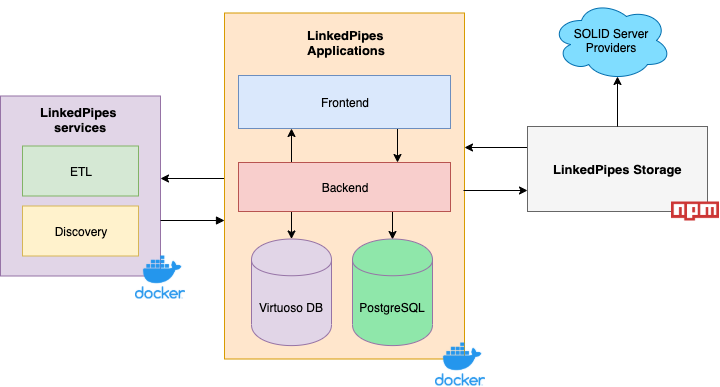
\includegraphics[width=14cm]{lpas_high_level_architecture.png}
\caption{High level overview of \lpa{} and \lpas{} interactions}
\label{fig:lpas_high_level_architecture}
\end{figure}

As additionally demonstrated, the figure \ref{fig:lpas_high_level_architecture} also has Docker icons displayed under some modules. The icons indicate where the production-ready service is hosted. For instance, in the case of the \lpas{}, the end goal is the npm registry, while \lps{} and \lpa{} are all hosted in the docker registry where each internal component is a docker container.
The generic interaction flow usually involves direct communication between the \lpa{} frontend and \lpas{} package. The internal frontend component has various React components implemented using the \lpas{} package that provides navigation and interaction with \solid{} Pods. While the package is designed under the assumption that the \lpa{} is the only user of the package, some abstractions are generic enough and have the potential to be used outside of the scope of the main functional requirements. The implementation chapter will also cover a generic use-case on how quick start \CONSIDER{how to start quickly} with application development based on \solid{}.

\subsubsection{The evolution of solid specifications}
At the moment of writing this chapter, the official \solid{} specification reached version \texttt{0.7.0} \footnote{\url{https://github.com/solid/solid-spec/blob/master/CHANGELOG.md}}. Introducing many changes and improvements, it also adds an extra layer of complexity with every release, changing some of the conventions, or updating some fundamental paradigms. As a result, when \lpa{} was initially implemented, it was based on an older specification and older versions of \texttt{node-solid-server}, that had a simpler and more extensive ability to manipulate ACL files. The work within this project, however, was focused around putting efforts into making it generic enough so that people could use it as a guideline for any started \solid{} apps, while the implementation will fit all \lpa{} requirements.

The main note to mention for the further section in this chapter is that the architecture design was derived from relying on the official specification of \solid{} while also referring to the provided functionality of \texttt{NSS} that does not always strictly follow the guidelines in the specification. 


\section{Storage}
\label{ssec:storage}

The initial architecture and implementation draft of \lpas{} were different from what is presented in this chapter.  \solid{} related logic was firstly a part of the \lpa{} codebase. Therefore, significantly complicating unit testing and making it hard to define the scopes of the \lpa{} and \lpas{} projects implementation. Later on, a decision was made to separate the logic of the \lpas{} and move it in the separate codebase. The majority of abstractions that were initially designed to be inside the \lpa{} codebase, consisted of various wrappers and crud functions to interact with \solid{} servers. Their design was refined and aggregated into specific abstractions, each responsible for covering the functional requirements from \lpa{} project.

\begin{figure}[h]
\centering
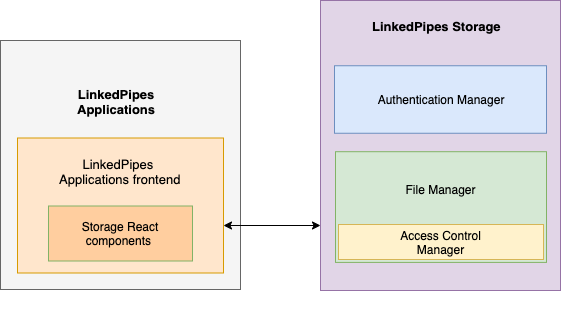
\includegraphics[width=14cm]{lpas_high_level_abstractions.png}
\caption{Main abstractions of \lpas.}
\label{fig:lpas_high_level_abstractions}
\end{figure}

Let us start by describing the main abstractions providing the functionality of \lpas{}.

\subsection{Authentication Manager}
\label{sssec:authentication_manager}

The Authentication Manager is responsible for wrapping \solid{} WebID based authentication logic into a simple and developer-friendly abstraction At the moment of writing this, the official \solid{} specification states to support the following protocols:
\begin{itemize}
\item WebID-TLS  - is one of the primary authentication protocols that rely on WebIDs instead of usernames. The passwords are replaced with certain cryptographic certificates as bearer tokens and are stored within the user's browser.
\item WebID-OIDC - alternative authentication protocol based on OAuth2 and OpenID Connect protocols and adjusted to support the concept of WebID. This is, in fact, the first authentication option provided by \lpas{}, later chapters will provide the reasoning behind why this ended up being a more intuitive option to cover the authentication requirement for \lpa{}.   
\end{itemize}

As already mentioned in chapter \ref{chap:num_3}, the usage of \textit{WebID} protocols is one of many benefits of \solid{}, in contrast with popular authentication protocols used in centralized silos, it is completely agnostic to specific authentication mechanisms, allowing our single abstraction to support any arbitrary \textit{WebID-OIDC} compliant \solid{} provider. 


\subsubsection{Interacting with frontend}

Sequence diagram on \autoref{fig:lps_authentication_sequence_diagram} demonstrate an example on how the Authentication Manager will be used within the \lpa{} Frontend and how it will interact with \solid{} Providers. The user agent entity represents a typical lay \lpa{} user interacting with the platform through the frontend component. The sequence flow consists of the following steps:

\begin{enumerate}
    \item The user clicks on the 'Authenticate' button. This is the starting point of this sequence diagram that serves as a trigger for \lpa{} to invoke the \lpa{} package.
    \item The frontend component calls the Authentication Manager and awaits for a callback. As the main input, it supplies the information about the \solid{} provider that the user would like to use.
    \item The Authentication Manager contacts the \solid{} provider and requests the provider authentication web page. Each provider conforming to \solid{} specification should contain that page.
    \item Depending on the browser environment of the user, he gets redirected to the provider's authentication web page either in a new browser tab or a popup dialog.
    \item The user selects the preferred authentication and inputs the credentials. At the moment of writing this thesis, popular \solid{} server implementations like node-solid-server support both WebID+TLS and WebID-OIDC specifications.
    \item The Authentication Manager receives the callback from the provider and sets the authenticated user session token.
    \item Frontend component receives the callback from the Authentication Manager, indicating that the user is authenticated.
    \item As the last step, the frontend redirects the user into the homepage dashboard of \lpa{} platform.
\end{enumerate}


\begin{figure}[ht]
\centering
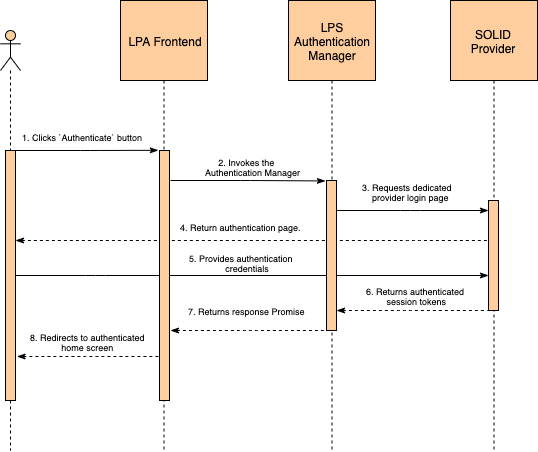
\includegraphics[width=12cm]{lps_authentication_sequence_diagram.png}
\caption{Sequence diagram for \textit{authenticate} operation invoked from \lpa{} frontend.}
\label{fig:lps_authentication_sequence_diagram}
\end{figure}


\subsection{File Manager}
\label{sssec:file_manager}

The File Manager is responsible for implementing the CRUD operations for the \solid{}  providers that are compliant with Linked Data Platform specification. The \gls{LDP} is a specification that is reused and extended in the \solid{} specification to describe the REST API for interacting with LDP Resources and LDP Containers \cite{lpd_specification}. LDP Resources and LDP Containers are, in some sense, the basic building blocks of any \solid{} POD, since they allow users to create any files and folders. 

As mentioned earlier, the \solid{} specification is re-using the LDP specification to provide a RESTful set of operations to interact with any compliant implementation of that specification. 

The LDP has an extensive set of resource types that are suited for defining the folder and files. However, the architecture provided is relying on two common resource terminologies that were simple enough to cover the requirements without complicating the design of the architecture. Those resources are defined as follows:

\begin{itemize}
%    Cite resource 
     \item Linked Data Platform Basic Container (LDP-BC), is a Linked Data Platform Basic Container. An LDP-RS representing a collection of linked documents that respond to client requests for creation, modification, and enumeration of its linked members and documents, and that conforms to the simple lifecycle patterns and conventions.
    \item An HTTP resource whose state is represented in any way that conforms to the simple lifecycle patterns and conventions, in other words any resource that can be \textit{created}, \textit{updated}, \textit{deleted} and \textit{red}. The LDP servers process the CRUD operations to manipulate the lifecycle of LDPRs.
\end{itemize}


\subsubsection{Creating resources}

The essential operation that is at the core of most functional requirements defined earlier is the ability to create a resource in a POD. Using the NSS server as a basis, the general convention for creating LDP resources is a POST HTTP request providing a link to the POD using the path where resource needs to be created. As demonstrated on \autoref{fig:lpas_create_resource} the creation consist of the following steps:
\begin{enumerate}
    \item \lpa{} frontend invokes the FileManager abstraction with a request specified in \texttt{ResourceConfig} abstraction. The configuration provided contains information on the type of resource, whether it is a folder or a file. Additionally, it describes the required information to identify the resource within the POD.
    \item \lpas{} constructs an HTTP POST request to create the resource in POD in \solid{} server, the response is forwarded asynchronously.
\end{enumerate}

\begin{figure}[h]
\centering
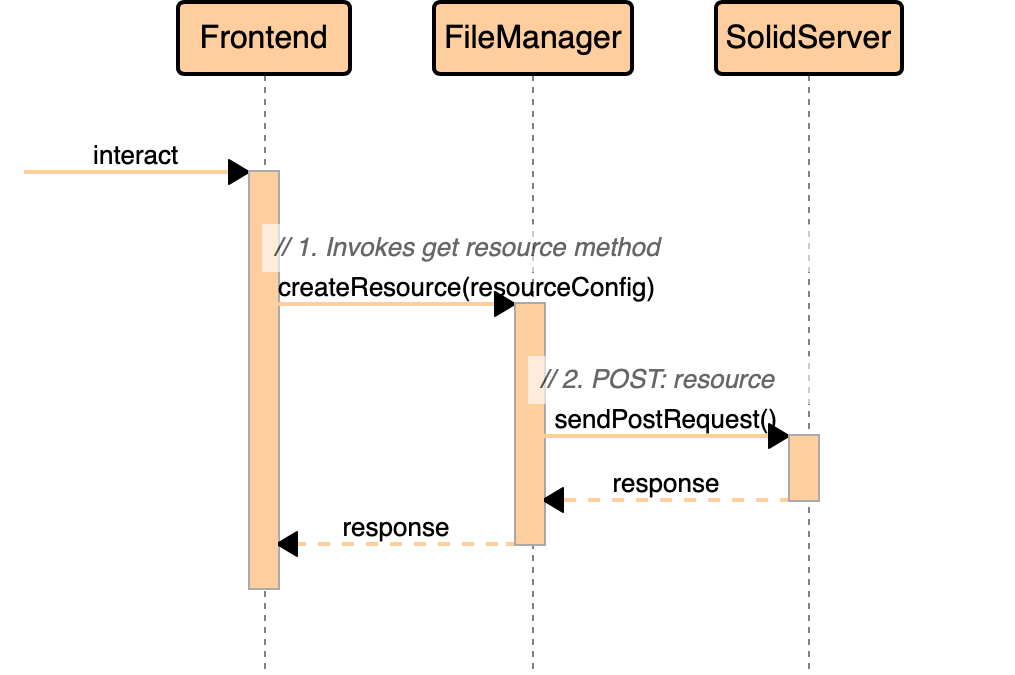
\includegraphics[width=8cm]{lpas_create_resource.png}
\caption{Sequence diagram for POST resource operation invoked from StorageFileManager.}
\label{fig:lpas_create_resource}
\end{figure}

\subsubsection{Reading resources}

Reading the resources demonstrated on figure \ref{fig:lps_get_resource_sequence} is a straightforward set of interactions with an \solid{} specification compliant server, and it can be described as follows:

\begin{enumerate}
    \item \lpa{} frontend invokes the FileManager abstraction with a request specified in \texttt{ResourceConfig} abstraction. The configuration provided contains information on the type of the resource, whether it is a folder or a file, as well as all required information to identify the resource within the POD.
    \item \lpas{} constructs an HTTP GET request to obtain the information from \solid{} server from the provider, the response is forwarded asynchronously.
\end{enumerate}


As demonstrated in the steps above, the LDP specification provides advantages by narrowing down the amount of resource lifecycle related calls as a set of elementary CRUD operations. Another important detail is that every single resource created by \lpas{} is an RDF file. We will cover more information and demonstrate why it is implemented in that way in the proceeding chapter.  
 
\begin{figure}[h]
\centering
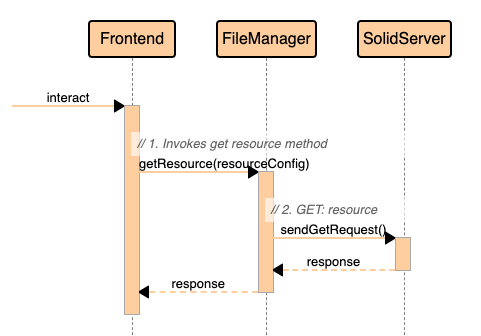
\includegraphics[width=8cm]{get_resource.png}
\caption{Sequence diagram for GET resource operation invoked from StorageFileManager.}
\label{fig:lps_get_resource_sequence}
\end{figure}

\subsubsection{Renaming resources}
\label{ssssec:renaming_resources}

The rename operation covers one of the functional requirements on the \lpa{} platform. It is based on a simpler CRUD operations such as \textit{create} and \textit{read} resource described in earlier sections. The goal of this function is to provide the ability for a \lpa{} developer to implement a functionality to let \lpa{} platform users to choose and manipulate their storage configuration folders.

The flow in the sequence diagram displayed in figure \ref{fig:lps_rename_resource} consists of the following steps:

\begin{enumerate}
    \item \lpa{} frontend invokes the FileManager abstraction with a request specified in the \texttt{ResourceConfig} abstraction, which is similar to the input steps in the previous sequence diagrams. 
    \item \lpas{} has a conditional check to see whether the new provided resource configuration is not accidentally the resource under the same title. This step is followed if the new path and title for a configuration are not equal to an old configuration.
        \begin{enumerate}
        \item Invoke the copy method that will depend on the resource either will copy it directly, if it is a file, or copy it recursively if it is a folder. For the sake of reducing the unnecessary details, the internals of the copy resource call is not displayed on this diagram.
        \item After copying the content of configuration into a new destination, the old resource is removed using the delete operation.
        \end{enumerate}
    \item \lpas{} returns a successful promise since no renaming is invoked in that case. 
\end{enumerate}

\begin{figure}[h]
\centering
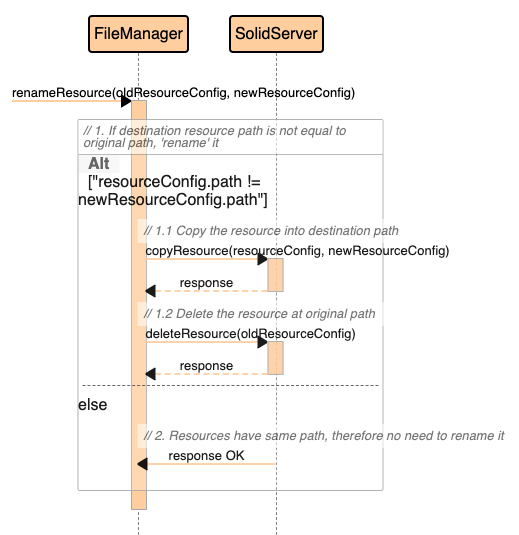
\includegraphics[width=10cm]{rename_resource.png}
\caption{Sequence diagram for a complex operation to rename a particular resource in StorageFileManager.}
\label{fig:lps_rename_resource}
\end{figure}

\subsubsection{Deleting resources}

The deletion of resources is slightly more complicated in comparison with the trivial GET, POST, PUT, and PATCH operations described in earlier sections. The main goal here is to differentiate the type of the resource, and depending on whether it is an LDP Basic Container or generic LDP Resource, act accordingly to delete all files under that resource. 
The flow from figure \ref{fig:lps_delete_resource} can be described as follows:

\begin{enumerate}
    \item Similar to the previous sequence flows, the action is triggered by an input request from \lpa{} frontend
    \item If the resource is and LDP Resource, FileManager trivially sends 
       a single DELETE request to the server and returns the response
    \item If the resource is an LDP Basic Container:
        \begin{enumerate}
        \item Invokes a method for recursively deleting the contents of a folder.
        \item Within that method, it performs a call that fetches the raw RDF describing the LDP Basic Container and parses the resources contained within using. 
        \item Iterate over files, remove them individually as in the first step.
        \item Iterate over folders, remove them individually as in the first step 
        \end{enumerate}
\end{enumerate}


\begin{figure}[h]
\centering
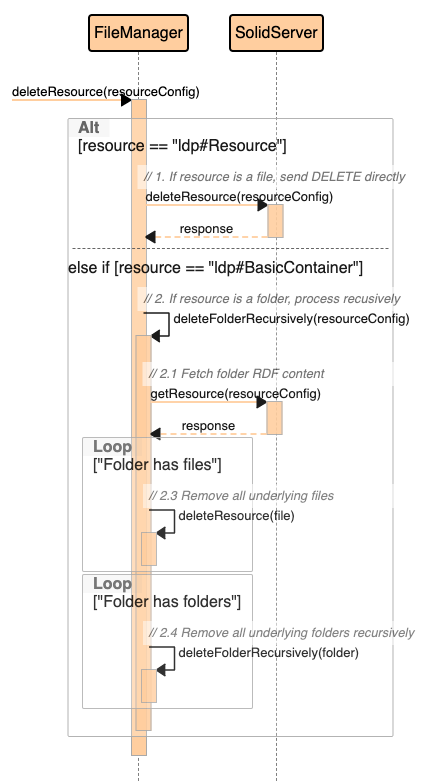
\includegraphics[width=8cm]{delete_resource.png}
\caption{Sequence diagram for a complex operation to delete a particular resource in StorageFileManager.}
\label{fig:lps_delete_resource}
\end{figure}


One of the assumptions made in this recursive operation is the interactions with ACL files when a recursive delete is performed. As mentioned in the introduction to this chapter, \solid{} community is still at its beginnings, and there are many significant improvements yet to introduce. In order to make the delete operation more generic, the DELETE interactions with ACL files had to be removed due to a more strict access policy established between providers of the server and \solid{} apps. The following section will dive deeper into Access Control Managements and related functionality.

\subsubsection{Classes overview}

File manager is the biggest of all three abstractions displayed on the figure \ref{fig:lpas_high_level_abstractions}. Therefore, in order to better describe the architecture of it, a more detail class diagram is provided on figure \ref{fig:lps_file_manager_class_uml}.

\begin{itemize}
	\item The core class available to \lpa{} developers is the \textit{StorageFileManager}. All of the functions inside are intended to be public, static and asynchronous. 
	\item \textit{ResourceConfiguration} is a wrapper for LDP Containers and LDP Resources. It allows a developer to specify \textit{title}, \textit{path} and \textit{type} of a resource. Most of the operations within the \textit{StorageFileManager} are operated with the resources encapsulated into \textit{ResourceConfiguration} classes. It also provides a few helper getters that allow to generate an absolute path to a resource within a pod. 
	\item The \textit{AccessControlConfig} is a subclass of \textit{ResourceConfig}. It allows to specify the access control modes to individual resources. Additionally, it introduces a few extra functions to generate the absolute path that includes the ACL file extension.   
	\item The \textit{SolidResource} is a simple interface that includes various details specific to the resource. Some of the fields provided are also directly used by \textit{StorageFileManager} abstraction during construction of CRUD calls to \solid{} providers.
\end{itemize}


\begin{figure}[h]
\centering
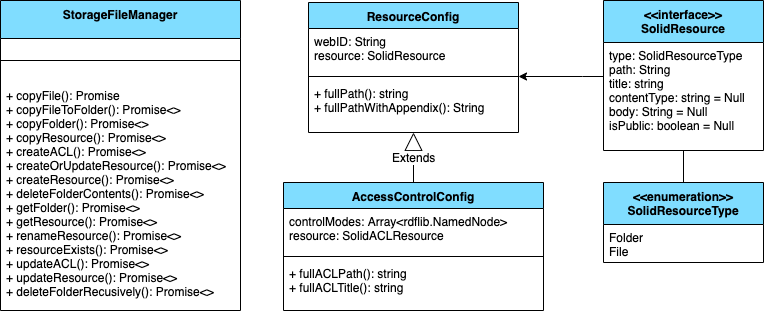
\includegraphics[width=14cm]{lpas_storage_file_manager_uml.png}
\caption{A higher level class diagram of classes contained within StorageFileManager abstraction.}
\label{fig:lps_file_manager_class_uml}
\end{figure}


\subsection{Access Control Manager}
\label{sssec:access_control_manager_arch}

The primary responsibility of the Access Control Manager is a subset under File Manager abstraction. It is designed to support the File Manager entities and provide an ability to wrap them with Web Access Control compliant settings. In other words, this allows a developer of \lpa{} to programmatically control the Read and Write access to any resource inside an arbitrary \solid{} POD by utilizing the developer-friendly interfaces and classes defined within the scope of this abstraction. Essentially, every ACL file is nothing more than yet another RDF resource with few extra features. Hence, the abstraction was placed under the File Manager since the core logic is concerned with similar resource lifecycle manipulations.

It is yet another wrapper on top of the functionality provided by any \solid{} compliant servers. In this case, being \solid{} compliant also assumes conforming to Web Access Control or WAC specification. It defines the so-called Access Control Resources, which are entities serving as the declaration of access control privileges for a specific resource. Within the context of \solid{} specification this means managing access rights to resources in \solid{} PODS for various WebIDs.

The main function provided by the abstraction is an ACL file generator. The flow on the figure \ref{fig:lps_acl_update_flow} demonstrated the process of generation, parsing, and serialization of ACL files: 

\begin{enumerate}
    \item Create Access Control triples for specified input resource configuration files.
    \item Create individual triples defining ACL configuration for a resource owner.
    \item Create individual triples for public access if the resource itself is marked as public.
    \item Gather and parse those triples into a rdflib abstraction representing an RDF Graph.
    \item Serialize this graph instance into a string representing a TTL file.
    \item Finally performs an HTTP call, that uses PUT to create an ACL file attached to a specified resource.
\end{enumerate}

This concludes the section demonstrating the essential abstractions within the \lpas{} package. The consecutive chapters dedicated to Documentation will cover and provide more details regarding less significant classes and utilities available inside the package.

\begin{figure}[h]
\centering
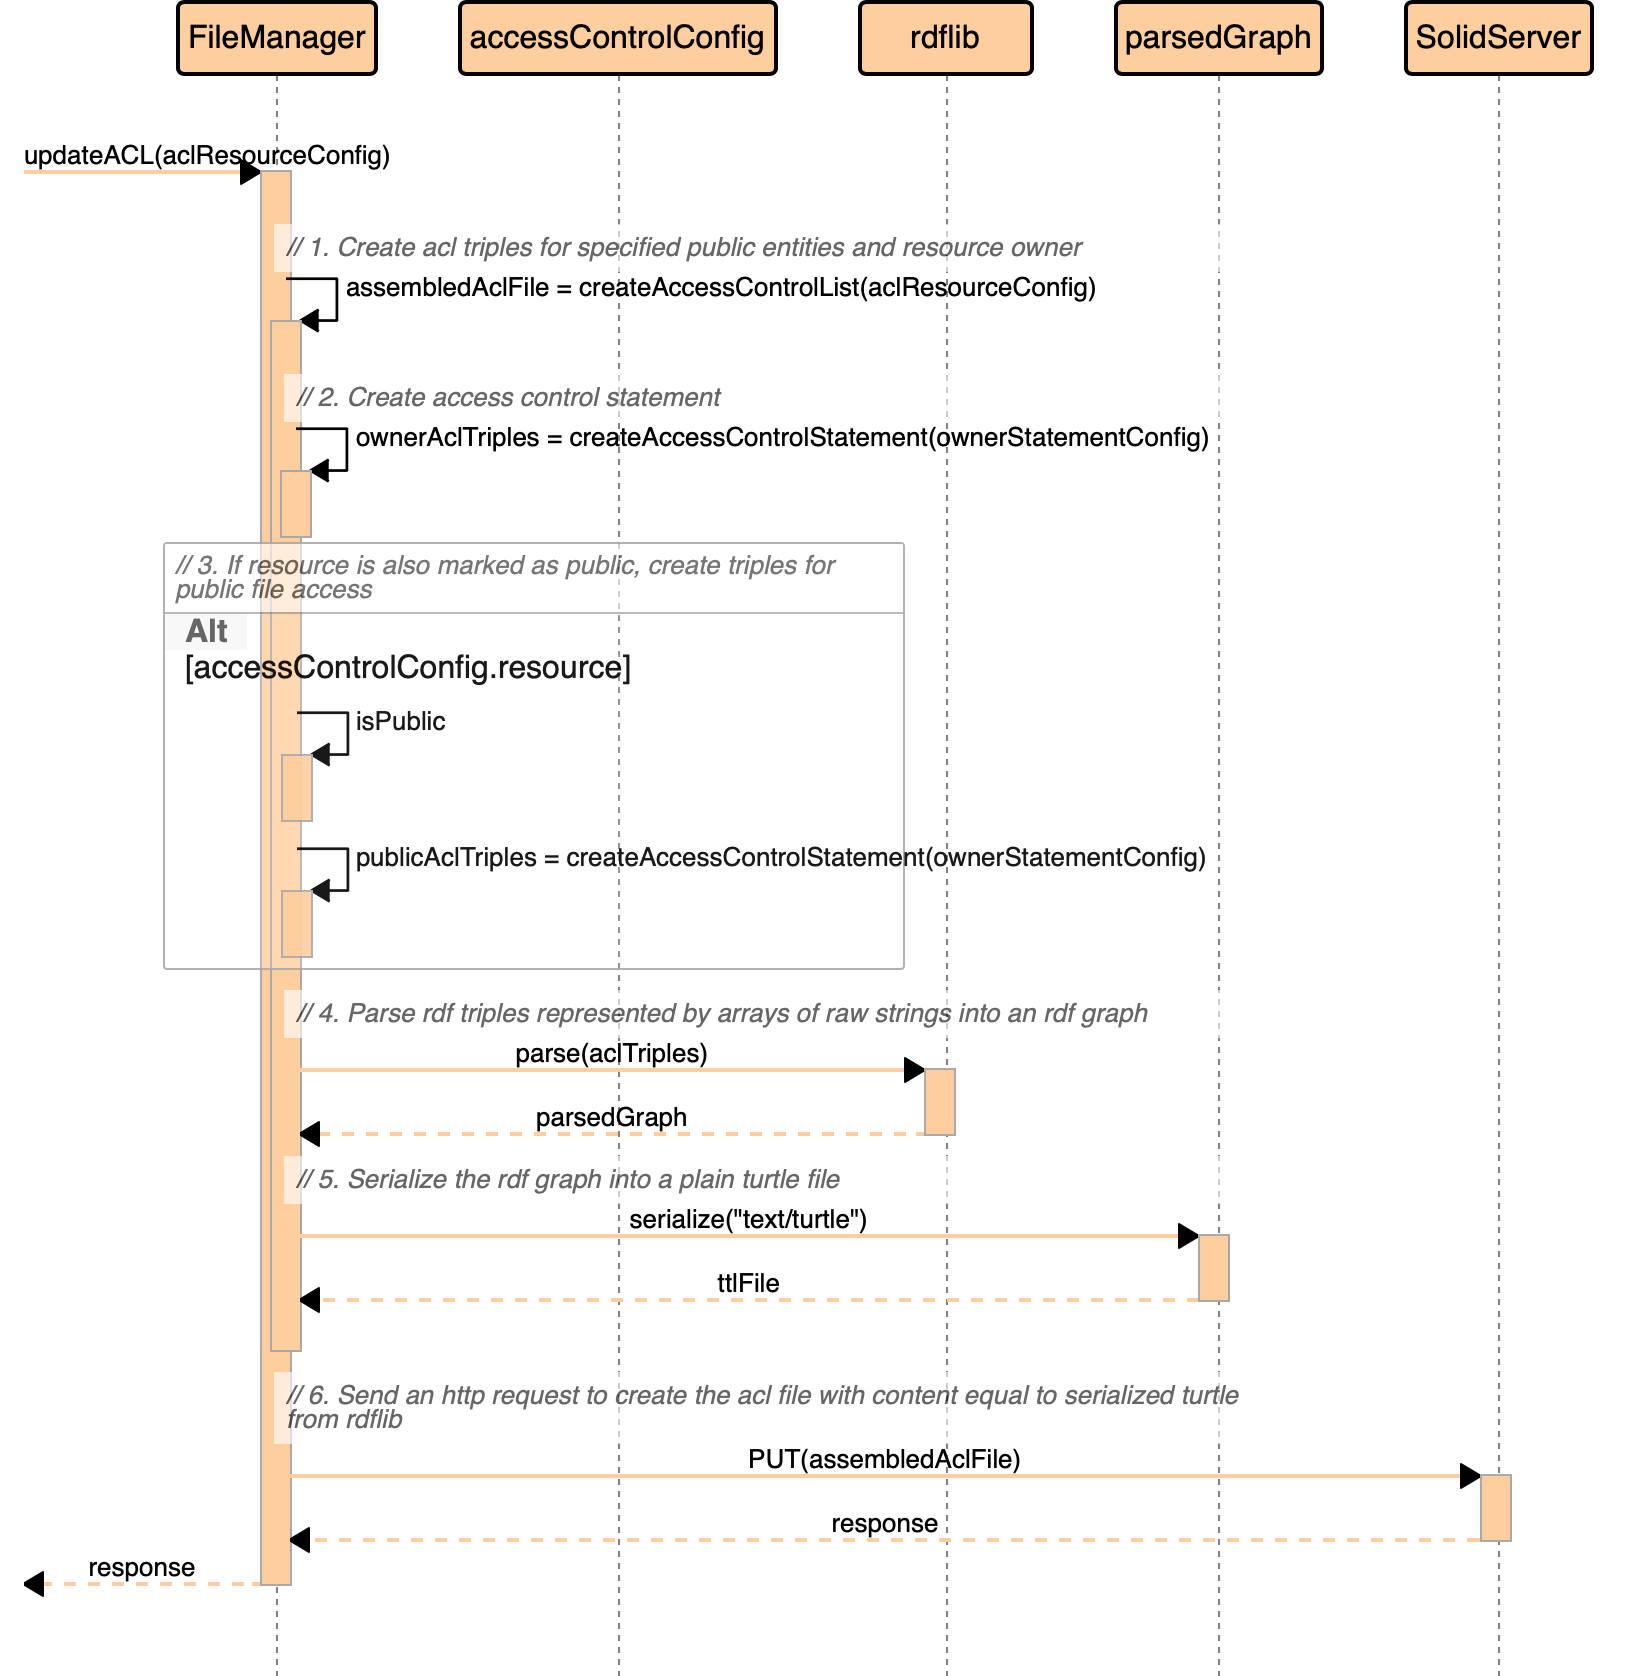
\includegraphics[width=14cm]{acl_update_flow.png}
\caption{A higher level class diagram of classes contained within StorageFileManager abstraction.}
\label{fig:lps_acl_update_flow}
\end{figure}


\section{LinkedPipes Applications Ontology}
\label{ssec:lpas_application_ontology_arch}

Relying on LDP specification extended by \solid{} was not the only goal while designing an architecture to satisfy the requirements of \lpa{}. It was also essential to use the advantages of Linked Data in general. As stated in introductory chapters, as well as the original paper \TODO{cite}, one of the significant benefits of any \solid{} compliant server is that everything is either an RDF file or has the metadata expressed as an RDF file \cite{solid_original_paper}\cite{solid_demo_paper}.  

The first task was to identify and analyze the kind of data \lpa{} is storing. The initial implementation on \lpa{} codebase was a simple application configuration JavaScript object that assembles all required configuration information for an application by the time a user of \lpa{} hits the \textit{Publish} button. In other words, we were given a JavaScript object to operate. Let us describe how this input requirement was taken into consideration while designing a solution that is both optimized for \solid{} and satisfies the requirement. 


\subsection{Using Web Ontology Language}
\label{sssec:using_web_ontology_language}

The Web Ontology Language or OWL, is a commonly used knowledge representation language used for:
\begin{itemize}
	\item Designing ontologies.
	\item Formalizing domains.
	\item Defining domain specific classes and properties.
\end{itemize}

As a first step, the JavaScript object that was used to represent \lpa{} configurations was formalized into a JSON Schema \footnote{\url{https://json-schema.org}}. Based on that Schema, the initial OWL ontology was designed using Stanford Protege \footnote{\url{https://protege.stanford.edu}}, which is a convenient open-source ontology editing tool. The class hierarchy on \autoref{fig:lpas_vocabulary_visualization} demonstrates the draft of the ontology created based on that Schema.

\begin{figure}[h]
\centering
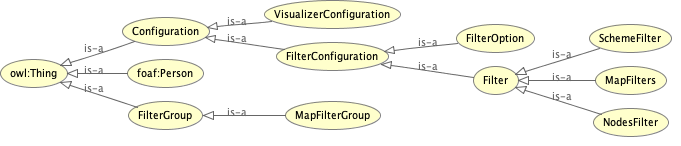
\includegraphics[width=14cm]{lpas_vocabulary_visualization.png}
\caption{A class hierarchy visualization of \lpa{} vocabulary.}
\label{fig:lpas_vocabulary_visualization}
\end{figure}

\subsubsection{foaf:Person}

The \textit{foaf:Person} node on \autoref{fig:lpas_vocabulary_visualization} refers to a WebID profile of an author of this configuration. Due to the generality of the WebID, there was no need to make a specific subclass from the foaf:Person class for that use-case.

\subsubsection{Configuration}
\label{ssssec:configuration}

The \textit{Configuration} class is the main generic abstraction for all \lpa{} configurations. Class hold the generic object properties that can be described as follows:
\begin{itemize}
	\item \textit{author}, this refers to the foaf:Person class stated before, and identifies the person with his WebID as an author of this \lpa{} configuration.
	\item \textit{published}, a date timestamp used to identify when configuration was created and published.
	\item \textit{title}, represents the title given to that \lpa{} visualizer.
\end{itemize}

The class is also a parent class for two subclasses titled \textit{VisualizerConfiguration} and \textit{FilterConfiguration}. More details on them provided in the implementation chapter. However, at this point, it is sufficient to understand that there are two main configuration types. One of them tied to the visualization, and the other is to filters that allow filtering information displayed on visualizers.

\subsubsection{FilterGroup}

The \textit{FilterGroup} class is closely related to Filter and FilterConfiguration and is used to reference the aggregation of visualizer specific filters. Since it does not necessarily need to inherit the object properties of FilterConfiguration, it is inheriting from generic \textit{owl:Thing} class.

\begin{figure}[h]
\centering
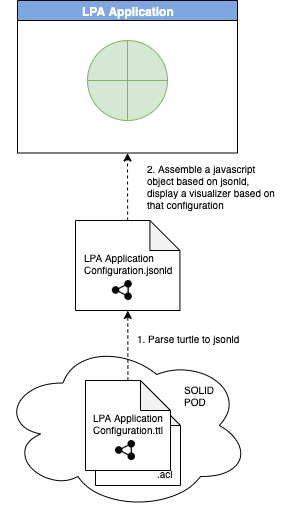
\includegraphics[width=6cm]{lpas_vocabulary_usage.png}
\caption{A formal representation of \lpa{} configurations expressed as RDF files using the \lpas{} vocabulary.}
\label{fig:lpas_vocabulary_usage}
\end{figure}

In order to simplify adoption of this ontology in \lpa{} frontend, the resulting ontology was converted into a JSON-LD Schema \footnote{\url{https://json-ld.org}}, as shown on \autoref{fig:lpas_vocabulary_usage}. However, due to some limitations in NSS, the individual \texttt{jsonld} configurations had to be converted into TTL files when stored in \solid{}. For more details on adoption and  implementation of this ontology refer to \autoref{chap:num_5}.


\section{Storage Component Design}
\label{ssec:lpas_storage_component_design}

It is important to note that the \lpas{} is not just the external package completely isolated from the \lpa{} frontend, it is also a set of React components that attempt to blend in into the user interface guidelines of the frontend. Now when the major components of the \lpas{} package as well as the \lpas{} vocabulary are described, let us dive deeper into the design considerations done on the frontend side inside the \lpa{} codebase. 

The \lpa{} frontend codebase was implemented using React\footnote{\url{https://reactjs.org}} and was utilising a modern stack of frontend development tools, all of those had to be taken into consideration to design React Component responsible for interactions with the storage. This section will cover the design conventions inherited from \lpa{} as well as a detailed overview of User Interfaces conforming to Material Design\footnote{\url{https://material.io/design}} conventions that were strongly utilized in \lpa{} frontend. In addition to that, it will also revisit the functional requirements and provide UI design proposals that are later implemented in the implementation section.

\subsection{Designing React Components}

At the root, \lpa{} frontend identifies two main types of components that are logically separated into folders titled as follows:
\begin{itemize}
	\item \texttt{Components} folder, these usually contain elements that are used in more than one webpage throughout the project, such as buttons, switches, image wrappers and etc.
	\item \texttt{Containers} folder, represent complex react components that are basically rendering individual webpages or sub-elements of webpages that deal with complex user interaction scenarios.
\end{itemize}

\subsubsection{Simple components}

Whenever an individual component needs to be implemented and it will be used in multiple webpages throughout the project, it is being placed into \texttt{Components} folder.

There are two main types of components that can be placed into \texttt{Components} folder and have different design conventions:
\begin{itemize}
	\item Simple stateless component responsible for plain rendering.
	\item A complex component that needs to aggregate multiple sub-components, manage external state, internal states and etc.
\end{itemize}


This is not a strict guideline defined by \lpa{} developers. However, if a component becomes too complex, as demonstrated on figure \ref{fig:lpas_component_design} the intent is to split component into separate component responsible for rendering and component that manages states of the stateless component. This allows easier navigation within frontend codebase as well as faster code debugging. 

\begin{figure}[h]
\centering
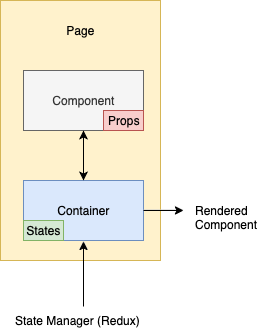
\includegraphics[width=7cm]{lpas_component_design.png}
\caption{React container abstraction decomposition following \lpas{} design conventions.}
\label{fig:lpas_component_design}
\end{figure}

Therefore, the logical decomposition of components by their complexity is the concludes the only major design convention that was required by \lpa{} frontend. Let us go over the details of each individual component in the following sections.

\subsection{Authentication View}
\label{sssec:architecture_auth_view}

Authentication is the entry for the \lpa{} platform, and \lpas{} covers the design and implementation of that view since \lpa{} relies on \solid{} to perform the WebID authentication. 

As previously demonstrated in \autoref{sssec:authentication_manager}, the \lpas{} package handles the authentication by redirecting the requests and responses between the browser of the user and the \solid{} provider server. The mock user interface on \autoref{fig:lpas_authenticate_mock} demonstrates a basic mock for a authentication webpage. There are several ways to authentication available to a \lpa{} user with a WebID profile in any \solid provider:
\begin{itemize}
    \item \textit{Provider authentication}, user clicks on a dropdown pane and selects the name of the default providers. The default providers supported by \lpas{} are \textit{inrupt.net} \footnote{\url{https://inrupt.net}} , \textit{solid.community} \footnote{\url{https://solid.community}} and a self-hosted LinkedPipes server available at \textit{lpapps.co:8443} \footnote{\url{https://lpapps.co:8443}}.
    \item \textit{WebID authentication}, similar to previous option but instead user is able to provide his WebID and be redirected right into the login page of his provider.
\end{itemize} 

\begin{figure}[h]
\centering
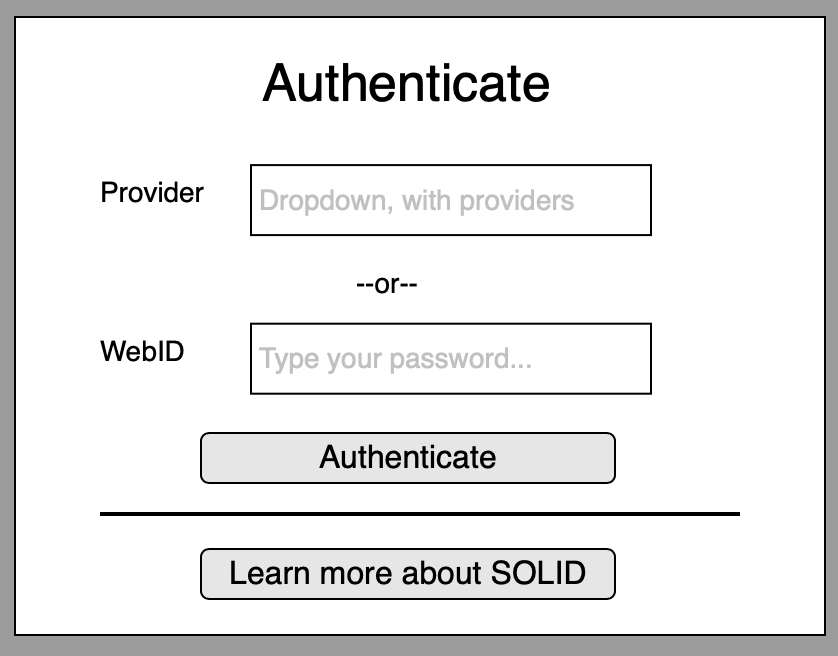
\includegraphics[width=7cm]{lpas_authenticate_mock.png}
\caption{Mock UI for Authentication webpage in \lpa{} Frontend.}
\label{fig:lpas_authenticate_mock}
\end{figure}

The additional user interface elements are defined as follows:

\begin{itemize}
    \item \textit{Authenticate} button executes the authentication sequence depending on the options that users have chosen, which are either Provider or direct WebID authentication.
    \item \textit{Lean more about \solid{}} redirects users not familiar with concepts of \solid{} directly into the home page of the inrupt project.
\end{itemize}
 

\subsection{Storage Dashboard}
\label{sssec:architecture_storage_dashboard}

Referring back to the functional requirements stated in the first chapters, the ability to interact with the \lpas{} is an essential feature allowing users of \lpa{} platform to manipulate their Applications. The mock displayed on \ref{fig:lpas_ui_dashboard_mock} is a webpage accessible via the home dashboard. There are two main display modes:

\begin{itemize}
    \item The \textit{My apps} tab, is a React component that fetches all RDF resources in root \lpas{} folder containing applications created by a user. 
    \item The \textit{Shared} tab is a React component fetching all RDF resources in a shared \lpas{} folder containing applications created and shared by a particular user with other users of \lpas{} platform.
\end{itemize}


\begin{figure}[h]
\centering
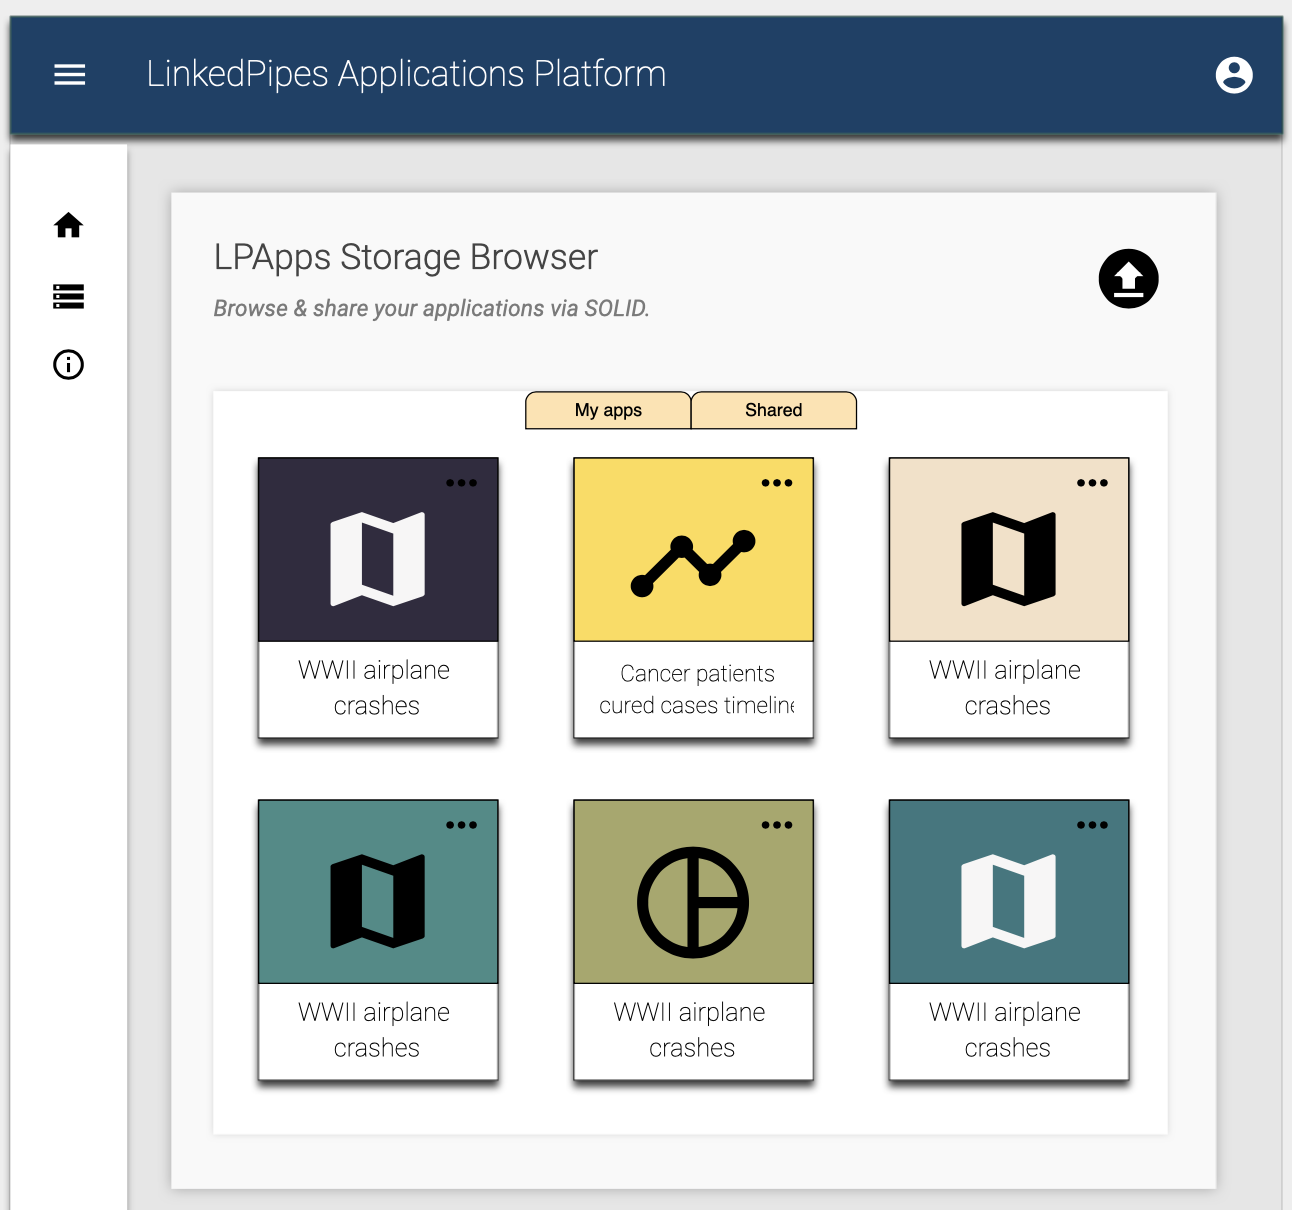
\includegraphics[width=7cm]{lpas_ui_dashboard_mock.png}
\caption{Mock UI for Storage Dashboard webpage in \lpa{} Frontend.}
\label{fig:lpas_ui_dashboard_mock}
\end{figure}



The idea behind the dashboard is that each card is a visual representation of \lpa{} configuration. As mentioned earlier in \autoref{sssec:using_web_ontology_language}, each configuration is expressed using the \lpas{} ontology and stored as an RDF file inside \solid{}. The card collection view pulls each of the configurations from the container, storing them in \solid{} and populates the content. 

The user of \lpa{} has a set of straightforward interactions that can be performed on card:
\begin{itemize}
    \item \textit{Clicking on card}, redirects the user to the webpage displaying the visualizer.
    \item \textit{Clicking on sub-menu icon}, reveals a popup where users can choose to delete, rename, or share the visualizer.
\end{itemize}


\subsection{Storage Control Panel}
\label{sssec:architecture_storage_control_panel}

An ability to authenticate, create, and publish an application using \solid{} are essential requirements stated by \lpa{}. However, users also need to have basic functionality to manipulate the data stored by the \lpas{} within their PODs. Therefore a mock design demonstrated on \autoref{fig:lpas_change_folder_mock} provides the basic functionality described as follows:

\begin{itemize}
    \item \texttt{Update} folder, allows users to switch their root folder into any other folder within their POD.
    \item \texttt{Copy} folder allows users to copy all content from the current root configurations folder into a new or existing folder.
    \item \texttt{Move} folder allows users to move all content from the current root configurations folder into a new or existing folder.
\end{itemize}


\begin{figure}[h]
\centering
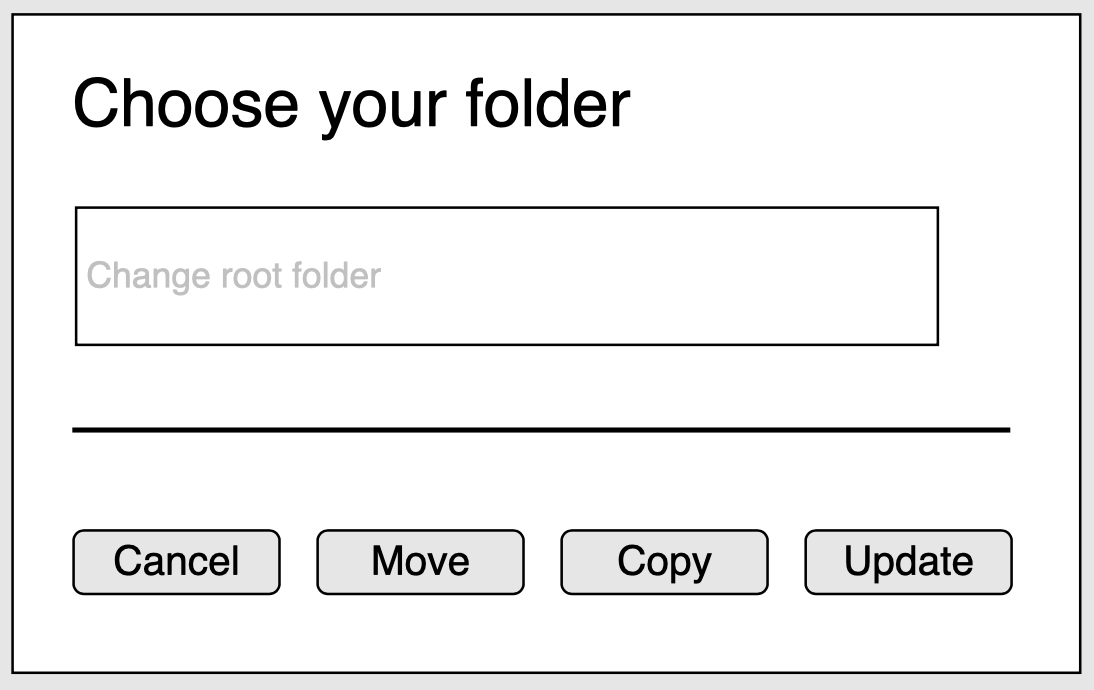
\includegraphics[width=6cm]{lpas_change_folder_mock.png}
\caption{Mock UI for Storage Dashboard webpage in \lpa{} Frontend.}
\label{fig:lpas_change_folder_mock}
\end{figure}

The diagrams in \autoref{ssec:storage} demonstrate the exact sequence of interactions between \lpa{}, \lpas{} and \solid{} providers when operations like \textit{move} or \textit{copy} folder are invoked.

To sum up, this chapter provided an overview of three major aspects of \lpas:
\begin{itemize}
    \item The npm package contains the core abstractions architectured to be separated from the \lpa{} with the intent to improve \solid{} related code maintainability and testing. The sequence diagrams of all main CRUD operations performed on RDF resources in \solid{} PODs.
    \item The \lpas{} ontology, an RDF vocabulary designed specifically for \lpa{} configurations, taking full advantage of \solid{}. In other words, giving an ability not simply to store the \lpa{} configurations, but also perform any complex querying on them using SPARQL.
    \item The frontend React components, the UI mocks of components inside \lpa{} frontend, conforming to conventions of the \lpa{}.
\end{itemize}
In the next chapter, a detailed review of the implementation of the architecture will be provided.



\chapter{Implementation}
\label{chap:num_5}

The following chapter is going to cover the implementation of \lpas{} package, the frontend components as well as the ontology. The first part of the chapter dedicated to the implementation of the package will provide a detailed overview of the decisions made on the development stack, the main challenges invoked in refactoring the original \lpa{} codebase, and making the \solid{} related functionality more generic. The frontend components section will dive deeper into the implementation of the mocks provided in \autoref{chap:num_4}, main decisions, and challenges while developing under React. The ontology \autoref{ssec:storage_ontology_implementation} will describe how the designed \lpas{} vocabulary was converted into a OWL file, converted into JSON-LD Schema and later integrated into the \lpa{} frontend. Lastly, an overview of the implementation results will be presented by reiterating over the defined \lpa{} requirements and how they were satisfied by the implementation.
 
\section{Storage Package}
\label{ssec_storage_package_implementation}

The initial implementation of \lpa{} frontend was written in \texttt{JavaScript ES6} \footnote{\url{http://es6-features.org}} and \texttt{React} framework. The development stack also included tools such as \texttt{Babel} \footnote{\url{https://babeljs.io}} compiler and \texttt{Webpack} \footnote{\url{https://webpack.js.org}} package bundler. 

\begin{figure}[h]
\centering
\fcolorbox{black}{white}{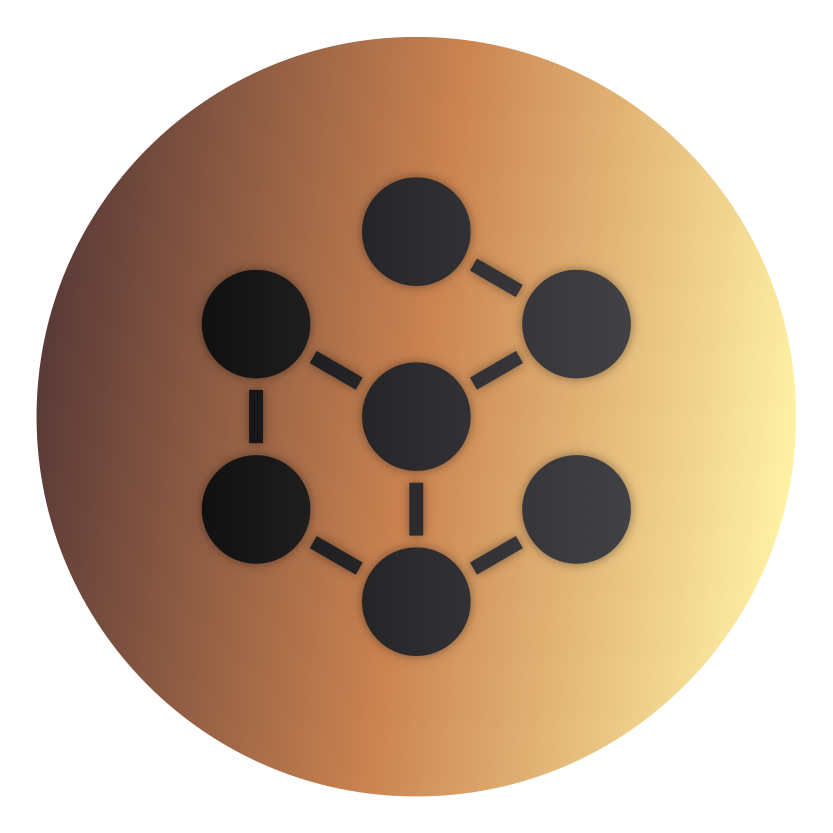
\includegraphics[width=0.4\linewidth]{lpas_package_logo.png}}
\caption{Official \lpas{} package logo designed by author.}
\label{fig:lpas_package_logo}
\end{figure}

As the number of features and functionality to cover was increasing, the decision was made to separate the \solid{} storage-related functionality into a separate npm package and call it \lpas{} package. This section will provide an overview of preliminaries chosen for the implementation of \lpas{} package as well as the specifics of implementations of each abstraction defined in \autoref{ssec:storage}. 

\subsection{Preliminaries}

As briefly mentioned earlier, there are several main libraries used inside the \lpas{} package:

\begin{itemize}
    \item \texttt{rdflib} is a low-level RDF library, that mainly provides the functionality to Read and Write RDF in many popular formats, a querying store and an ability to use SPARQL queries.
    \item \texttt{solid-auth-client}, a browser library that implements \solid{} specifications for providing authentication. This is the main library used to enable the authentication into \lpa{} platform.
\end{itemize}

Due to the complexity of the usage of the stated libraries, specifically \texttt{rdflib}, having an environment and a language that provides a fully-featured object-oriented programming and static type-checking would directly affect the code maintainability and usage. Hence, the codebase of \lpas{} was implemented using \texttt{TypeScript} \footnote{\url{https://www.typescriptlang.org}}. TypeScript is a strict syntactical superset of JavaScript that provides optional static typing and better object-oriented programming capabilities. When referred to files containing TypeScript code, the consecutive sections and chapters will refer to as \textit{TS} files.

\begin{figure}[h]
\centering
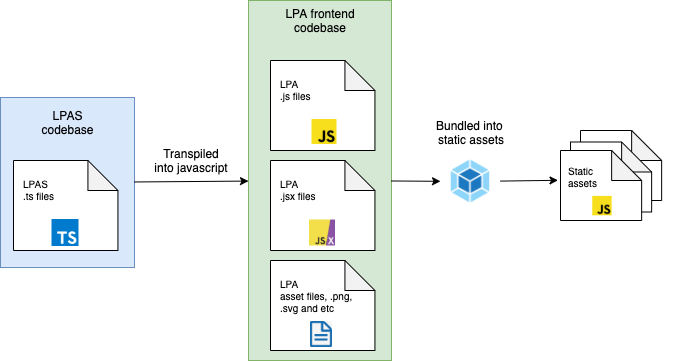
\includegraphics[width=12cm]{lpas_implementation_transpilation_diagram.png}
\caption{A diagram demonstrating the process of transpilation of \lpas{} package and bundling \lpa{} frontend with Webpack}
\label{fig:lpas_implementation_transpilation_diagram}
\end{figure}

As demonstrated on \autoref{fig:lpas_implementation_transpilation_diagram}, integrating the package into the \lpa{} codebase was done using the TypeScript compiler that allows transpilation into ES6 compatible JavaScript syntax. The package, as well as the rest of the \lpa{} codebase,  is later bundled into a set of static assets using Webpack. The assets mainly consist of a set of media files such as PNG and SVG files and a large JS file that contains the whole \lpa{} frontend. One of a few disadvantages with that approach is that the initial loading of the frontend might take a few seconds to load in the browser. Afterward, the interaction with the platform is seamless and does not involve any additional loading.

\subsubsection{Project structure}

The structure of the \lpas{} package is simple and straightforward and can be demonstrated as follows:

\begin{listing}[H]    
\begin{minted}[breaklines,frame=single,framerule=1pt,bgcolor=LightGray]{text}
- build       # Transpiled JavaScript code    
- markdown    # Markdown assets
- src         # Root project folder
  - lib       # Main library codebase
    - common  # Utilities and helper functions
       - ...     # TypeScript tests and core abstractions
  - types     # Custom user-defined type definitions
- docs        # Static html with library documentation
_ ...         # Readme and various configuration files
\end{minted}
\caption{\lpas{} package folder structure description.} 
\label{lst:lpas_folder_structure}
\end{listing}

The proceeding sections will describe the individual abstractions mentioned in \autoref{ssec:storage}.

\subsection{Authentication Manager}
\label{sssec:authentication_manager_implementation}

This section will continue the architectural description of the Authentication manager described in \autoref{sssec:authentication_manager}, describe the implementation and provide examples of how the abstraction is used inside \lpa{}.

The \textit{AuthenticationManager} is a Singleton class, instantiated only once and utilized both in the package itself as well as being invoked from \lpa{} frontend codebase. The reason for the class being implemented as a singleton is due to the fact that it wraps the functionality of \texttt{solid-auth-client} library, and it provides a singleton instance as well. Aside from providing the WebID authentication,  \texttt{solid-auth-client} implements a WebID OIDC specific \textit{fetch} functionality. The \textit{FETCH API} is originally a JavaScript API that provides an ability to send asynchronous HTTP calls. The implementation in \texttt{solid-auth-client}, is based on \texttt{isomorpic-fetch}, which is a third-party framework that implements the \textit{Fetch API} both for browsers and Node.js. Hence, the abstraction is used for:
\begin{itemize}
    \item Authentication, and ability to track the user session with callbacks. 
    \item Sending HTTP calls to \solid{} server.
\end{itemize}


\begin{figure}[h]
\centering
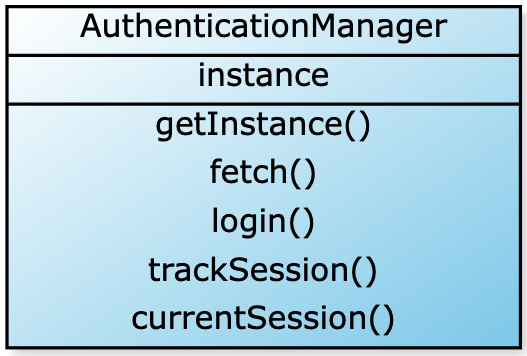
\includegraphics[width=6cm]{lpas_authentication_class.png}
\caption{A class diagram generated directly from a TypeScript file, demonstrating an implemented \textit{AuthenticationManager} abstraction}
\label{fig:lpas_authentication_class}
\end{figure}


In other words, once the client is logged in the \solid{} app, consecutive interactions are performed via \textit{fetch} function that is conveniently wrapped in the \textit{AuthenticationManager} abstraction.

As demonstrated on \autoref{fig:lpas_authentication_class}, the class consist of a set of public methods described as follows:
\begin{itemize}
    \item \textit{getInstance()}, this public method returns a singleton instance to an AuthenticationManager.
    \item \textit{fetch()}, a wrapper redirecting the call to \texttt{solid-auth-client} fetch method.
    \item \textit{login()}, a wrapper redirecting the call to \texttt{solid-auth-client} login method.
    \item \textit{trackSession()}, a method with asynchronous callback notifying the listener when a logout or login operation is performed.
    \item \textit{currentSession()}, a method returning the instance of a \texttt{solid-auth-client} Session object that contains relevant information about the authenticated user and his WebID. 
\end{itemize}

Referring back to \autoref{fig:lps_authentication_sequence_diagram}, there are several places in \lpa{} codebase where the \textit{AuthenticationManager} is invoked directly. The implementation of React components will be covered in the proceeding section, but the invocation of the abstraction itself can be described as follows:
\begin{itemize}
    \item \textit{Component layouts} are special high-level react containers that wrap every other container inside \lpa{} frontend. They are differentiated by \textit{public} and \textit{private}. The \textit{private} components reactively monitor the authenticated session of a user and redirect them back to the authentication screen whenever the value of the session becomes \texttt{undefined}. It is important to note that the session object from \textit{AuthenticationManger} is duplicated in \lpa{} frontend as a Redux state. Therefore, any changes in the original session object are reflected on that state and triggers re-rendering of layout components. 
    \item \textit{Authentication component functions}, are the functions being invoked when user attempts to perform the authentication. In other words, this is the input that triggers the flow demonstrated earlier on \autoref{fig:lps_authentication_sequence_diagram}.
    \item \textit{The App router}, the main class in \lpa{} that serves as an entry point and utilizing the \texttt{react-router} \footnote{\url{https://www.npmjs.com/package/react-router}} package, contains a function that invokes the \textit{trackSession()} method in \textit{AuthenticationManager}. This directly links to the session object and updates the changes from original session to internal Redux state.
\end{itemize}

The usage of both \textit{currentSession()} and \textit{login()} methods from \textit{AuthenticationManager} can be observed below:

\begin{listing}[H]    
\begin{minted}[breaklines,frame=single,framerule=1pt,bgcolor=LightGray]{javascript}
login = async (idp, callbackUri) => {
    const session = await AuthenticationManager.currentSession();
    if (!session)
      await AuthenticationManager.login(idp, {
        storage: localStorage
      });
    else {
      Log.info(`Logged in as ${session.webId}`);
      return session;
    }
};
\end{minted}
\caption{An implementation of \textit{login()} wrapper.} 
\label{lst:lpas_login_wrapper}
\end{listing}

To sum up, the \textit{AuthenticationManager} is a simple and straightforward singleton abstraction that wraps the \texttt{solid-auth-client} library and only necessary functions from the wrapped library to be used inside \lpas{} package. The examples of invocation from within the \lpas{} package are limited to directly calling the \textit{fetch()} method whenever an HTTP request is assembled and needs to be executed, more details on that will be described in a section dedicated to \textit{FileManager} abstraction.  

\subsection{File Manager}
\label{sssec:file_manager_implementation}

In this subsection, we will continue on the \textit{FileManager} abstraction described in \autoref{sssec:file_manager}, provide the specifics on implementation as well as a detailed overview of each method inside the abstraction.  

\begin{figure}[h]
\centering
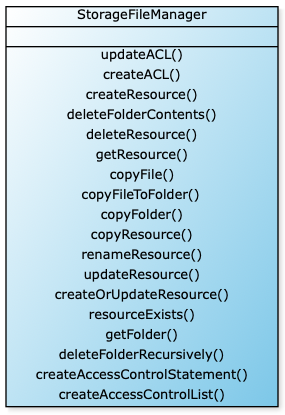
\includegraphics[width=5cm]{lpas_implementation_file_manager_diagram.png}
\caption{A class diagram generated directly from a TypeScript file, demonstrating an implemented \textit{FileManager} abstraction}
\label{fig:lpas_filemanager_implementation_class}
\end{figure}

Similar to the \textit{AuthenticationManager}, the \textit{FileManager} abstraction is implemented as a TypeScript class providing a set of public static methods. It is responsible for all core \textit{CRUD} operations with \solid{} resources. It is important to note that all HTTP requests to \solid{} server are made using the \textit{fetch()} method invoked via \textit{AuthenticationManager}. In other words \textit{FileManager} relies on \textit{AuthenticationManager} when performing HTTP requests. To follow up a class representation on \autoref{fig:lpas_filemanager_implementation_class}, the methods can be described as follows:
\begin{itemize}
    \item \textit{createResource()}, a function is responsible for creating new \solid{} resources. 
    \item \textit{deleteFolderContents()}, a function is mainly used for cleaning up the content of a particular folder. It iterates the contents and recursively deletes underlying folders and files.
    \item \textit{deleteResource()}, a function responsible for deleting individual resources from a \solid{} POD. Following the sequence flow presented on \autoref{fig:lps_rename_resource}, depending on the type of the resource it will either remove it directly or attempt to clean it recursively if the resource is an \textit{LDP-BC}.
    \item \textit{getResource()}, a basic function executing a GET call to obtain a resource content from a \solid{} server.
    \item \textit{copyFile()}, a basic function performing a copy operation on an \textit{LDPR}.
    \item \textit{copyResource()}, a generic method performing a copy operation on a resource. Depending on the type of the resource it either invokes the \textit{copyFile()} directly or, if resource is an \textit{LDP-BC}, it performs a recursive copying.
    \item \textit{renameResource()}, a method responsible for changing the title of the resource inside the \solid{} POD. In that case it simply means changing the absolute path to resource, where the name is the last element in the path. This function is described in detail on \autoref{ssssec:renaming_resources}. The operation involves invocation of several simpler methods from the \textit{FileManager} abstraction.
    \item \textit{updateResource()}, a generic function executing an HTTP PUT request for a particular resource.
    \item \textit{createOrUpdateResource()}, a method used in cases when a resource needs to be updated even if a different resource exists under that path. If a nothing exists under supplied path, resource will be created, if an object exists under particular path then it will be removed first.
    \item \textit{resourceExists()}, a method that executes the HTTP GET call to check if anything exits under specified path. The response is a simple boolean value.
    \item \textit{getFolder()}, a method that parses the contents of a particular folder and returns it as an array of underlying files and folders wrapped into a simple configuration abstraction. This is mainly used a part of any recursive operations involving folders.
    \item \textit{deleteFolderRecursively()}, a method used to execute recursive deletion of a particular folder. This is demonstrated in detail on \autoref{fig:lps_delete_resource} under a conditional block that is executed when resource is a folder.  
    \item \textit{createAccessControlStatement()}, \textit{createAccessControlList}, \textit{updateACL()}, \newline{} \textit{createACL()}, following methods can be found described in \autoref{sssec:access_control_manager_implementation}, as they relate to interacting with ACL resources.
\end{itemize}

It is important to note that the class is not a singleton in contrast with \textit{AuthenticationManager}. This is because all classes are exposed as public and static. The design makes the abstraction generic for many use cases within and outside the bounds of requirements of \lpa{}.

The \solid{} resource within the \lpas{} package is represented by \textit{ResourceConfiguration} abstraction that is a basic required input for most of the operations in \textit{FileManager} that involve execution of HTTP requests. The proceeding \autoref{ssssec:lpas_resource_config_implementation} will provide more details on implementation of this class and the relation to \textit{FileManager}.
 
\subsubsection{Resource Configuration}
\label{ssssec:lpas_resource_config_implementation}

One of the challenges when \lpa{} frontend initially contained the code for \solid{} interaction inside was the lack of any abstraction representing a particular \solid{} resource. There were several refactoring attempts to add basic ES6 classes, but maintaining the codebase was not trivial at all. Therefore, after introducing the \lpas{} package, the implementation of abstractions to represent the \solid{} resources was one of the first challenges. The \autoref{fig:lpas_resource_config_implementation} consist of two main entities:
\begin{enumerate}
    \item \textit{ResourceConfig}, a main class representing \textit{ResourceConfiguration} abstraction. 
    \item \textit{SolidResource}, an interface required for each object representing the \solid{} resource to be conforming to. 
\end{enumerate}

\begin{listing}[H]    
\begin{minted}[breaklines,frame=single,framerule=1pt,bgcolor=LightGray]{javascript}
enum SolidResourceType {
  Folder = '<http://www.w3.org/ns/ldp#BasicContainer>; rel="type"',
  File = '<http://www.w3.org/ns/ldp#Resource>; rel="type"'
}
\end{minted}
\caption{Definition of \textit{SolidResourceType} enumerator.} 
\label{lst:lpas_resource_type_enum}
\end{listing}

The \textit{SolidResource} interface consist of the following:
\begin{itemize}
    \item \textit{type}, an enumerator property represented on \autoref{lst:lpas_resource_type_enum}. Type is either a \textit{Folder} or a \textit{File}.
    \item \textit{path}, a \texttt{string} property representing a full absolute path excluding the filename itself. The reason why filename is excluded is to simplify the interactions within \textit{FileManager} class and provide more flexibility when operating with resources.
    \item \textit{title}, a \texttt{string} property representing the tile of the resource. The extension of the resource is not included.
    \item \textit{contentType}, an optional \texttt{string} property representing the content type header to be passed when constructing and HTTP request to  manipulate this resource. If value is not provided, a TTL extension is used by default.
    \item \textit{body}, an optional \texttt{string} property holding a content of the resource. The property is marked optional because there are cases when an empty folder resource need to be created, from an \lpa{} developer point, he does not need to provide any content to create an empty folder resource.
    \item \textit{isPublic}, an optional \textit{boolean} indicating whether the file is controlled only by the creator, owner or can have public read access. This is closely related to \textit{AccessControlManager} abstraction described in \autoref{sssec:access_control_manager_arch}. The proceeding section will describe the implementation of that abstraction in detail.  
\end{itemize}

The fact that \textit{SolidResource} is represented as the interface allows the objects conforming to eat to be constructed effortlessly and straightforwardly, similar to simply creating a \texttt{dictionary} object. The \textit{ResourceConfig}, on the other hand, wraps the object by providing additional information and functionality on top of the original resource object. The \textit{ResourceConfig} class consist of the following:
\begin{itemize}
    \item \textit{webID}, is a \texttt{string} property. The value should be assigned to the creator or owner of the resource. Within \lpa{} frontend, this value is usually holding the \textit{WebID} of the authenticated platform user.  
    \item \textit{resource}, is an \texttt{object} property conforming to \textit{SolidResource} interface. 
    \item \textit{fullPath}, a method returning a concatenated \texttt{string}, representing an absolute path to a resource.
    \item \textit{fullPathWithAppendix()}, a method returning a concatenated \texttt{string}, representing an absolute path to a resource with a \texttt{'/'} symbol. This is required in cases when an operation needs to be performed on a resource a developer wants to be sure that the absolute path will be constructed correctly for the underlying type. The \textit{folder} resource requires the symbol to be appended when dealing with the construction of ACL files. This will be described in more detail in the proceeding section dedicated to \textit{AccessControlManager} abstraction.
\end{itemize}

\begin{figure}[h]
\centering
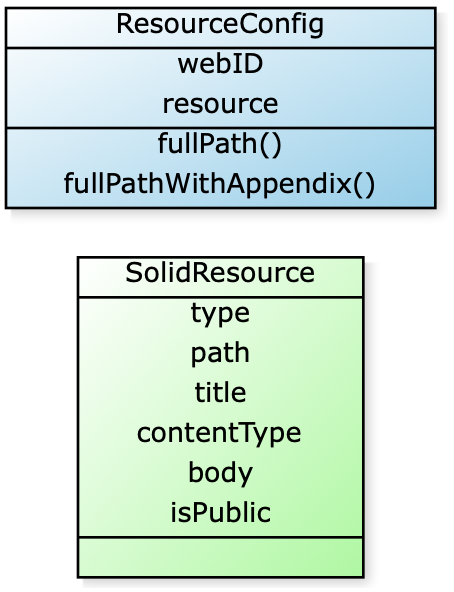
\includegraphics[width=5cm]{lpas_resource_config_implementation.png}
\caption{A class diagram generated directly from a TypeScript file, demonstrating implemented \textit{ResourceConfig} class and \textit{SolidResource} interface}
\label{fig:lpas_resource_config_implementation}
\end{figure}


The \textit{FileManager} class is extensively used throughout the whole \lpa{} frontend codebase. The examples below demonstrated various examples of invocations of the \textit{FileManager} abstraction from within the \lpa{} frontend codebase. It is important to note that the provided examples are generic enough to be applied to the development of any \solid{} application supporting the current iteration of \texttt{node-solid-server}.

\subsubsection{An example on creating a resource}

The example below demonstrated a simple use case on how \lpas{} package can be used to create a \solid{} resource using the \textit{FileManager} abstraction. 

\begin{listing}[H]    
\begin{minted}[breaklines,frame=single,framerule=1pt,bgcolor=LightGray]{javascript}
const folderConfig: ResourceConfig = new ResourceConfig(
        {
          path: rootResourceConfig.fullPath(),
          title: 'configurations',
          type: SolidResourceType.Folder
        },
        webId
      );
      
const response = await StorageFileManager.createResource(folderConfig)
\end{minted}
\caption{An example usage of \textit{FileManager} abstraction to create a folder in \solid{} pod.} 
\label{lst:resource_generation_example}
\end{listing}

In this particular case, a folder resource \textit{ResourceConfig} class instance is being created named \textit{configurationsFolderConfig}. Afterwards it is being passed to a public static \textit{createResource()} method that creates the resource as described on \autoref{fig:lpas_create_resource}. This concludes the description of the implementation of \textit{FileManager} abstraction. The proceeding section is dedicated to an \textit{AccessControlManager} abstraction, following up the first introduction in the \autoref{sssec:access_control_manager_arch}.


\subsection{Access Control Manager}
\label{sssec:access_control_manager_implementation}

This subsection provides details on implementation of the \textit{AccessControlManager} abstraction from \autoref{sssec:access_control_manager_arch} section. Despite being called a separate abstraction, it is in fact implemented as a set of additional public static methods inside the \textit{FileManager} abstraction as seen on \autoref{fig:lpas_filemanager_implementation_class} diagram. Essentially every ACL resource is yet another resource represented as \textit{LDPR} in \solid{}. However the functional implication of those resource are more specific and require extra information and functionality to operate with them. That is why it is separated conceptually as a different abstraction but is implemented inside the same class called \textit{FileManager}. 

Referring back to \autoref{fig:lpas_filemanager_implementation_class}, the main methods related to the abstraction are described as follows:
\begin{itemize}
    \item \textit{updateACL()}, a method constructing the array of RDF triples that is later serialized into a TTL and send as a body in HTTP PUT request to \solid{} server, replacing the previous resource under that path.
    \item \textit{createACL()}, a method constructing the array of RDF triples that is later serialized into a TTL and send as a body in HTTP PUT request to \solid{} server.
    \item \textit{createAccessControlStatement()}, a method constructing the array of RDF triples expressing access control for a particular WebID. 
    \item \textit{createAccessControlList()}, a method assembling an array of access control statements for multiple requested WebIDs using \textit{createAccessControlStatement()}, and as result serializes the array of statements into a raw TTL \texttt{string} using \texttt{rdflib}.
\end{itemize}

The functionality implemented by \textit{AccessControlManager} is not conforming to entire Web Access Control specification, since it was not needed and not required to satisfy the \lpa{} requirements. Therefore, methods described earlier such as \textit{updateACL()} and \textit{createACL()} as seen on \autoref{fig:lps_acl_update_flow}, were based on the default ACL files that \texttt{NSS} generates. At the moment of writing this thesis, the default ACL files generated by \texttt{NSS v5.2.0} looks as follows:

\begin{listing}[H]    
\begin{minted}[breaklines,frame=single,framerule=1pt,bgcolor=LightGray]{turtle}
@prefix : <#>.
@prefix n0: <http://xmlns.com/foaf/0.1/>.
@prefix n1: <http://www.w3.org/ns/auth/acl#>.
@prefix test: <./>.
@prefix c: </profile/card#>.
 
:owner
    n1:accessTo test:;
    n1:agent c:me;
    n1:default test:;
    n1:mode n1:Control, n1:Read, n1:Write.
:public
n1:accessTo test:; n1:agentClass n0:Agent; n1:default test:; n1:mode n1:Read.
\end{minted}
\caption{An example ACL resource in TTL describing access control for a folder} 
\label{lst:acl_file_example}
\end{listing}

As seen on \autoref{lst:acl_file_example}, the example describes access control privileges to a folder named \textit{test}. The first semantic triple contains a subject named \texttt{:owner}, and this refers to the WebID of the owner of this \solid{} POD. The predicates of the Owner subject can be described as follows:
\begin{itemize}
    \item \textit{accessTo}, the information resource to which the access is being granted. In this case, we are granting access to a folder named \textit{test}
    \item \textit{agent}, a person or an entity to whom the rights are being given. Since this is an owner of the \solid{} pod, the reference is given to himself.
    \item \textit{default}, this is a special predicate that behaves as follows. If the underlying resources have no ACL files specified, they will keep referring to parent resources until it will reach the resource containing the ACL file with \textit{default} predicate. In this case, the statement says that the underlying resources without explicitly set ACL files will have the same access control rights as the \textit{test} folder.
    \item \textit{mode}, a predicate describing the access control modes. In this case, the object is defined as follows: 
        \subitem \textit{Control}, a semantic object describing full read and write access to an ACL of the resource.
        \subitem \textit{Read}, a semantic object, is giving full read access to a resource.
        \subitem \textit{Write}, a semantic object is giving full write access to a resource.
\end{itemize}

On the other hand, the subject named \textit{public} only has an ability to \textit{Read} the folder and its content. The \textit{public} subject is just a generic simplification for cases when there is no need to set specific WebIDs explicitly. However, using ACL easily allows listing particular users as well, giving a lot of flexibility to have a very sophisticated access control privileges setup per any resource in a \solid{} POD. As mentioned earlier, the ability to manipulate access control to any resource and own your data is one of the core benefits proposed by \solid{} project. 

\subsubsection{Access Control Configuration}

Aside from the main \textit{AccessControlManager} abstraction, as demonstrated on \autoref{chap:num_1}, the original \textit{ResourceConfig} class from \textit{FileManager} required to be extended by introducing several subclasses called:
\begin{itemize}
    \item \textit{AccessControlConfig}, a subclass of \textit{ResourceConfig} that adds a property listing available control modes to a resource for specified WebID, and adds methods to construct the proper absolute path to a resource. The only difference between those methods and methods described in \autoref{ssssec:lpas_resource_config_implementation} such as \textit{fullPath()} and \textit{fullPathWithAppending()}, is that the hardcoded keyword ACL for files and hardcoded keyword \texttt{/.acl} for folder are being appended.
    \item \textit{AccessControlStatementConfig}, a subclass of \textit{AccessControlConfig}, contains additional references to \texttt{rdflib} nodes to simplify construction of ACL triples in \textit{AccessControlManager} abstraction.
\end{itemize}

\begin{figure}[h]
\centering
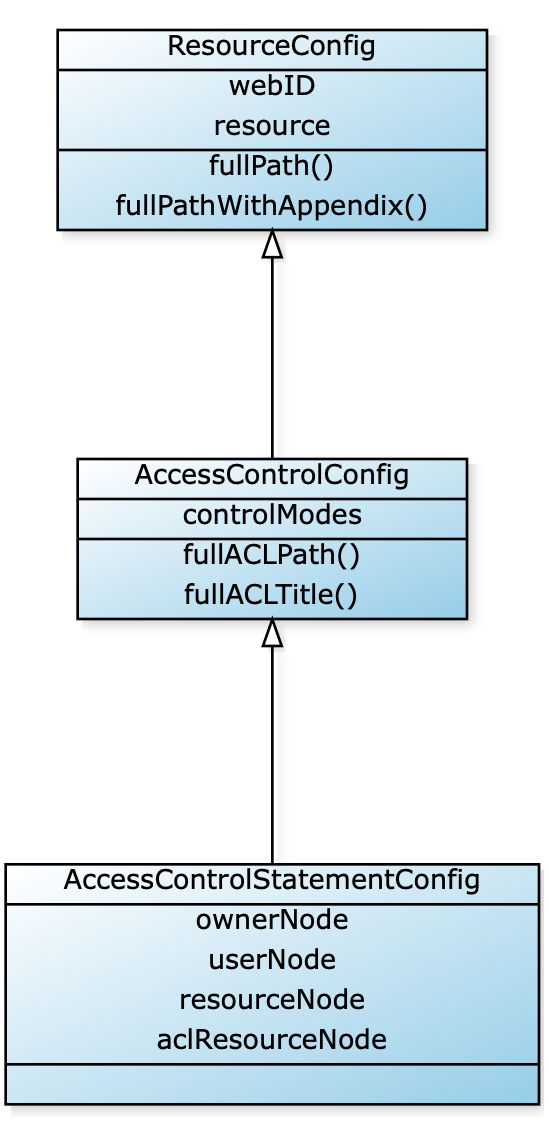
\includegraphics[width=4cm]{lpas_access_control_config_imlementation.png}
\caption{A class diagram generated directly from a TypeScript file, demonstrating implemented \textit{AccessControlConfig} and \textit{AccessControlStatementConfig} extending \textit{ResourceConfig}}
\label{fig:lpas_access_control_config_imlementation}
\end{figure}

\subsubsection{An example on creating an ACL file for a \solid{} resource}

The example below demonstrated a simple use case on how \lpas{} package can be used to create an ACL file for a \solid{} resource using the \textit{FileManager} abstraction. 

\begin{listing}[H]    
\begin{minted}[breaklines,frame=single,framerule=1pt,bgcolor=LightGray]{javascript}
const configurationsAclResourceConfig: AccessControlConfig = new AccessControlConfig(
  {
    ...configurationsFolderConfig.resource,
    isPublic: true
  },
  [AccessControlNamespace.Read, AccessControlNamespace.Write],
  webId
);

const response = await StorageFileManager.updateACL(
  configurationsAclResourceConfig
);
\end{minted}
\caption{An example ES6 code on creating ACL files for \solid{} resource in \lpa{} frontend} 
\label{lst:acl_creation_lpa_example}
\end{listing}

In this case, a folder resource is expressed as a \textit{ResourceConfig} class instance under \textit{configurationsFolderConfig} constant and \textit{configurationsAclResourceConfig} constant is created based on it to express and ACL file. Using the ES6 \texttt{spread} operator we populate the description of the folder resource as follows '\texttt{...configurationsFolderConfig.resource}'. Afterwards, the access control modes are supplied in an array giving the ability to \textit{Read} and \textit{Write} to that resource to anyone by default. In the last step the specify the webId of the owner of the resource and the ACL file to be created and supply the constructed \textit{AccessControlConfig} into \textit{updateACL()} method that is demonstrated in detail on this sequence \autoref{fig:lps_acl_update_flow}.

To sum up, the section provided an overview of three main abstractions inside \lpas{} package. The \textit{AuthenticationManager} used as a main class to deal with WebID based authentications for \lpa{} platform. The \textit{FileManager}, responsible for managing all HTTP requests to manipulate resources in a \solid{} resource. \textit{AccessControlManager} abstraction that significantly simplified the interactions with \solid{} inside \lpa{} frontend significantly and gave an ability to implement more advanced access control related features to configure the published \lpa{} visualizers. This will be demonstrated in detail in \autoref{sssec:lpas_storage_frontend_implementation}. The consequitive section will describe the \lpas{} Ontology originally described in \autoref{fig:lps_acl_update_flow}, its implementation and hosting.

\section{Hosting Storage Ontology}
\label{ssec:storage_ontology_implementation}

This section is going to continue the details on implementation of the \lpas{} ontology, firstly described in \autoref{ssec:lpas_application_ontology_arch}. As mentioned earlier, the intent to design the ontology was to utilize the benefits of \solid{} better and the ways in which every entity is represented as an RDF resource.

\begin{figure}[h]
\centering
\fcolorbox{black}{white}{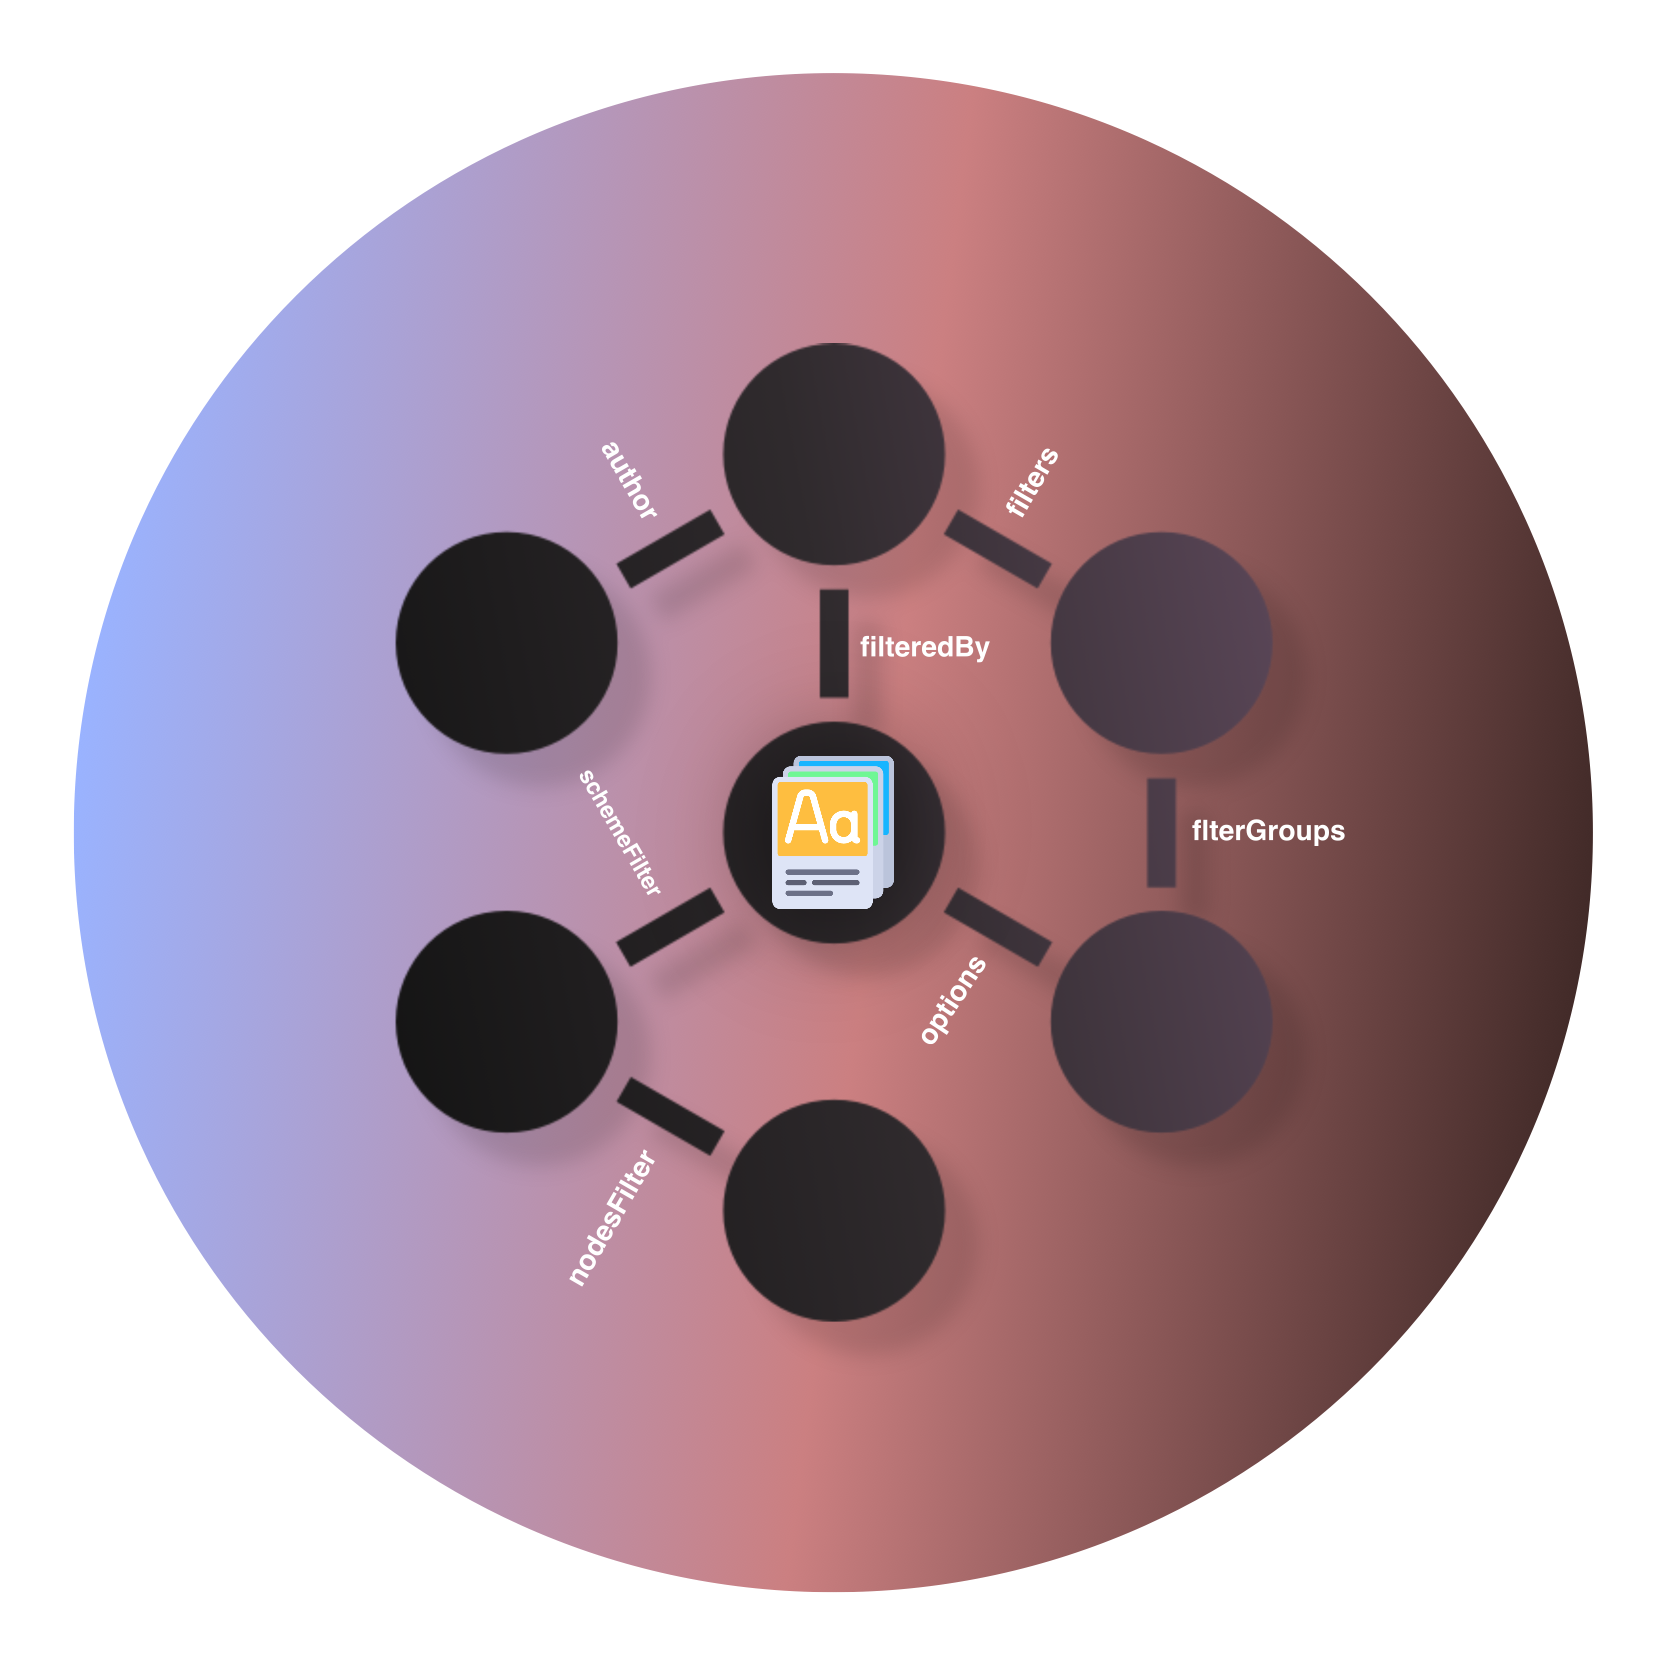
\includegraphics[width=0.4\linewidth]{lpa_ontology_logo.png}}
\caption{Official \lpas{} Ontology logo designed by author.}
\label{fig:lpa_ontology_logo}
\end{figure}

The ontology itself was implemented using a set of open-source tools that will be described in the first part of this section. 

\subsection{Preliminaries}

Two open-source frameworks were used to implement and publish the \lpas{} ontology:
\begin{itemize}
    \item \texttt{Protégé} is an open-source ontology editing framework developed at Stanford University and written in Java programming language \cite{protege}. It provides an intuitive graphical user interface for defining and developing ontologies. The version of the software used at the moment of implementing the ontology is \texttt{v5.5.0}.
    \item \texttt{Ontoology}, is an open-source software solution for collaborative development of ontologies on GitHub \cite{ontoology}. However, in the scope of implementing \lpas{} ontology, it was mainly chosen for its additional features, such as an ability to publish ontologies under permanent \texttt{w3id.org} URL, an ability to host the ontology as a static HTML webpage under GitHub Pages. 
\end{itemize}

\begin{figure}[h]
\centering
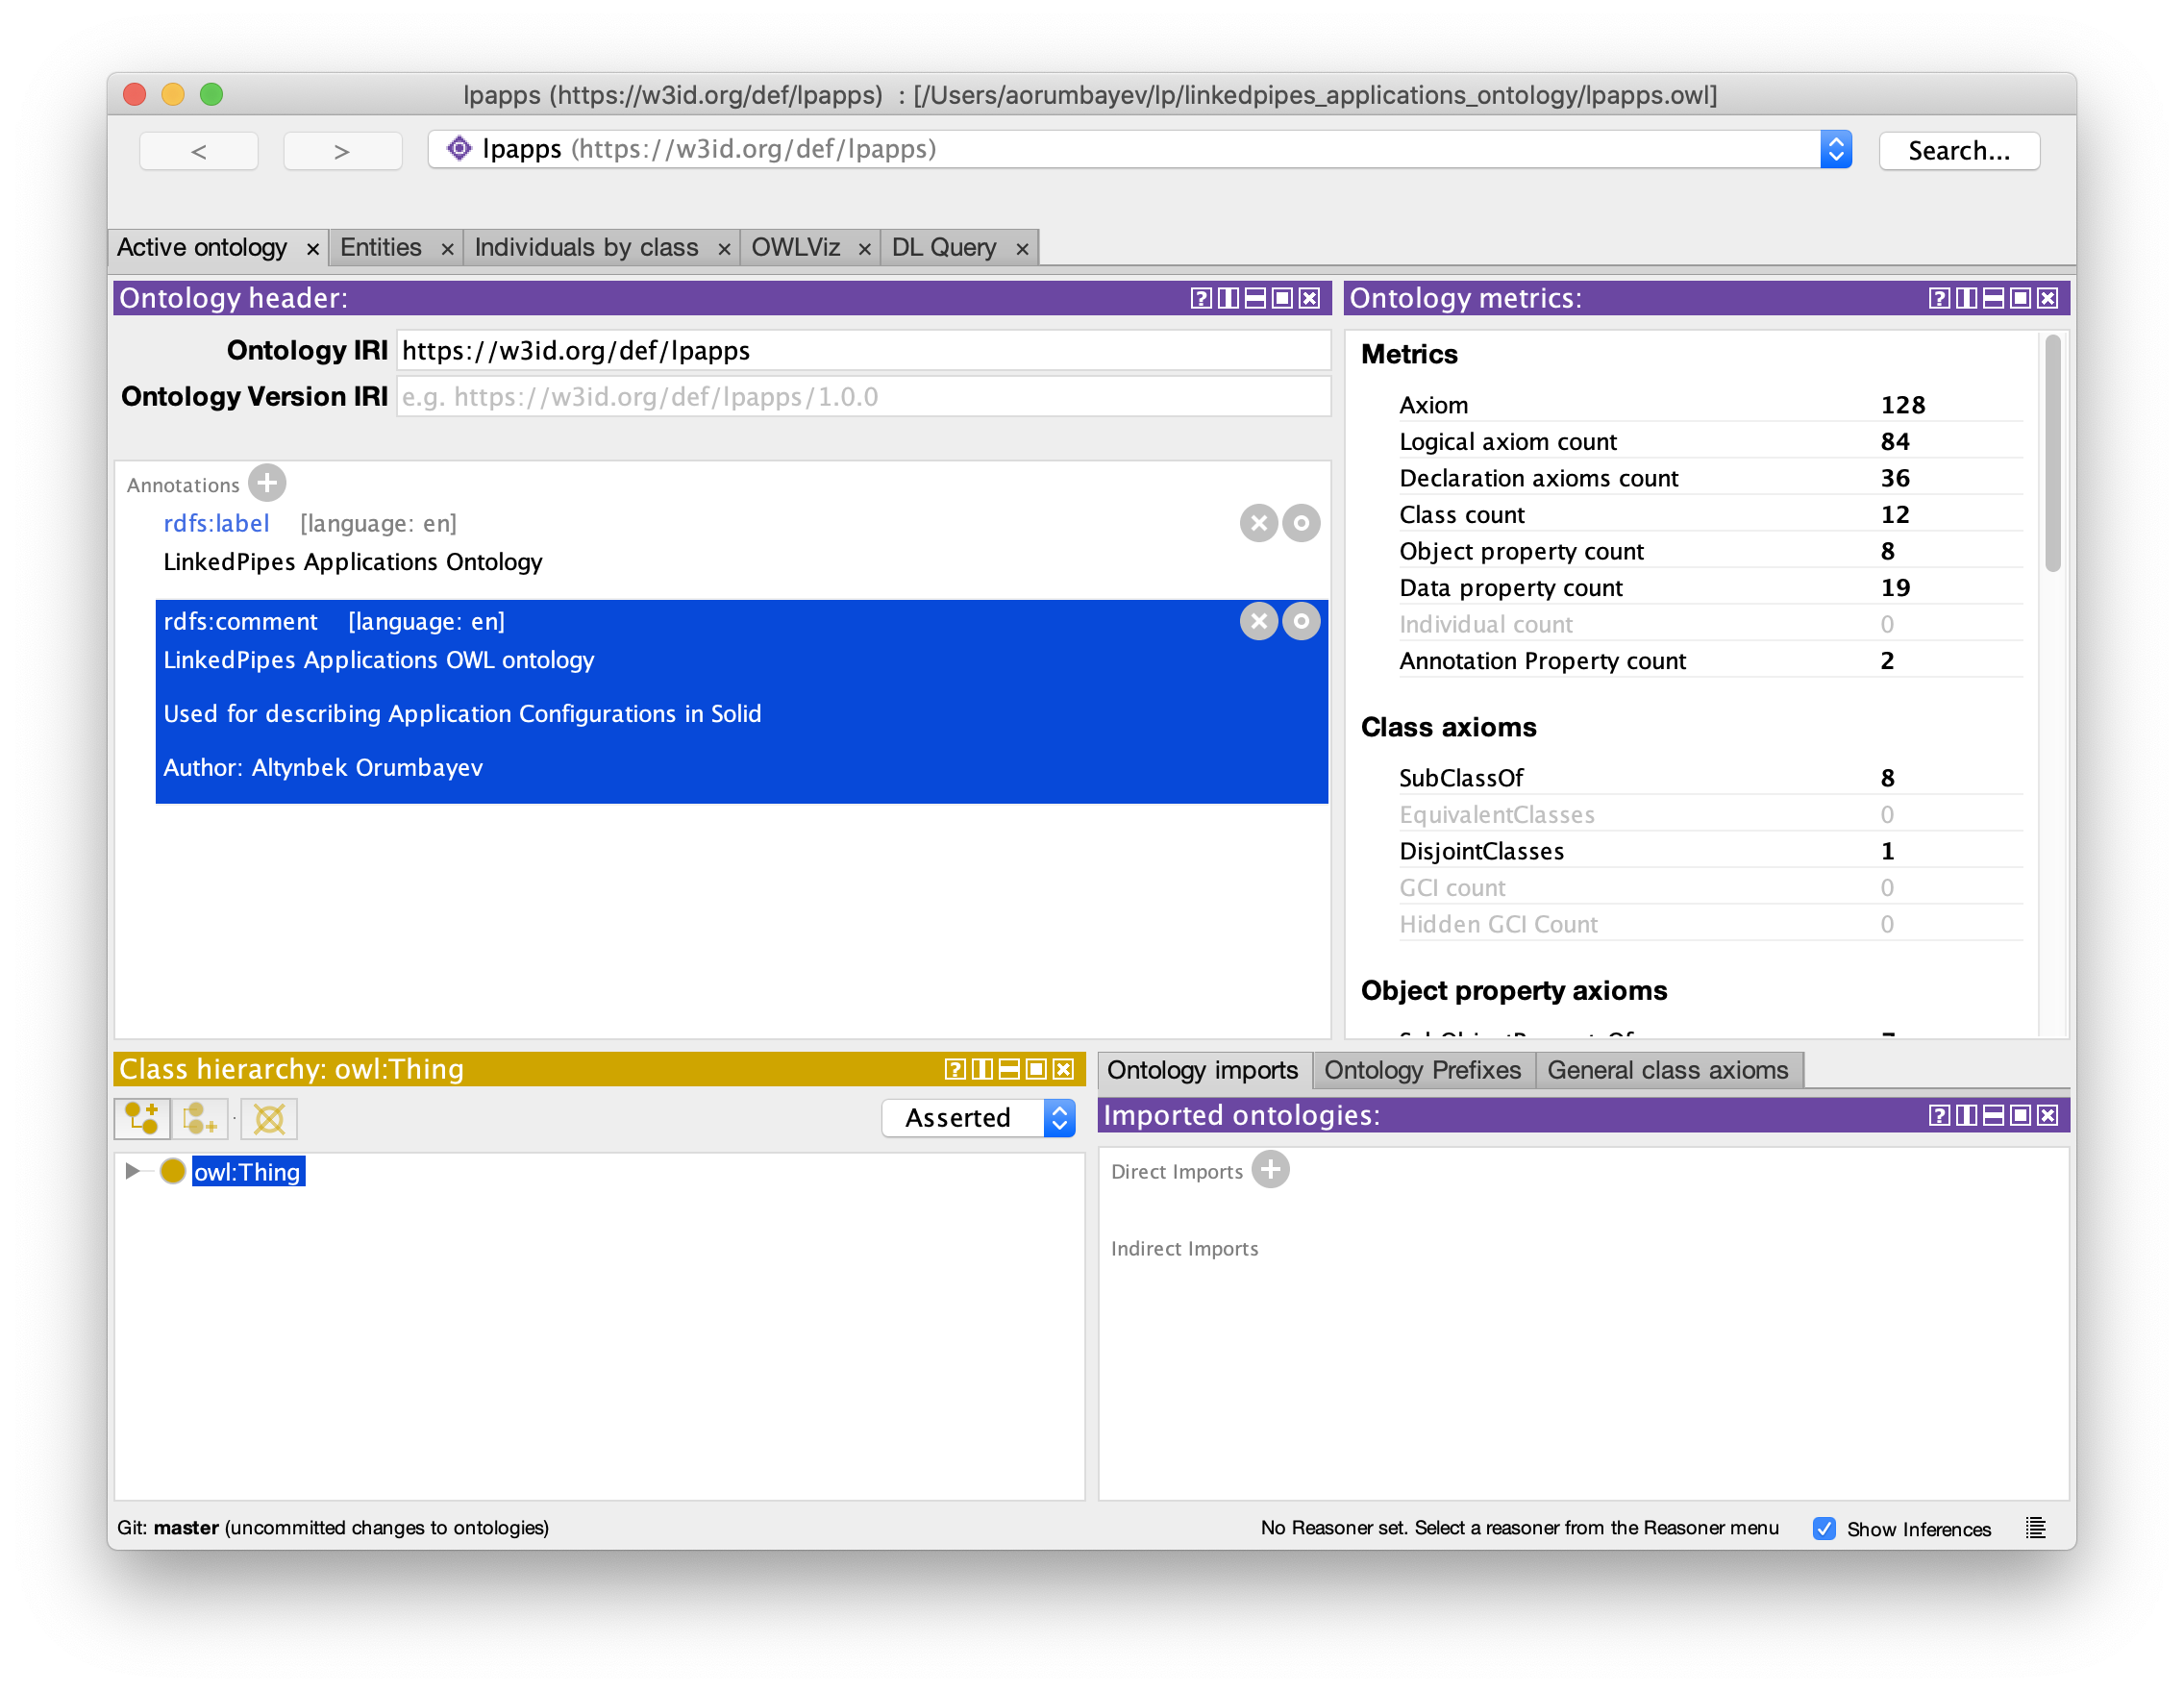
\includegraphics[width=12cm]{misc_ontology_visualizer.png}
\caption{Example UI of \texttt{Protégé} ontology editor at \textit{Active Ontology} tab.}
\label{fig:misc_ontology_visualizer}
\end{figure}

\subsection{Using \texttt{Protégé}}

After defining the main entities and designing the hierarchical structure of the ontology in \autoref{ssec:lpas_application_ontology_arch}, the ontology was implemented using \texttt{Protégé} ontology editor. The editor allows defining the ontology entities by specifying them under:
\begin{itemize}
    \item \textit{Classes}, tab represents the \textit{asserted} and \textit{inferred} class hierarchies as a tree, where each node represents a particular class. The \textit{asserted} class view is a default and primary navigation device for browsing class hierarchies in \textit{Protégé}, the \textit{inferred} classes view on the other hand differs from \textit{asserted} by requiring a reasoner to be setup to render the complete hierarchy view. If no reasoner is provided the \textit{inferred} classes view will be empty.
    \item \textit{Object properties} tab,  represents the graphical user interface to create and define relations between instances of the classes. The view under that tab is similar to the \textit{Classes} tab, the properties are represented as a tree with nodes identifying individual object property. For instance, each \textit{VisualizerConfiguration} can be filtered by a \textit{FilteredConfiguration}, this relation can be expressed by defining an object property calls \textit{filteredBy}.
    \item \textit{Data properties} tab, represents the graphical user to create and define relations between instances of classes and RDF literals or datatypes. For instance, a \textit{VisualizerConfiguration} class has a \textit{backgroundColor} data property which is a \textit{String} datatype. 
\end{itemize}

The resulting ontology created in \texttt{Protégé} was represented as an OWL, which is a format for Web Ontology Language described earlier in \autoref{sssec:using_web_ontology_language}. The following subsection will explain the process of publishing the ontology using the \textit{Ontoology} software. 

\subsection{Using \textit{Ontoology}}

The \textit{Ontoology} itself is an open-source project that can be instantiated and configured manually. It is, however, also available as a standalone running instance \footnote{\url{http://ontoology.linkeddata.es}}. The publishing of the \lpas{} Ontology was done using the available instance instead of manually configuring one, this significantly reduced the development time needed to publish and host the vocabulary to be used in \lpa{} frontend.

The initial configuration or startup guide to \textit{Ontoology} consist of the following steps: 
\begin{enumerate}
    \item \textit{Setup a GitHub repository}, an exported OWL file from \texttt{Protégé} was hosted on a regular public GitHub repository \footnote{\url{https://github.com/aorumbayev/linkedpipes_applications_ontology}} and placed at the root.
    \item \textit{Add repository to Ontoology}, add the repository by name into Ontology, and press \textit{Watch this repo} button. This is pretty much the last step involving any manual work. The following steps are all invoked in an automated fashion, demonstrating the full list of benefits provided by this software.
    \item \textit{Merge initial PR from Ontoology}, once the repository is connected, an automated PR will be opened that will contain a following list of elements:
    \begin{enumerate}
        \item Diagrams, a folder with pre-generated class hierarchy visualizations of the ontology.
        \item Documentation, an automatically generated ontology documentation hosted on GitHub Pages on the same repository, and available at \textit{w3id.org} permanent URL redirecting users to GitHub Pages.
        \item Evaluation report, \textit{Ontoology} generates a report that checks various aspects of the implementation of the ontology, providing hints when, for instance, some parts in the description of an entity is missing.
        \item JSON-LD, an original OWL, the file is automatically converted into a JSON-LD file.  
    \end{enumerate}
\end{enumerate}

\begin{figure}[h]
\centering
\fcolorbox{black}{white}{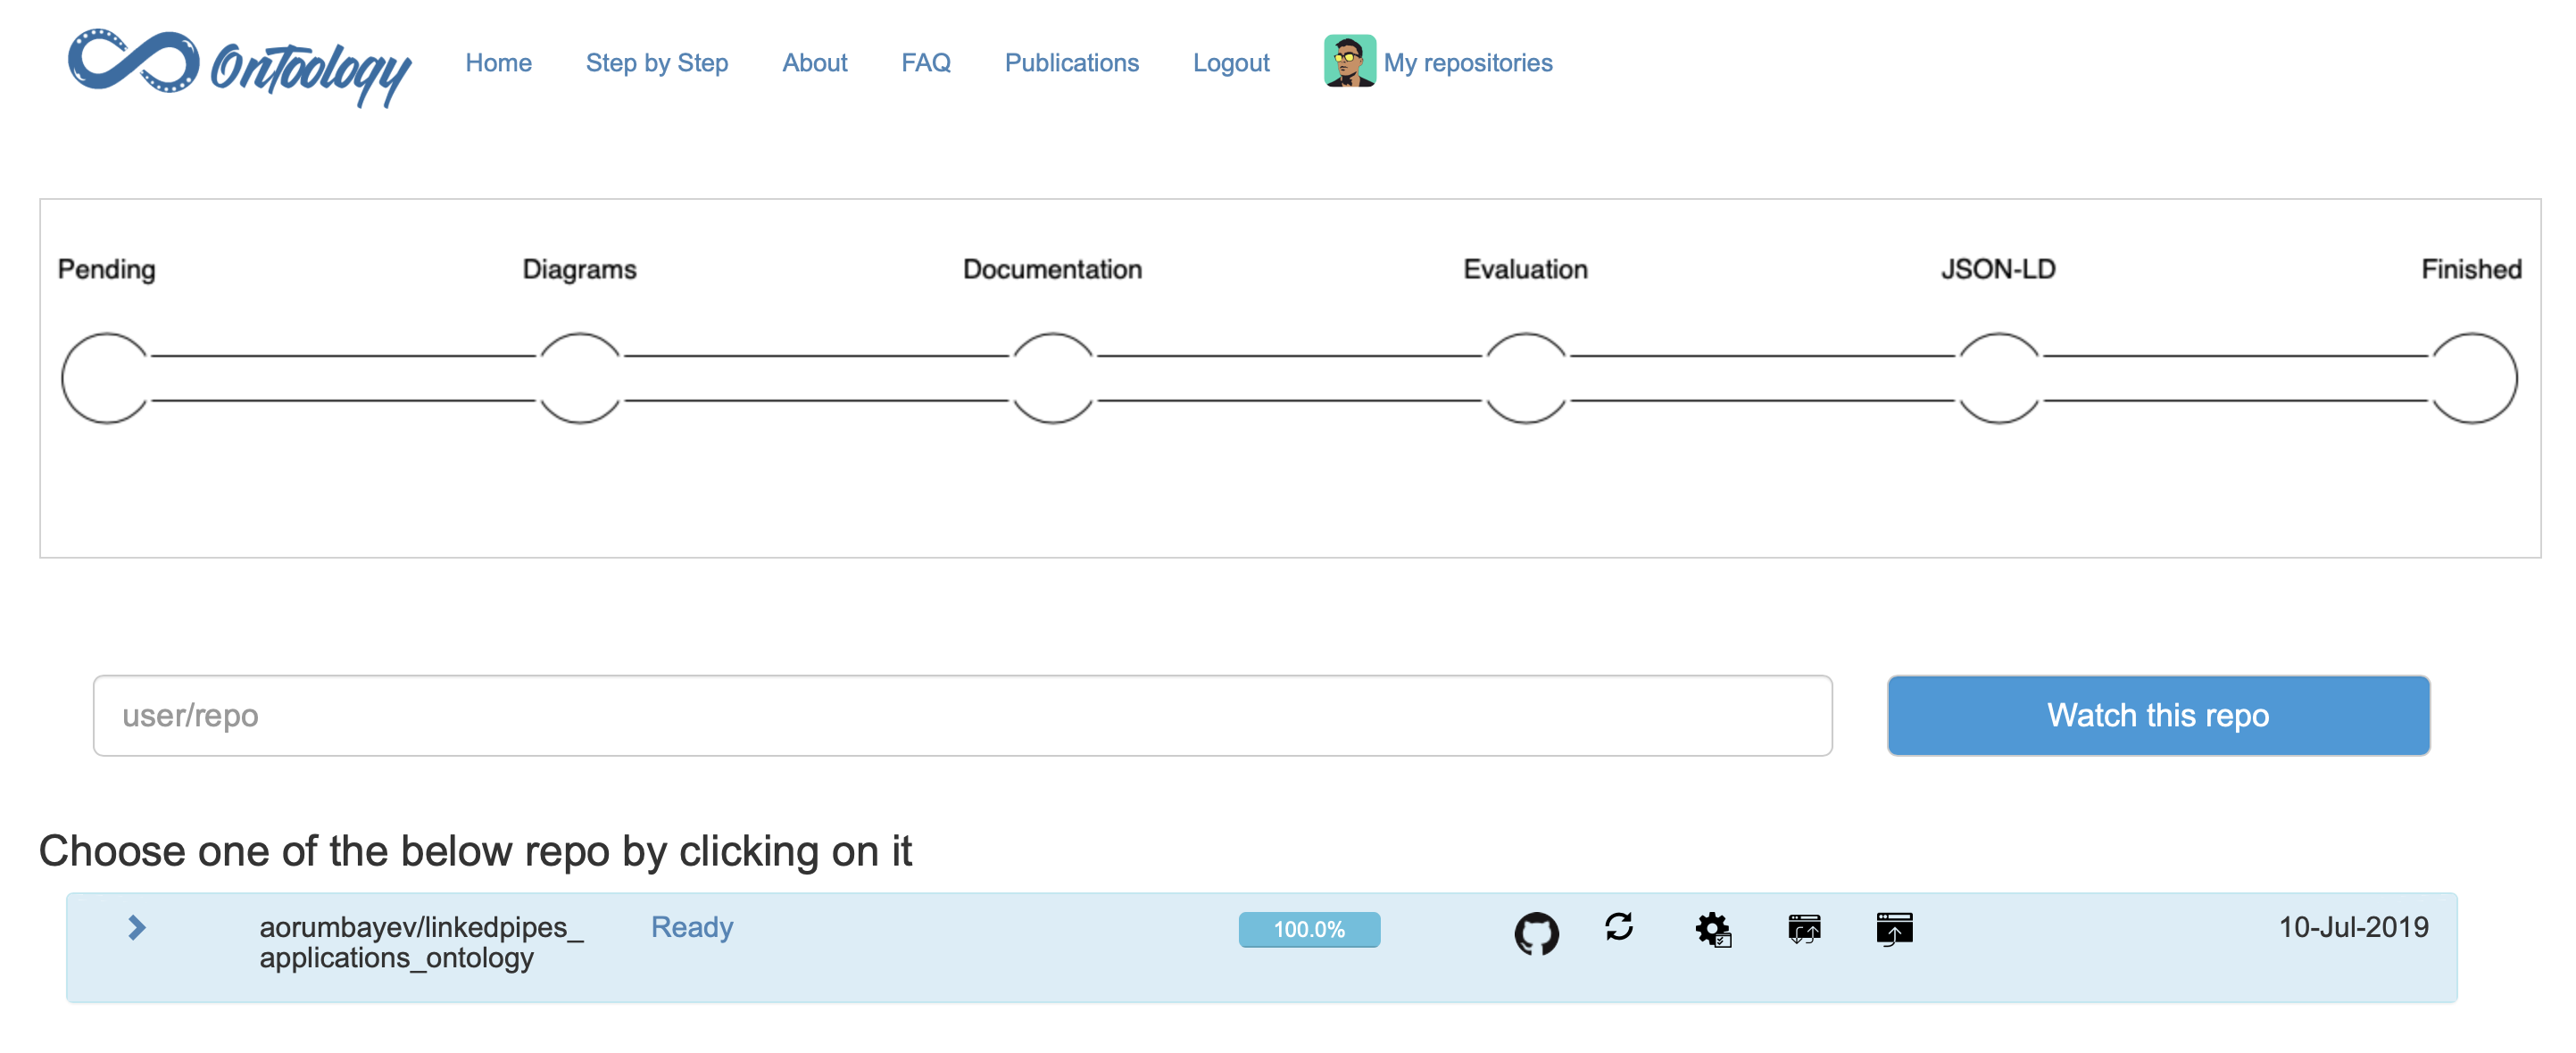
\includegraphics[width=0.8\linewidth]{misc_ontoology_ui.png}}
\caption{UI of Ontoology displaying the processed repository with \lpas{} Ontology.}
\label{fig:misc_ontoology_ui}
\end{figure}

To sum up, the \lpas{} ontology was implemented using two open-source frameworks called \texttt{Protégé} and \texttt{Ontoology}. The first tool was used as an editor to implement the ontology designed in \autoref{ssec:lpas_application_ontology_arch}. The second tool was used to publish and host applications. The detailed documentation will be mentioned in \autoref{chap:num_8} and is also available at \url{http://w3id.org/def/lpapps}. 

\section{Storage Frontend}
\label{sssec:lpas_storage_frontend_implementation}

The following section will continue the \autoref{ssec:lpas_storage_component_design} by providing the details on implementation of individual components interacting with \solid{} POD. 

\subsection{Preliminaries}
\label{sssec:preliminaries_storage_frontend}

To simplify the understanding of this section, it is important to recap the conventions and specifics of \lpa{} frontend implementation by providing some extended details, as they were strictly taken into consideration while developing \lpas{} components inside the \lpa{} frontend codebase.

As mentioned earlier in \autoref{sssec:lpa_preliminaries_component_overview}, the frontend provides a way for the user to interact with the \lpa{}. As demonstrated on the \autoref{fig:lpa_frontend_architecture}, the frontend uses Redux and React as a primary framework for building the components and managing states.

\begin{figure}[h]
\centering
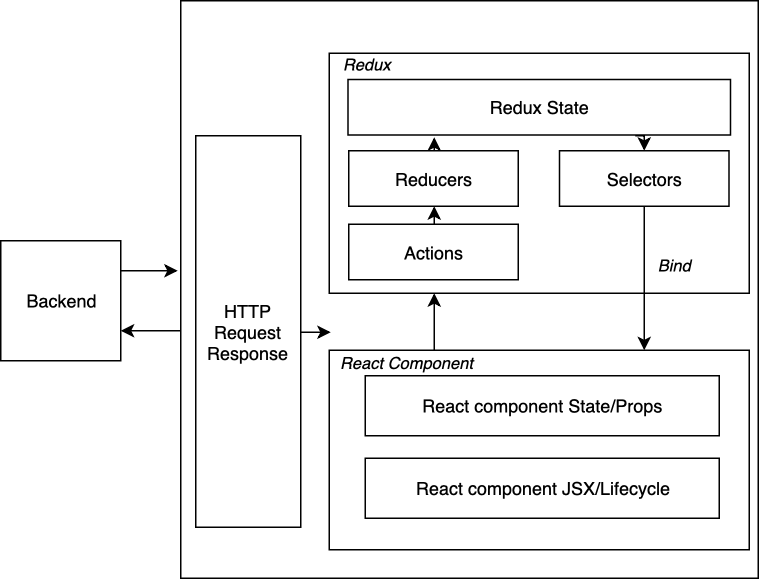
\includegraphics[width=12cm]{lpa_frontend_architecture.png}
\caption{General architecture of Redux store and React components within \emph{frontend}}
\label{fig:lpa_frontend_architecture}
\end{figure}

The main entities displayed on \ref{fig:lpa_frontend_architecture} can be described as follows:

\begin{itemize}
    \item \textit{React Component}, as described in \autoref{ssssec:frontend_preliminaries}, it represents a JavaScript class or function that accepts optional inputs and returns a React element that describes how a section of the User Interface should appear. 
    \item \textit{Redux} as described in \autoref{ssssec:frontend_preliminaries}, it represents an internal state management framework for frontend web frameworks like React.
\end{itemize}

\subsubsection{Frontend code structure}
\label{ssssec:lpa_frontend_code_structure}

The implementation of the \lpa{} frontend is located at the \texttt{src/frontend} path at official \lpa{} repository \footnote{\url{https://github.com/linkedpipes/applications}}  and structured as follows:

\begin{itemize}
    \item \textit{constants} - contains all constants used throughout the frontend component implementation.
    \item \textit{utils} - contains various handy utility classes, variables, and methods.
    \item \textit{ducks} - contains all Redux reducers, actions and selectors. The title \textit{duck} comes from a convention proposed by Erik Rasmussen in \cite{redux_ducks}, it suggests a way to bundle Redux entities into folders that are easier to manage and maintain as they contain reducers, actions, and selectors.
    \item \textit{layouts} - contains a global setup for various components as well as the specification for the MaterialDesign theme used in the project.
    \item \textit{components} - contains all components with JSX file type, visualizers and various UI elements implementations not related to interactions with \solid{}. The JSX is a syntactic extension for JavaScript that adds the ability to combine ES6 syntax with HTML tags.
    \item \textit{containers} - contains complex layouts for specific web-pages of the web app not related to interactions with \solid{}. Each folder is named after the individual webpage. 
    \item \textit{storage} - contains all contributions and implementations made within the scope of \lpas{} project. It has a substructure mimicking the global folder structure to improve code maintainability and signify the difference between implementations of \lpa{} and \lpas{}.
    \item \textit{configuration files and entry points}, contains a set of configuration files at the root, such as linter configurations, the file with global Redux store and a file called \textit{AppRouter}, which is the main controller of the whole frontend since it manages the user sessions and establishes the socket connections with \lpa{} backend.
\end{itemize}

\subsection{Storage folder structure}
\label{sssec:storage_folder_structure}

As mentioned in \autoref{ssssec:lpa_frontend_code_structure}, let us describe the internals of \textit{storage} folder inside \lpa{} frontend codebase. 

\begin{itemize}
    \item \textit{utils} - contains various handy utility classes, variables, and methods for storage specific React Components.
    \item \textit{ducks} - contains all Redux reducers, actions and selectors for storage specific React Components. 
    \item \textit{models} - contains classes representing \textit{VisualizerConfiguration} and other \lpa{} specific classes that did not have to be split into the \lpas{} package.
    \item \textit{components} - contains all components, visualizers and various UI elements implementations not related to interactions with \solid{}.
    \item \textit{containers} - contains complex layouts for storage specific web-pages. Each folder is named after individual webpage.     
    \item \textit{StorageBackend} - represents a class wrapping various utilities on top of basic \lpas{} storage abstractions. The logic related to fetching the \lpa{} configurations is implemented in this file.
    \item \textit{StorageToolbox} - represents a class wrapping the \textit{StorageBackend} utilities into simple methods to be invoked directly from internal methods of Storage React Components. In other words, it serves as a middleware layer between React Components and low level and generic functionality of \lpas{} package abstractions.
    \item \textit{StorageSparqlClient} - a class containing a single generic method that utilises the \textit{fetch()} function from \textit{AuthenticationManager} to submit \texttt{SPARQL} requests modifying certain parameters of \lpa{} configuration RDF files. 
\end{itemize}

\subsection{Authentication View}
\label{sssec:authentication_view_implementation}

This section continues the architecture and mocks provided in \autoref{ssec:lpas_storage_component_design}, and describes the implementation of the React Component in detail.
To comply with conventions of \lpa{} frontend, the webpage is represented by two separate React Components, one of which is stateful and the other is stateless and manages the views only. The implementation is located at \texttt{src\-/frontend\-/containers\-/AuthenticationPage} path on \lpa{} repository. The folder is named after the webpage and consist of:
\begin{itemize}
    \item \textit{AuthenticationContainer}, a file containing the stateful React Component. In other words, it manages local views specific states as well as global states related to Redux.
    \item \textit{AuthenticationComponent}, a file containing implementation of stateless React Component. In other words, it is only responsible for passing the React \textit{props} and rendering simple views.
    \item \textit{SolidProviderComponent}, a file located in a sub-folder called \textit{children}. The component renders the drop-down menu that allows users to pick specific provi\-der from a list of supported \solid{} providers.
\end{itemize}

\begin{listing}[H]    
\begin{minted}[breaklines,frame=single,framerule=1pt,bgcolor=LightGray]{javascript}
const mapStateToProps = state => {
  return {
    webId: state.user.webId
  };
};

export const AuthorizationContainer = connect(mapStateToProps)(Authorization);
\end{minted}
\caption{An example of mapping Redux state to a props of React Container} 
\label{lst:map_state_to_props_example}
\end{listing}

Following that pattern, the \textit{render()} function of \textit{AuthenticationContainer} expects an instance of \textit{AuthenticationComponent} while passing both internal and Redux state as props to it. The global structure of all Redux states in \lpa{} is too specific to be described within the scope of the \lpas{} project. However, examples of states relevant to Authentication View are going to be provided. For instance, the code example at \autoref{lst:map_state_to_props_example} demonstrates a typical example of an operation that maps the Redux states to \textit{props} of a React Component, in this case, we are mapping the global \textit{webID} value that is used by React Router to identify whether user is authenticated and can render the dashboard or should be redirected back to the screen. As it was mentioned earlier in \autoref{ssssec:lpa_frontend_code_structure} and \autoref{sssec:authentication_manager_implementation}, the \textit{AppRouter} is one of the main entry points to the frontend web app, and it directly utilizes both \textit{AuthenticationManager} abstraction from Authentication React component. An example code on \autoref{lst:track_session_example} demonstrates a code snippet from \textit{AppRouter} that is invoked every time the user session is being authenticated, or user is logging out.

\begin{listing}[H]    
\begin{minted}[breaklines,frame=single,framerule=1pt,bgcolor=LightGray]{javascript}
AuthenticationManager.trackSession(session => {
  if (session) {
     handleSetUserWebId(session.webId);

     self.startSocketListeners();
     ...
  }
})
\end{minted}
\caption{An example of \textit{trackSession()} callback listening for changes in authentication state} 
\label{lst:track_session_example}
\end{listing}

The User Interface strictly follows initial mock design demonstrated at \autoref{fig:lpas_authenticate_mock}. User has an ability to perform authentication either by choosing an individual \solid{} provider or use a supply his WebID directly if his \solid{} provider is not available in the list of default providers. At the moment of writing this part, the project provides support for \texttt{inrupt.net} \footnote{\url{https://inrupt.net}}, \texttt{solid.community} \footnote{\url{https://solid.community}} and self-hosted provider made specifically for LinkedPipes available at \textit{lpapps.co} \footnote{\url{https://lpapps.co:8443}}. After performing the authentication use is redirected into the Dashboard webpage of \lpa{} frontend.

\subsubsection{Overview of states and methods}

As general details on the structure of the implementation are defined now, let us dive deeper into the description of main states and functions of Authentication View components. As \textit{AuthenticationComponent} is a stateless React component, it is sufficient to provide definitions for states and methods in \textit{AuthenticationContainer} as this represents the main functionality of the whole webpage. The states can be described as follows:
\begin{itemize}
    \item \textit{webIdFieldValue}, a \texttt{string} value holding input at the \textit{textfield} for supplying WebID value.
    \item \textit{withWebIdStatus}, a \texttt{boolean} value representing the current input state and whether is chosen to use available providers or entered his WebID manually.
    \item \textit{session}, an \texttt{object} representing current session returned from \textit{AuthenticationManager} abstraction.
    \item \textit{providerTitle}, a \texttt{string} value holding the title of selected provider. This is needed to be supplied into \textit{login()} method of \textit{AuthenticationManager} abstraction that invokes the \texttt{solid-auth-client} library.  
\end{itemize}

The set of methods inside the \textit{AuthenticationComponent} class can be described as follows:
\begin{itemize}
    \item \textit{handleProviderChange()} a methods that is passed as a \texttt{prop} to \textit{AuthenticationComponent}, and invoked every time user selects or update his selection of default providers.
    \item \textit{handleSignIn} a method that is invoked when is pressing the \textit{Authenticate} button, this redirects a call to \textit{AuthenticationManager} abstraction that initiates the sequence flow described at \autoref{fig:lps_authentication_sequence_diagram}.
    \item \textit{handleWebIdFieldChange} a method invoked when user inputs or modifies the input at the \textit{textfield} used for WebID.
    \item \textit{isWebIdValid} a method that uses \textit{regex} to validate whether provided WebID is in valid format.
    \item \textit{onSetWithWebId} a method invoked when the \textit{withWebIdStatus} status is being changed.  
\end{itemize}

The final rendered UI of this implementation will be provided in the of this chapter under \autoref{ssec:overview_of_implemented_requirements}, where a detailed overview of a final implementation satisfying each of the original \lpa{} requirements are provided.

\subsection{Storage Dashboard}
\label{sssec:storage_dashboard_implementation}

The Storage Dashboard webpage described at \autoref{sssec:architecture_storage_dashboard} was a challenging component to implement. To simplify the understanding of the structure in which components and containers are invoked, the \autoref{fig:storage_dashboard_implementation_diagram} is provided. The components demonstrated on diagram follow the usual pattern of splitting React Components into stateful and stateless and can be described as follows:
\begin{itemize}
    \item \textit{StoragePageController} is a root React component that wraps both individual and shared application views. It stores states representing the tab index and depending on the selected index it switches the components to be rendered in \textit{render()} function.
    \item \textit{StorageAppsBrowser*}, both container and component represent a view that fetches and displays \lpa{} configurations. The stateless part relies on the \textit{Grid} layout system from \texttt{MaterialUI} framework.
    \item \textit{StorageSharedAppsBrowser*}, both container and component represent a view that fetches and displays \lpa{} configurations that were shared with the User. The stateless part relies on the \textit{Grid} layout system from \texttt{MaterialUI} framework.
    \item \textit{StorageAppsBrowserCardComponent} is a child component that represents a reusable card representing an individual \lpa{} configuration in a grid of cards.
\end{itemize}

The user interface is inspired by the mock at \autoref{fig:lpas_ui_dashboard_mock}. However, it is more refined and optimized to fit the general style of \lpa{} frontend. Similar to the Authentication view, the final rendered UI of this implementation will be provided at the end of this chapter under \autoref{ssec:overview_of_implemented_requirements}.

\begin{figure}[h]
\centering
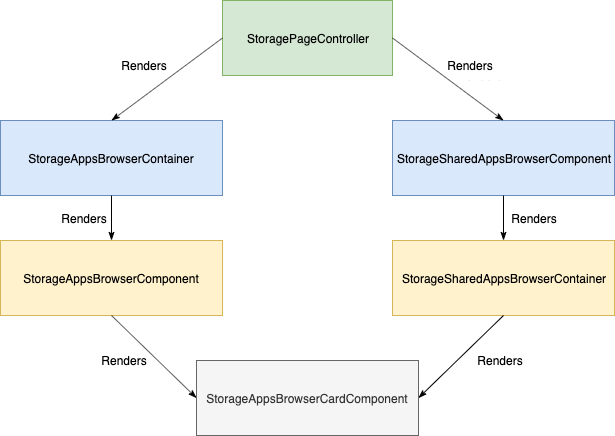
\includegraphics[width=10cm]{storage_dashboard_implementation_diagram.png}
\caption{Diagram representing the chain of \textit{render()} method invocations among components representing Storage Dashboard.}
\label{fig:storage_dashboard_implementation_diagram}
\end{figure}

\subsubsection{Overview of main functionality}

In contrast with Authentication View, the structure of sub-components is rather complex to describe in detail. Therefore a set of primary states and methods responsible for the core functionality of the webpage will be described instead.

In general both \textit{StorageAppsBrowser*} and \textit{StorageSharedAppsBrowser*} components and containers share similar states and functions the only difference is the way stored \lpa{} configurations are fetched. The fetching itself is done by invoking the corresponding methods called \textit{getAppConfigurationsMetadata()} and \textit{getSharedApplicationsMetadata()} methods from \textit{StorageToolbox} class. In general, the \textit{StorageToolbox} invokes lower-level wrappers in \textit{StorageBackend} that utilize the \texttt{rdflib} library from \lpas{} package and converts the RDF resource representing the \lpa{} configuration into a JavaScript object that is processed by \textit{StorageAppsBrowserCardComponent} view.

\subsection{Storage Control Panel}
\label{sssec:storage_control_panel_implementation}

The Storage Control Panel is rather a simple set of React Components that heavily rely on \textit{FileManager} abstraction from \lpas{} package. As initially described in \autoref{sssec:architecture_storage_control_panel}, the functionality should provide user options to perform basic operations with the root folder for all \lpa{} configurations in his \solid{} POD. Those operations include changing the title of the root folder, moving within the pod, or copying within the pod. The implementation consist of the following classes:
\begin{itemize}
    \item \textit{StorageAccessControlDialog} is a stateful React Component based on \textit{Dialog} Component from \textit{Material UI} framework. Due to simplicity of the elements to be rendered, it did not require splitting into stateful and stateless components.
    \item \textit{SettingsPageComponent} is a stateless React Component that renders the simple label with the current path to the root storage folder in \textit{Solid} and a simple button to change it by invoking the \textit{StorageAccessControlDialog}.
    \item \textit{SettingsPageContainer} is a stateful React Component that serves to connect the \textit{StorageAccessControlDialog} and \textit{SettingsPageComponent}.
\end{itemize}

\subsubsection{Overview of main functionality}

In general, the main functionality is located in the \textit{StorageAccessControlDialog} class, it strictly follows the mock at \autoref{fig:lpas_change_folder_mock} and can be described as follows:
\begin{itemize}
    \item \textit{handleFolderConfirm()} a method invoked when user clicks on \textit{Update} button. The component then invokes the \textit{StorageToolbox} class that communicates with \textit{FileManager} abstraction in \lpas{} package. For more detailed description of how \lpas{} package performs the \texttt{CRUD} operations on resources in \solid{} PODs refer back to \autoref{chap:num_4}.
    \item \textit{handleFolderCopy()} a method invoked when user clicks on \textit{Copy} button. The rest is similar to \textit{handleFolderConfirm()} where \textit{StorageToolbox} is invoked and it communicates with \textit{FileManager} abstraction in \lpas{} package. 
    \item \textit{handleFolderMove()} a method invoked when user clicks on \textit{Move} button. The proceeding invocation chain is identical to methods before.
\end{itemize}

The final rendered UI of this implementation will be provided in \autoref{ssec:overview_of_implemented_requirements}, demonstrating the \textit{StorageAccessControlDialog}, \textit{SettingsPageComponent} and \textit{SettingsPageContainer}.

\section{Implemented functional requirements}
\label{ssec:overview_of_implemented_requirements}

This section will iterate over the requirements from \lpa{} stated in \autoref{chap:num_3}, and demonstrate how each of the functional requirement was implemented by classes and abstractions described in previous sections of this chapter. For requirements that directly involved the implementation of React components, detailed renders of final User Interfaces will be provided. It is important to note that this section offers the implementation overview of all stated functional requirements defined in \autoref{ssec:functional_requirements}.

\subsection{User Authentication}

To recap the User Authentication functional requirement, the user of the platform should be able to register an account in the application, log in, and log out. To fulfill the requirement, the Authentication View component described at \autoref{chap:num_1} was implemented. The final render on \autoref{fig:lpa_login_webpage} provides an intuitive User Interface that allows authentication by selecting a default \solid{} provider, as demonstrated on \autoref{fig:lpa_login_webpage_dropdown} or by specifying the WebID for authentication directly. The \textit{Learn more about WebID, and SOLID} button serves as a guide for users new to \solid{}, clicking the button will get them redirected to the official \texttt{inrupt} website. 

\begin{figure}[hbt]
\minipage{0.5\textwidth}
  \fcolorbox{black}{white}{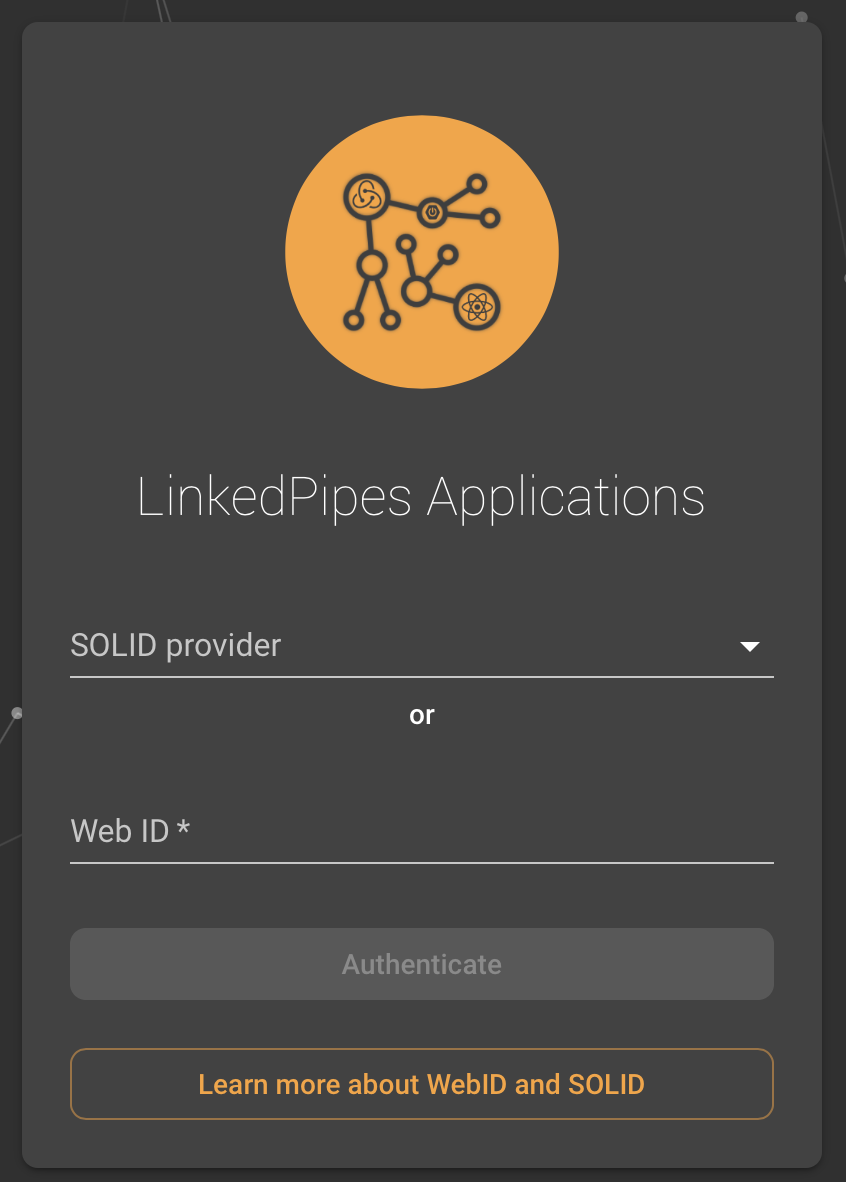
\includegraphics[width=0.8\linewidth]{lpa_login_webpage.png}}
  \caption{The final render of an Authentication View webpage}
  \label{fig:lpa_login_webpage}
\endminipage\hfill
\minipage{0.5\textwidth}
  \fcolorbox{black}{white}{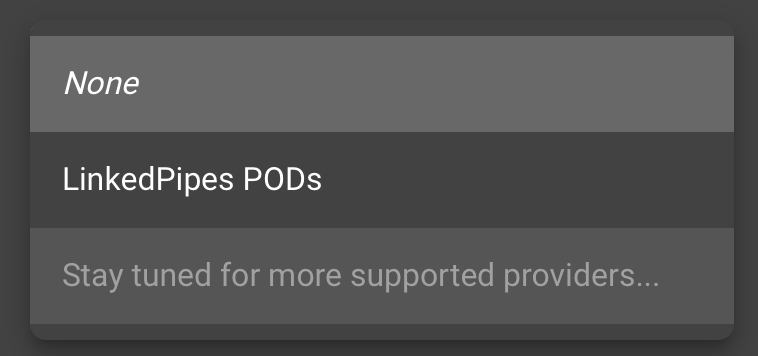
\includegraphics[width=0.8\linewidth]{lpa_login_webpage_dropdown.png}}
  \caption{And example of the \textit{providers} dropdown in expanded state.}
  \label{fig:lpa_login_webpage_dropdown}
\endminipage\hfill
\end{figure}

After user provides the authentication inputs and clicks on \textit{Authenticate} button, the default \solid{} server authentication popup will appear as demonstrated on \autoref{fig:solid_login_webpage} and \autoref{fig:solid_register_webpage}. Depending on whether user has a WebID and a \solid{} POD or if user selected the authentication option using default providers he will be given an option to either \textit{Login} or \textit{Register} on specified \solid{} server. 

\begin{figure}[hbt]
\minipage{0.6\textwidth}
  \fcolorbox{black}{white}{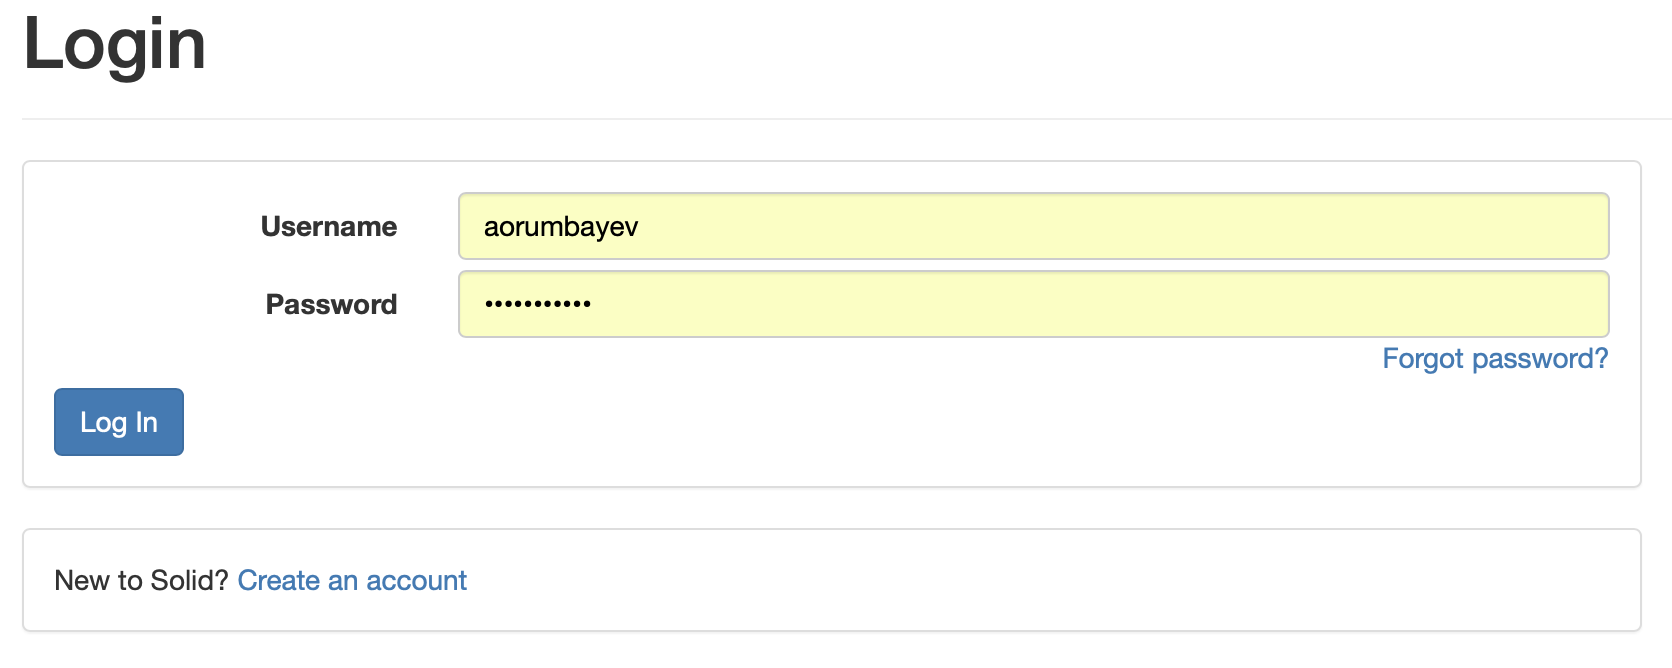
\includegraphics[width=0.8\linewidth]{solid_login_webpage.png}}
  \caption{Example of a login popup provided by \solid{} server.}
  \label{fig:solid_login_webpage}
\endminipage\hfill
\minipage{0.3\textwidth}
  \fcolorbox{black}{white}{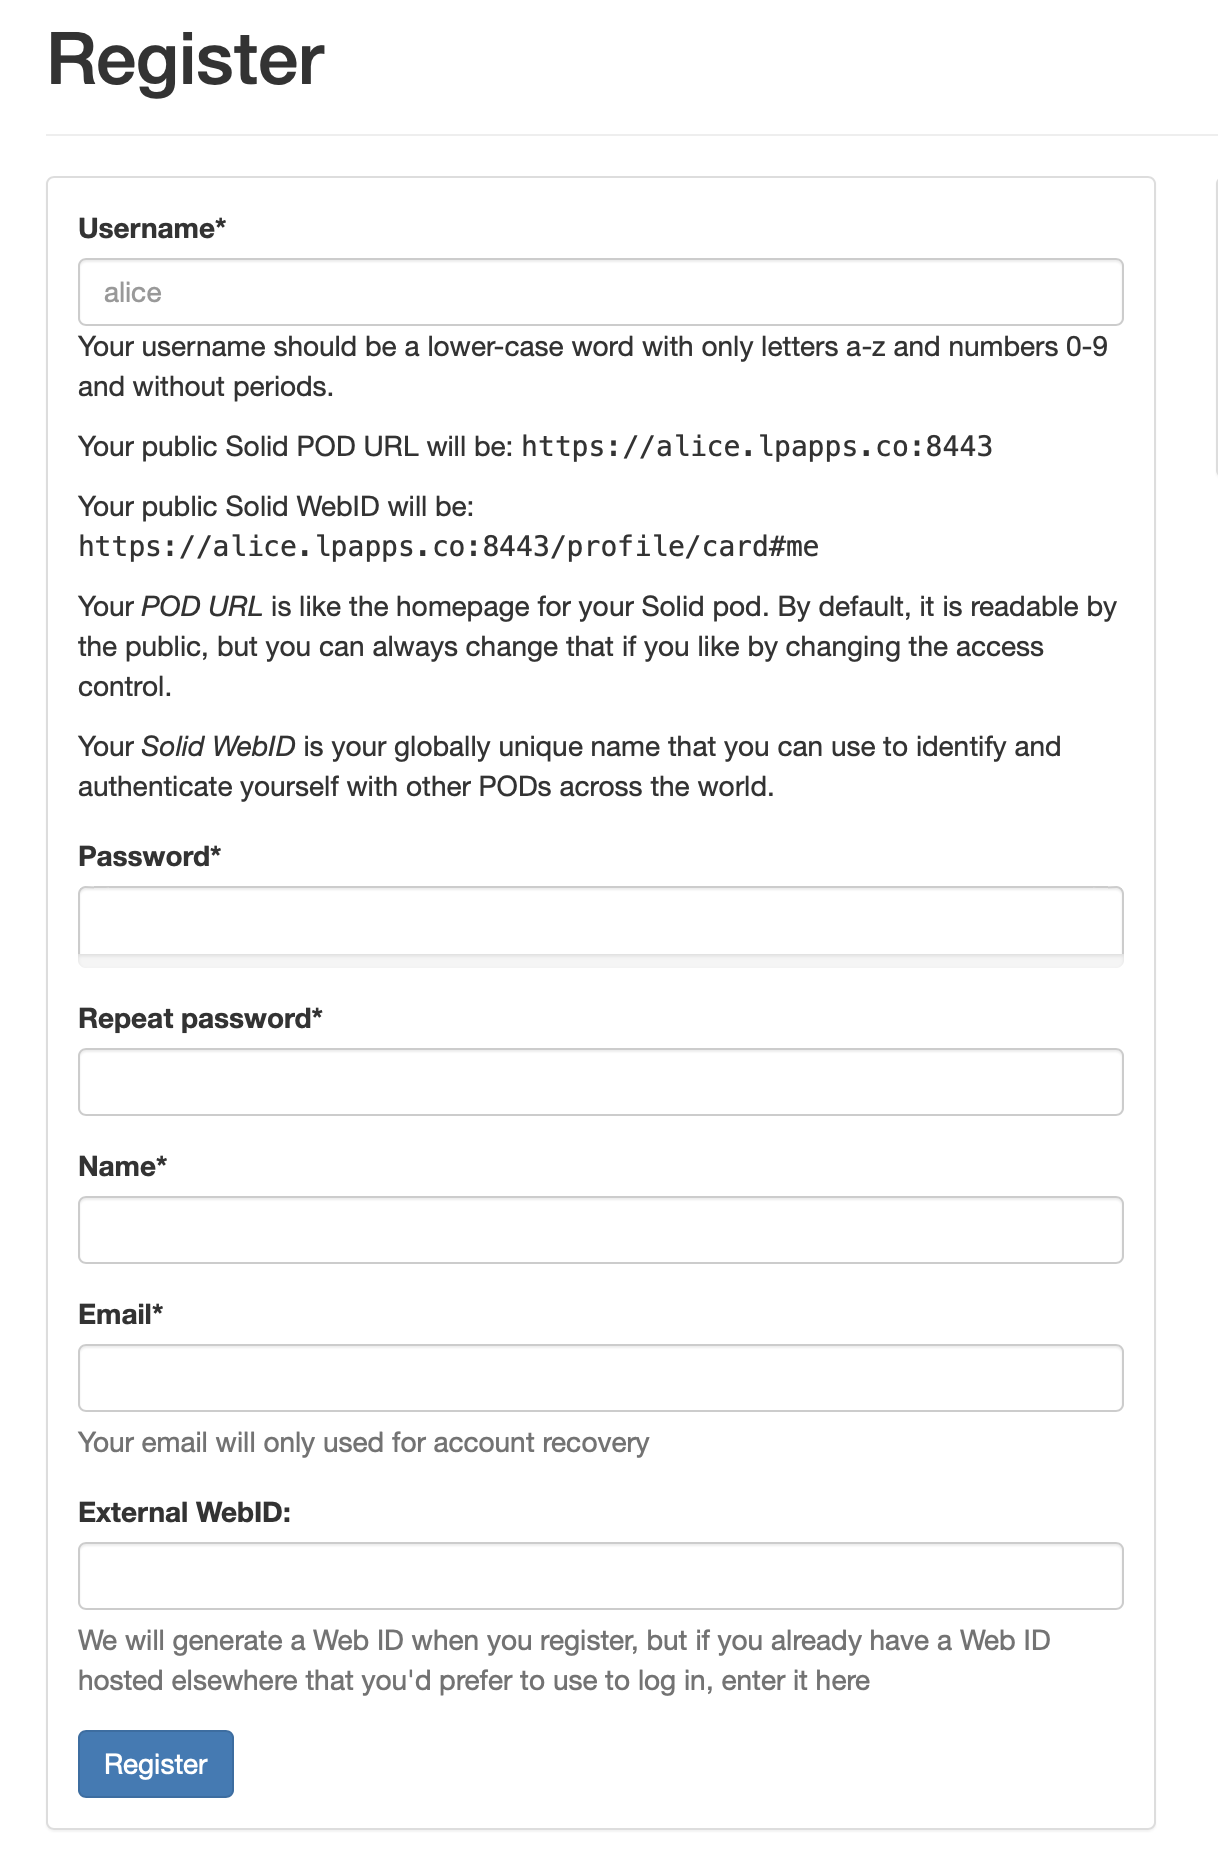
\includegraphics[width=0.8\linewidth]{solid_register_webpage.png}}
  \caption{Example of a register popup provided by \solid{} server}
  \label{fig:solid_register_webpage}
\endminipage\hfill
\end{figure}

The \textit{logout} functionality is available under several components in \lpa{}. Those can be described as follows:
\begin{itemize}
    \item \textit{User Profile Page}, this page is located under settings tab in \lpa{} platform. The intent is to provide the information about the current user name and his WebID under which the authentication was performed. It also provides buttons to either \textit{Reset Password} or \textit{Logout} from the platform.
    \item \textit{Logout toolbar item}, this is a toolbar element always available in the top right corner of the platform. Clicking on the button invokes the \textit{logout}, and the user is redirected back to the Authentication View webpage.
\end{itemize}

\begin{figure}[hbt]
\minipage{0.5\textwidth}
  \fcolorbox{black}{white}{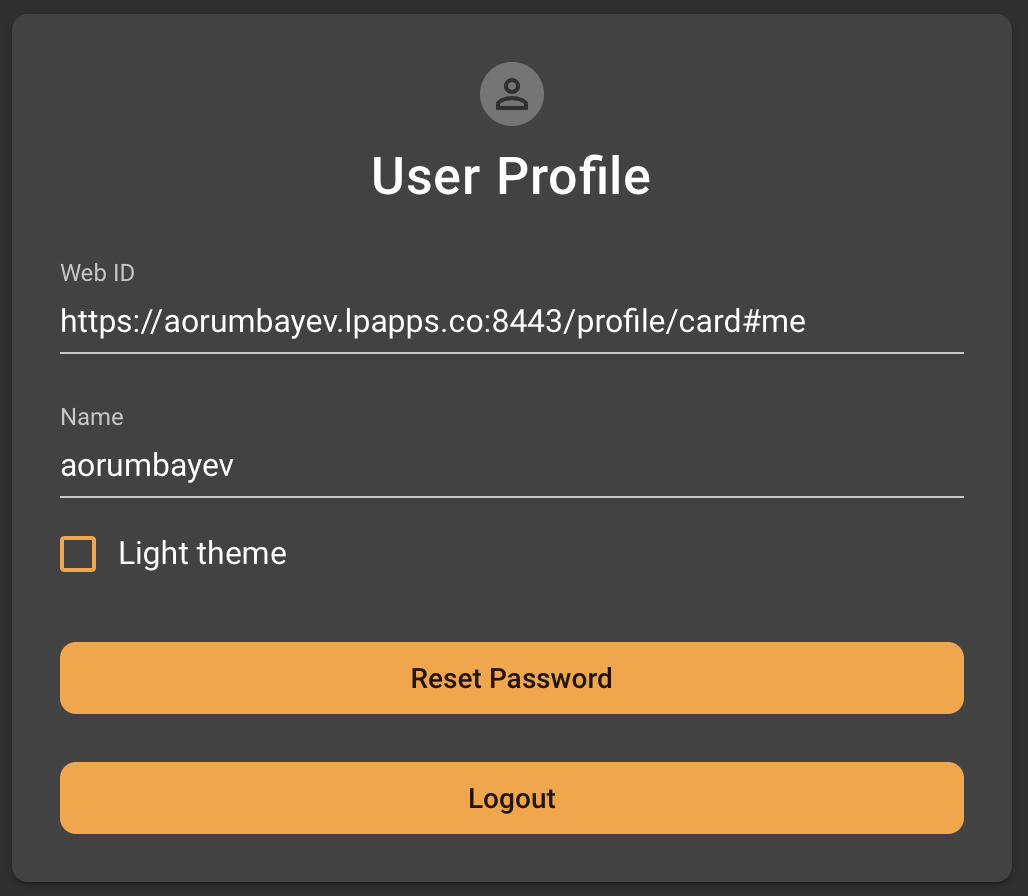
\includegraphics[width=0.8\linewidth]{lpa_user_profile_page.png}}
  \caption{The User Profile webpage with options to reset or logout from \solid{} provider.}
  \label{fig:solid_user_profile_login_webpage}
\endminipage\hfill
\minipage{0.4\textwidth}
  \fcolorbox{black}{white}{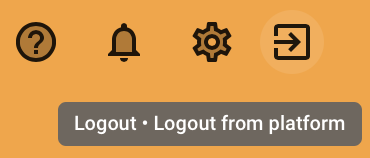
\includegraphics[width=0.8\linewidth]{lpa_user_profile_page_logout.png}}
  \caption{The global control toolbar of \lpa{} platform. The logout button allows to quickly logout from authenticated \solid{} provider.}
  \label{fig:solid_toolbar_logout}
\endminipage\hfill
\end{figure}

\subsection{Create, Store and Publish Application}

The Create and Publish Application requirements are one of the core requirements that are both applicable to \lpas{} and \lpa{} frontend itself. The separation of code contributions to both \lpa{} and \lpas{} was a challenging task. From the standpoint of \lpas{}, an application is created when its configuration is stored as an RDF resource inside \solid{} POD. Having a stored configuration also implies that the application described by this configuration is published because the URI to configuration inside the POD is publicly available by default. In other words, storing creation and publishing of the application are closely related requirements that are easier to cover at once. The section will also focus on the parts of these functional requirements that directly related to interactions with \solid{} server. Additionally, It is important to mention that there is no actual application being stored in the \solid{} pod, the app itself is a React Component that is re-rendered from scratch based on the \lpa{} configuration that is loaded from the storage. 

The \lpa{} platform has a process called \textit{Application data preparation workflow}. It consists of four steps during which a user of the platform provides data sources to visualize, and if successful, the \lpa{} redirects him to a \textit{Create Application} webpage. At this point, the platform assembles a visualizer configuration object in memory until the user provides a title for his application and decides to publish it. The diagram on \autoref{chap:num_1} demonstrates the user interface component on \textit{Create Application} that consist of a text field and two buttons:
\begin{itemize}
    \item \textit{Publish} a button that invokes a chain of methods that parse the prepared visualizer object into TTL and uploads the file into his \solid{} POD.
    \item \textit{Embed} a button invoking the same process of storing and publishing an application but additionally displays a dialog popup to quickly generate the HTML \texttt{iframe} to incorporate the visualizer into a webpage.
\end{itemize}

\begin{figure}[h]
\centering
\fcolorbox{black}{white}{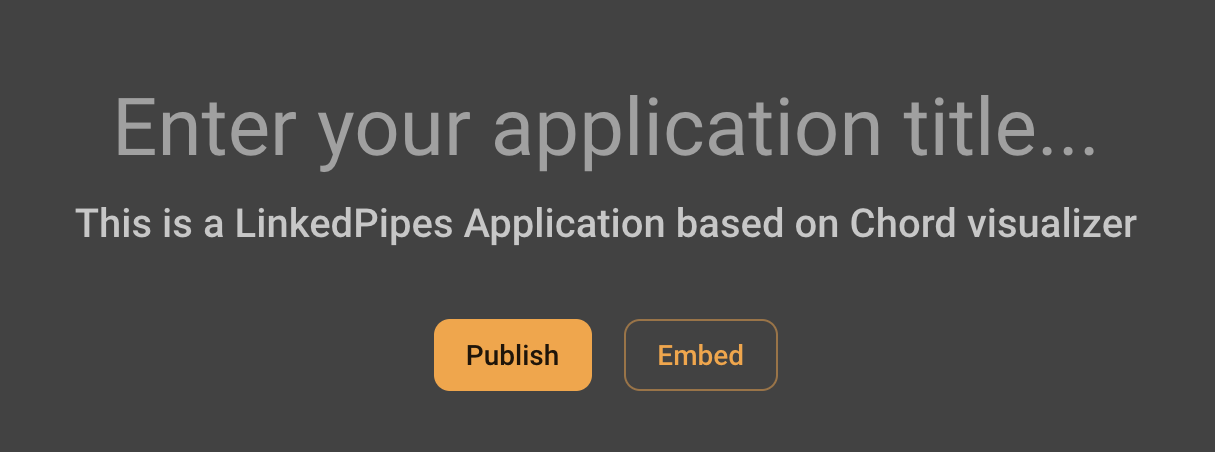
\includegraphics[width=0.8\linewidth]{lpa_create_application_page.png}}
\caption{A part of \textit{Create Application} page that invokes creation and publishing of an application.}
\label{fig:create_app_implementation_diagram}
\end{figure}

A method source code demonstrated on \autoref{lst:save_app_to_solid_chunk} is invoked by \textit{CreateVisualizerPage} and its underlying sub components. As the first step, it simply checks whether the \texttt{webId} is provided. Afterwards, the \texttt{application\-Configuration\-Object} is assembled which is a JavaScript \textit{object} with fields corresponding to \lpas{} Ontology. When passed into \textit{StorageBackend} the object is parsed into an \texttt{rdflib} graph, serialized into TTL and uploaded into \solid{} using \lpas{} package.

\begin{listing}[H]    
\begin{minted}[breaklines,frame=single,framerule=1pt,bgcolor=LightGray]{javascript}
async saveAppToSolid(
  applicationConfiguration,
  filtersConfiguration,
  webId,
  appFolder
): Promise<ApplicationMetadata> {
  if (!webId) {
    Log.error('No webID available', 'StorageToolbox');
    return;
  }

  const applicationConfigurationObject = ApplicationConfiguration.fromRawParameters(
    applicationConfiguration,
    filtersConfiguration,
    webId
  );

  return StorageBackend.uploadApplicationConfiguration(
    applicationConfigurationObject,
    appFolder,
    webId
  );
}
\end{minted}
\caption{A method from \textit{StorageToolbox} class in\lpa{} frontend, that assembles configuration object and saves it to \solid{}} 
\label{lst:save_app_to_solid_chunk}
\end{listing}

The resulting \lpa{} configuration uploaded to solid with the method from \autoref{lst:save_app_to_solid_chunk} is demonstrated on \autoref{lst:lpapp_configuration_example}. The fields with unique identifiers were replaced by sample text to improve readability of the example. 

\begin{listing}[H]    
\begin{minted}[breaklines,frame=single,framerule=1pt,bgcolor=LightGray]{turtle}
@prefix : <#>.
@prefix lp: <https://w3id.org/def/lpapps#>.
@prefix c: </profile/card#>.

<>
    a lp:VisualizerConfiguration;
    lp:applicationData "undefined";
    lp:author c:me;
    lp:backgroundColor "#106368";
    lp:configurationId "sample id";
    lp:endpoint "chord";
    lp:etlExecutionIri "sample etl iri";
    lp:filteredBy
            [
                a lp:FilterConfiguration;
                lp:enabled "true";
                lp:filterGroups [];
                lp:visible "true"
            ];
    lp:graphIri "sample graph iri";
    lp:published "2019-12-05T13:11:37.788Z";
    lp:title "My cool visualizer";
    lp:visualizerType "CHORD".
\end{minted}
\caption{An example of stored \lpa{} configuration for \textit{CHORD} visualizer in TTL} 
\label{lst:lpapp_configuration_example}
\end{listing}

As the last step of creating and publishing the \lpa{} application, the popup at \autoref{fig:lpa_published_app_popup} is presented, indicating the successful publishing of the application. 

\begin{figure}[h]
\centering
\fcolorbox{black}{white}{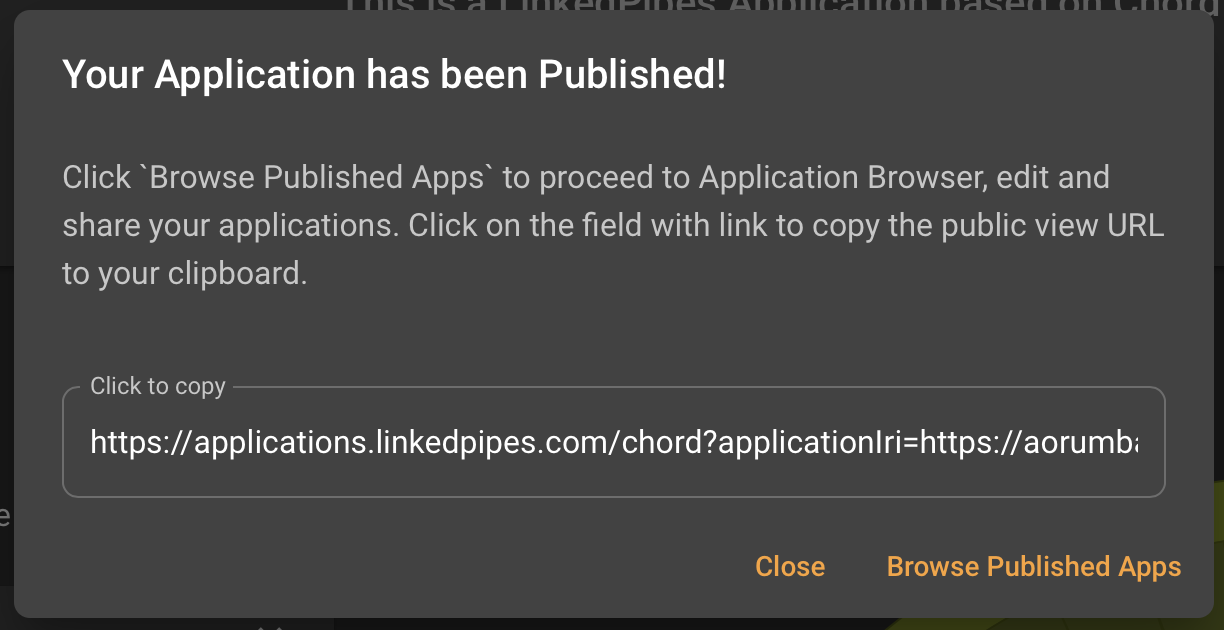
\includegraphics[width=0.8\linewidth]{lpa_published_popup.png}}
\caption{A popup presented after configuration is stored and a published url is ready to be shared.}
\label{fig:lpa_published_app_popup}
\end{figure}

This concludes the demonstration of components and functionality of both \lpa{} and \lpas{} package that implement the functional requirements on storing, publishing and creating \lpa{} configurations. 

\subsection{Configuring Application}
\label{ssssec:configuring_application_implementation}

The ability to configure the published applications had a clear and straightforward set of terms to implement. After publishing an application \lpa{} users  to \textit{rename}, \textit{delete} the configuration as well as configure and modify the filters available for the visualiser.

\subsubsection{Renaming application}

Renaming the published application is performed by executing a simple \texttt{SPARQL} query. The \textit{fetch()} method available in \textit{AuthenticationManager} abstraction from \lpas{} package is used to send the constructed request. 

\begin{listing}[H]    
\begin{minted}[breaklines,frame=single,framerule=1pt,bgcolor=LightGray]{javascript}
const sparqlQuery = `
        @prefix lpa: <https://w3id.org/def/lpapps#> .

        DELETE
        { ?configuration lpa:title ?titleValue . }
        INSERT
        { ?configuration lpa:title "${newTitle}" .}
        WHERE
        { ?configuration lpa:title ?titleValue . }
`;
\end{minted}
\caption{An example of \texttt{SPARQL} query to update the application title in configuration stored in \solid{}.} 
\label{lst:lpapp_sample_rename_app_sparql}
\end{listing}

Example on \autoref{lst:lpapp_sample_rename_app_sparql} demonstrate the \texttt{SPARQL} query used for renaming the title of \lpa{} configuration. The source code on \autoref{lst:lpapp_patch_file_with_query} demonstrate how the query is constructed and submitted to \solid{} using a class called \textit{StorageSparqlClient}.

\begin{listing}[H]    
\begin{minted}[breaklines,frame=single,framerule=1pt,bgcolor=LightGray]{javascript}
patchFileWithQuery = async (url, query) => {
  try {
    await StorageAuthenticationManager.fetch(url, {
      method: 'PATCH',
      body: query,
      headers: {
        'Content-Type': 'application/sparql-update'
      }
    });
    return true;
  } catch (error) {
    if (error instanceof Response && error.status === 404) return false;
    throw error;
  }
};
\end{minted}
\caption{The \textit{patchFileWithQuery} method in \textit{StorageSparqlClient} class is used for executing the PATCH requests to \solid{} servers.} 
\label{lst:lpapp_patch_file_with_query}
\end{listing}

\begin{figure}[h]
\centering
\fcolorbox{black}{white}{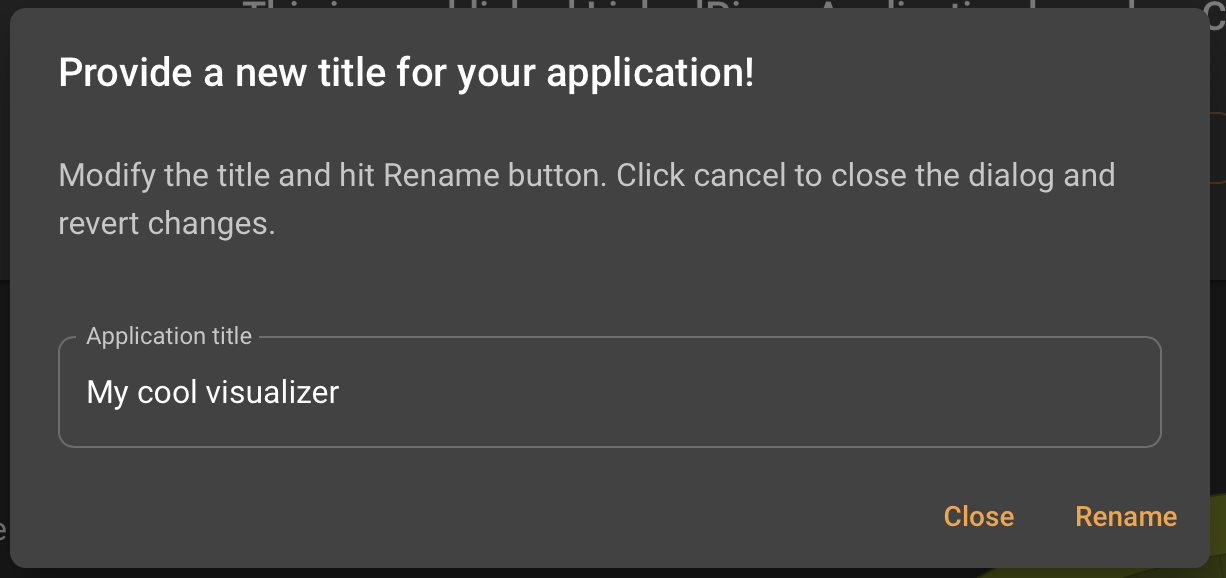
\includegraphics[width=0.8\linewidth]{lpa_rename_visualzer.png}}
\caption{A popup presented after user pressed \textit{Rename} button.}
\label{fig:lpa_rename_visualzer}
\end{figure}

On the frontend side, the rename is invoked by pressing the \textit{Rename} button from the \textit{Application Control and Setup} webpage. The user is presented with a simple popup dialog demonstrated on \autoref{fig:lpa_rename_visualzer}, where he gets an option to choose the new title of his application. This invokes the execution of the \texttt{SPARQL} query mentioned earlier.

\subsubsection{Deleting application}

Deleting an application that was previously published is a trivial task from the standpoint of \lpas{}. When user wants to delete the application he simply invokes the \textit{Delete} button either from individual application card in \textit{Storage Dashboard} webpage or inside the \textit{Application Control and Setup} webpage. Executing the deletion invokes the \textit{StorageToolbox} class that uses the \textit{deleteResource()} function from \textit{FileManager} abstraction in \lpas{} package described in \autoref{sssec:file_manager_implementation}.

\begin{figure}[hbt]
\minipage{0.3\textwidth}
  \fcolorbox{black}{white}{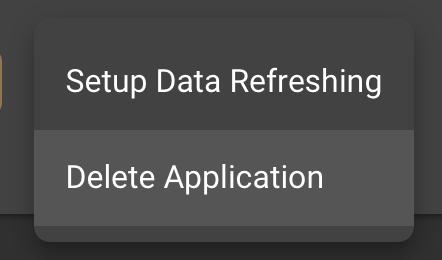
\includegraphics[width=0.8\linewidth]{lpa_delete_from_configuration_page.png}}
  \caption{Option to invoke the deletion confirmation popup on \textit{Application Control and Setup} web page}
  \label{fig:lpa_delete_from_configuration_page}
\endminipage\hfill
\minipage{0.6\textwidth}
  \fcolorbox{black}{white}{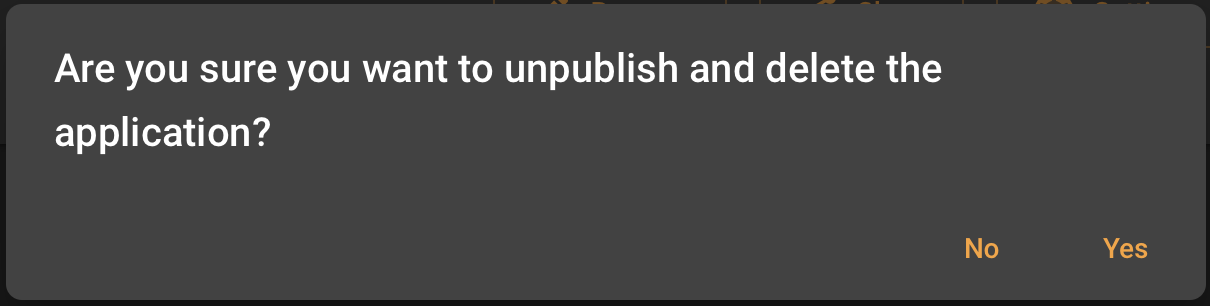
\includegraphics[width=0.8\linewidth]{lpa_delete_app_confirmation.png}}
  \caption{Popup displayed before removing published application configuration.}
  \label{fig:lpa_delete_app_confirmation}
\endminipage\hfill
\end{figure}

The popups that appear to user when he presses the \textit{Delete} button on \autoref{fig:lpa_delete_from_configuration_page} is presented on \autoref{fig:lpa_delete_app_confirmation}.

\subsubsection{Updating filters}
\label{ssssec:updating_filters_implementation}

The ability to modify the filters on a published visualizer is another important part of the \textit{Configure Application} functional requirement. The process of updating filters on published applications is invoked when a user modifies available \textit{node} or \textit{scheme} filters. For example, the UI elements on \autoref{chap:num_1} demonstrate a \textit{CHORD} visualizer containing multiple \textit{node} filters. User has an option to control \textit{state} of the filter, \textit{visibility} to the end user and \textit{interactivity} or the ability for public viewers to interact with the visualizer using the individual filters. 

\begin{figure}[h]
\centering
\fcolorbox{black}{white}{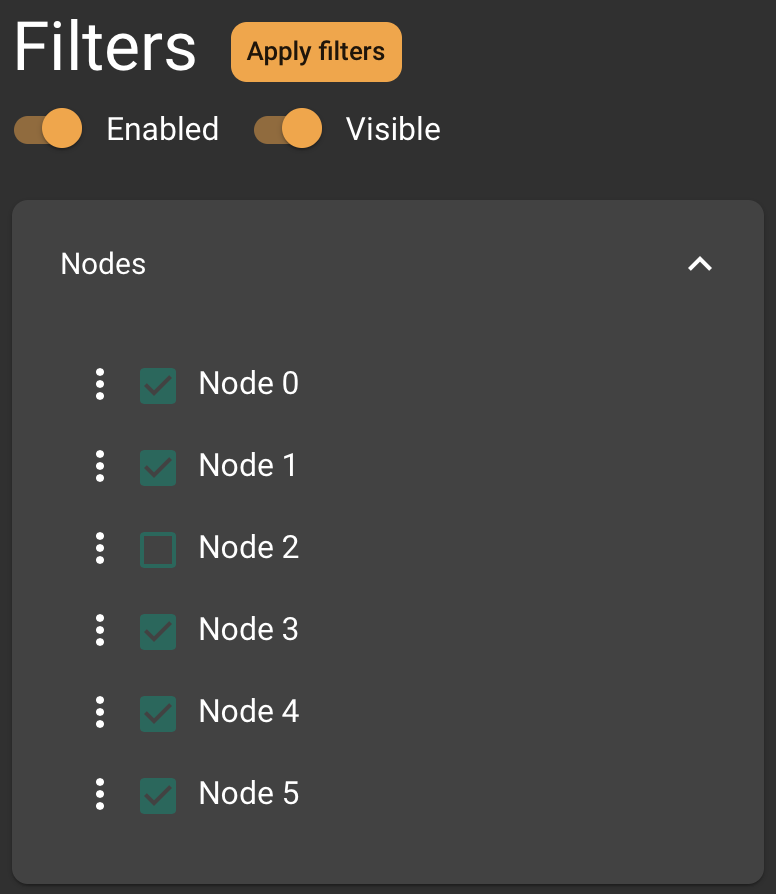
\includegraphics[width=0.5\linewidth]{lpa_filters_ui.png}}
\caption{A user interface components to interact with filters available for a visualizer.}
\label{fig:lpa_filters_interactions}
\end{figure}


The implementation of methods processing these operations are done in \textit{StorageToolbox}, \textit{StorageBackend} and \textit{StorageSparqlClient} classes, and similar to \textit{Renaming Application} procedure, the core logic simply constructs the required \texttt{SPARQL} queries and executes them using HTTP PATCH request. Example on \autoref{lst:lpapp_sample_set_filter_sparql} demonstrates the construction of \texttt{SPARQL} query that processes multiple filter selections in a single PATCH call.  

\begin{listing}[H]    
\begin{minted}[breaklines,frame=single,framerule=1pt,bgcolor=LightGray]{javascript}
let sparqlQuery = '@prefix lpa: <https://w3id.org/def/lpapps#> .';
const deleteStatements = [];
const insertStatements = [];
const whereStatements = [];

for (const node of nodes) {
  deleteStatements.push(`?selectedOption${cnt} lpa:uri "${node.uri}" .
  ?selectedOption${cnt} lpa:selected ?selected${cnt} .
  ?selectedOption${cnt} lpa:visible ?visible${cnt} .
  ?selectedOption${cnt} lpa:enabled ?enabled${cnt} .`);

  insertStatements.push(`?selectedOption${cnt} lpa:uri "${node.uri}" .
  ?selectedOption${cnt} lpa:selected "${node.selected}" .
  ?selectedOption${cnt} lpa:visible "${node.visible}" .
  ?selectedOption${cnt} lpa:enabled "${node.enabled}" .`);

  whereStatements.push(`?selectedOption${cnt} lpa:uri "${node.uri}" .
  ?selectedOption${cnt} lpa:selected ?selected${cnt} .
  ?selectedOption${cnt} lpa:visible ?visible${cnt} .
  ?selectedOption${cnt} lpa:enabled ?enabled${cnt} . `);
}

sparqlQuery += `
  DELETE { ${deleteStatements.join('\n')} }
  INSERT { ${insertStatements.join('\n')} }
  WHERE { ${whereStatements.join('\n')} }
`;
\end{minted}
\caption{An example of \texttt{SPARQL} query to update the state of multiple \textit{node} filters selected by user.} 
\label{lst:lpapp_sample_set_filter_sparql}
\end{listing}

One of the additional features implemented within the bounds of that requirement is the ability to reflect the applied changes in any field of the application configuration RDF file using socket listeners. In other words, if a user is editing filters on his visualizer and some other user is looking at his visualizer on some webpage where it is published, he will see the changes being applied in real-time. This is implemented using the \texttt{rdflib.js} library that is accessed via \lpas{} package. The \autoref{lst:lpap_add_listeners_function} demonstrates a simple utility function available at \textit{StorageBackend} and it is invoked when application configuration is being fetched for the first time. 


\begin{listing}[H]    
\begin{minted}[breaklines,frame=single,framerule=1pt,bgcolor=LightGray]{javascript}
registerChanges(url: string, callbackOnRefresh: Function = undefined) {
  if (this.alreadyAddedDownstreamListeners.indexOf(url) === -1) {
    const doc = $rdf.sym(url).doc();
    this.updater.addDownstreamChangeListener(doc, callbackOnRefresh);
    this.alreadyAddedDownstreamListeners.push(url);
  }
}
\end{minted}
\caption{Implementation of helper utility that uses feature of \texttt{rdflib} to invoke any callback when a change in a specified RDF resource is detected.} 
\label{lst:lpap_add_listeners_function}
\end{listing}

\subsection{Storage Management}

The Storage Management functional requirement defines an implementation request to have an ability to \textit{move}, \textit{rename} or \textit{copy} the root folder with all configurations inside the storage. From the perspective of \lpas{} it implies controlling the root LDP Basic Container that stores all configurations.

\begin{figure}[h]
\centering
\fcolorbox{black}{white}{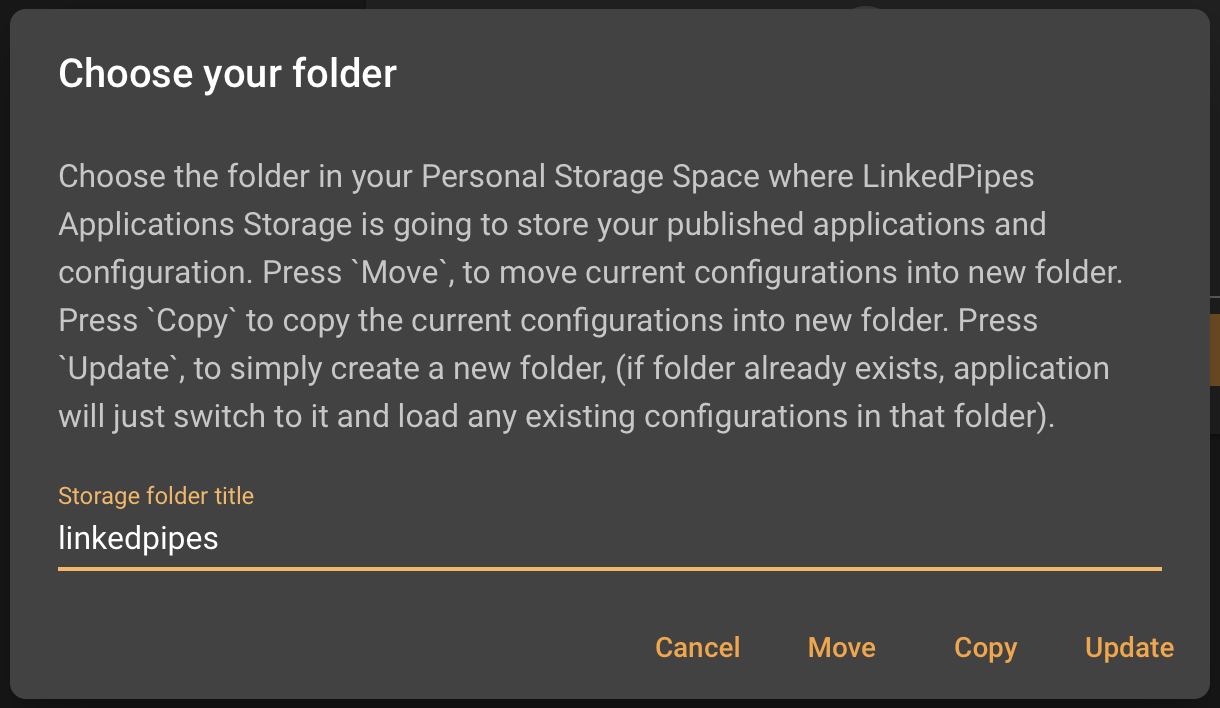
\includegraphics[width=0.7\linewidth]{lpa_updating_root_folder.png}}
\caption{A final render of Storage Control Panel component.}
\label{fig:lpa_updating_root_folder}
\end{figure}

Since the description in \autoref{sssec:storage_control_panel_implementation} already provided all details on implementing this requirement, this section will demonstrate the final renders of implemented components to perform the operations stated in the requirement. The user interface demonstrated on \autoref{fig:lpa_updating_root_folder}, performs the functionality as requested in the definition of the requirement. It is invoked via \textit{Settings} webpage under \textit{Application Storage} tab when user clicks on \textit{Change folder} tab. 

\subsection{Visualizer Access Control}

The Visualizer, Access Control requirement, defines how the creator of an application can control public access to visualizer or share it with only a specified set of contacts. From the \lpas{} standpoint, this implies controlling the ACL files of individual \lpa{} configurations expressed in RDF.

\begin{figure}[h]
\centering
\fcolorbox{black}{white}{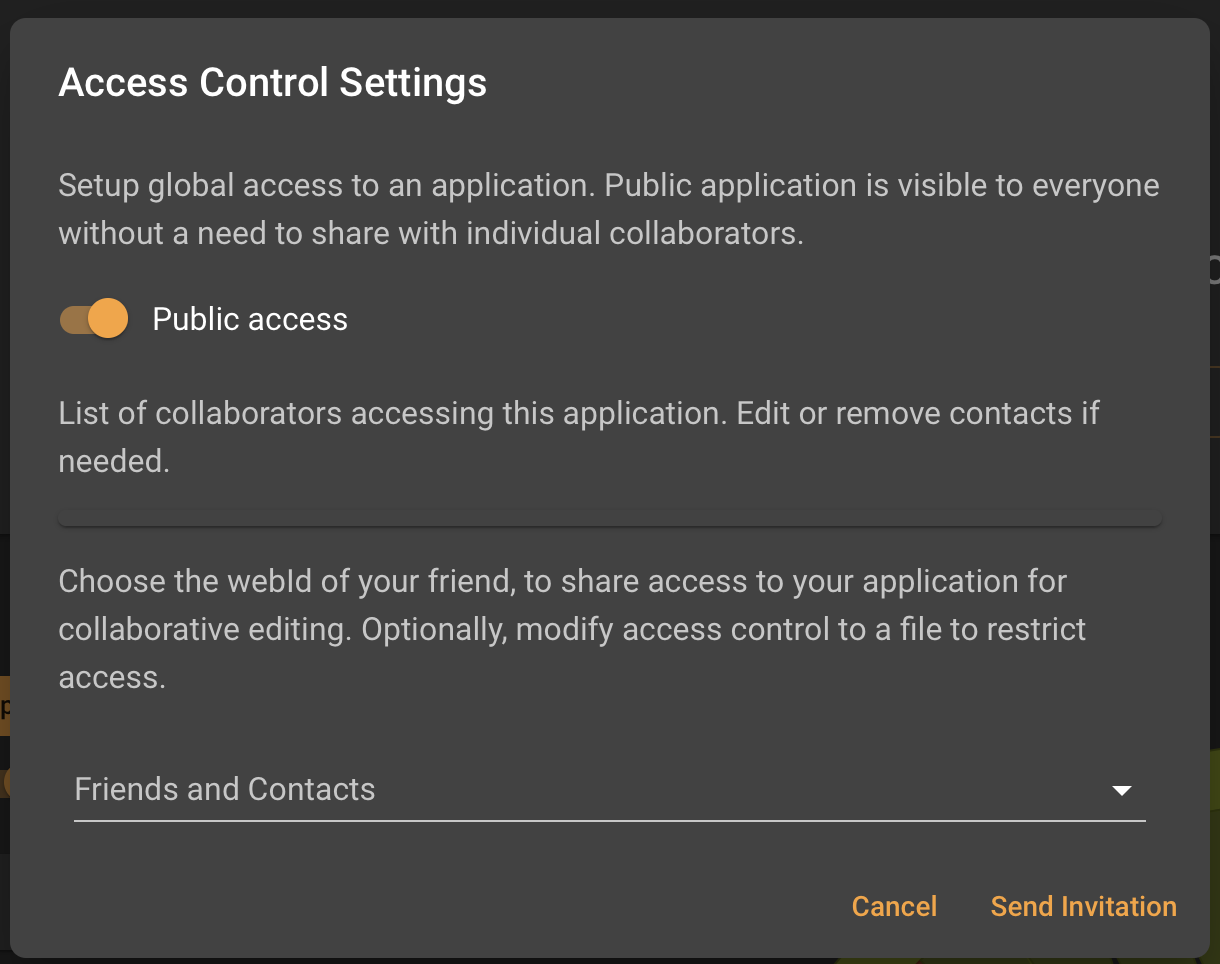
\includegraphics[width=0.7\linewidth]{lpa_access_control_setup.png}}
\caption{Access control configuration popup for published application.}
\label{fig:lpa_access_control_setup}
\end{figure}

The implementation of \textit{AccessControlManager} abstraction in \autoref{sssec:access_control_manager_implementation} is the essential building block that was used to implement a set of React Components to allow modifying access control privileges of published visualizers. The \autoref{fig:lpa_access_control_setup} demonstrate an final render of a React Component that is presented to user when he clicks on \texttt{Access Control} drop down item on \textit{Application Control and Setup} webpage. The component is implemented in \textit{StorageAccessControlDialog} file which is a simple stateful React Component. The main elements of that popup can be described as follows:
\begin{itemize}
    \item \textit{Public access} switch, this element controls the default public access to a published application. By default, \lpa{} sets the \textit{READ} public access so that anyone can access the published application by default. However, the user has an option to toggle the control element and disable default public visibility. 
    \item \textit{List of collaborators}, this element lists the contacts knows to user's \textit{WebID}. The querying of knows contacts is performed using \texttt{rdflib} library accessed via \lpas{} package. 
    \item \textit{Friends and Contacts} dropdown, this element is a selector for sending invitations to share the published visualizer with other users of the platform. The next subsection will provide more details on the collaborative sharing feature implemented as an additional functionality on top of the initial functional requirement. Collaborative sharing features implementation is inspired by \textit{\gls{LDN}} \cite{ldn} and uses the \textit{ActivityStreams} vocabulary \cite{activitystreams}. However, due to the specificity of \lpa{}, it does not strictly follow all requirements of that specification. 
\end{itemize}

\subsubsection{Collaborative sharing}
\label{ssssec:collaborative_sharing}

Collaborative sharing allows users of \lpa{} platform to share their visualizers with other users of the platform. The sharing process implementation is inspired by Linked Data Notifications specification and involves the generation of an invitation file that send to the recipients inbox. The \autoref{fig:lpas_sharing_application} demonstrates the process of submitting an invitation in detail.

\begin{figure}[h]
\centering
\fcolorbox{black}{white}{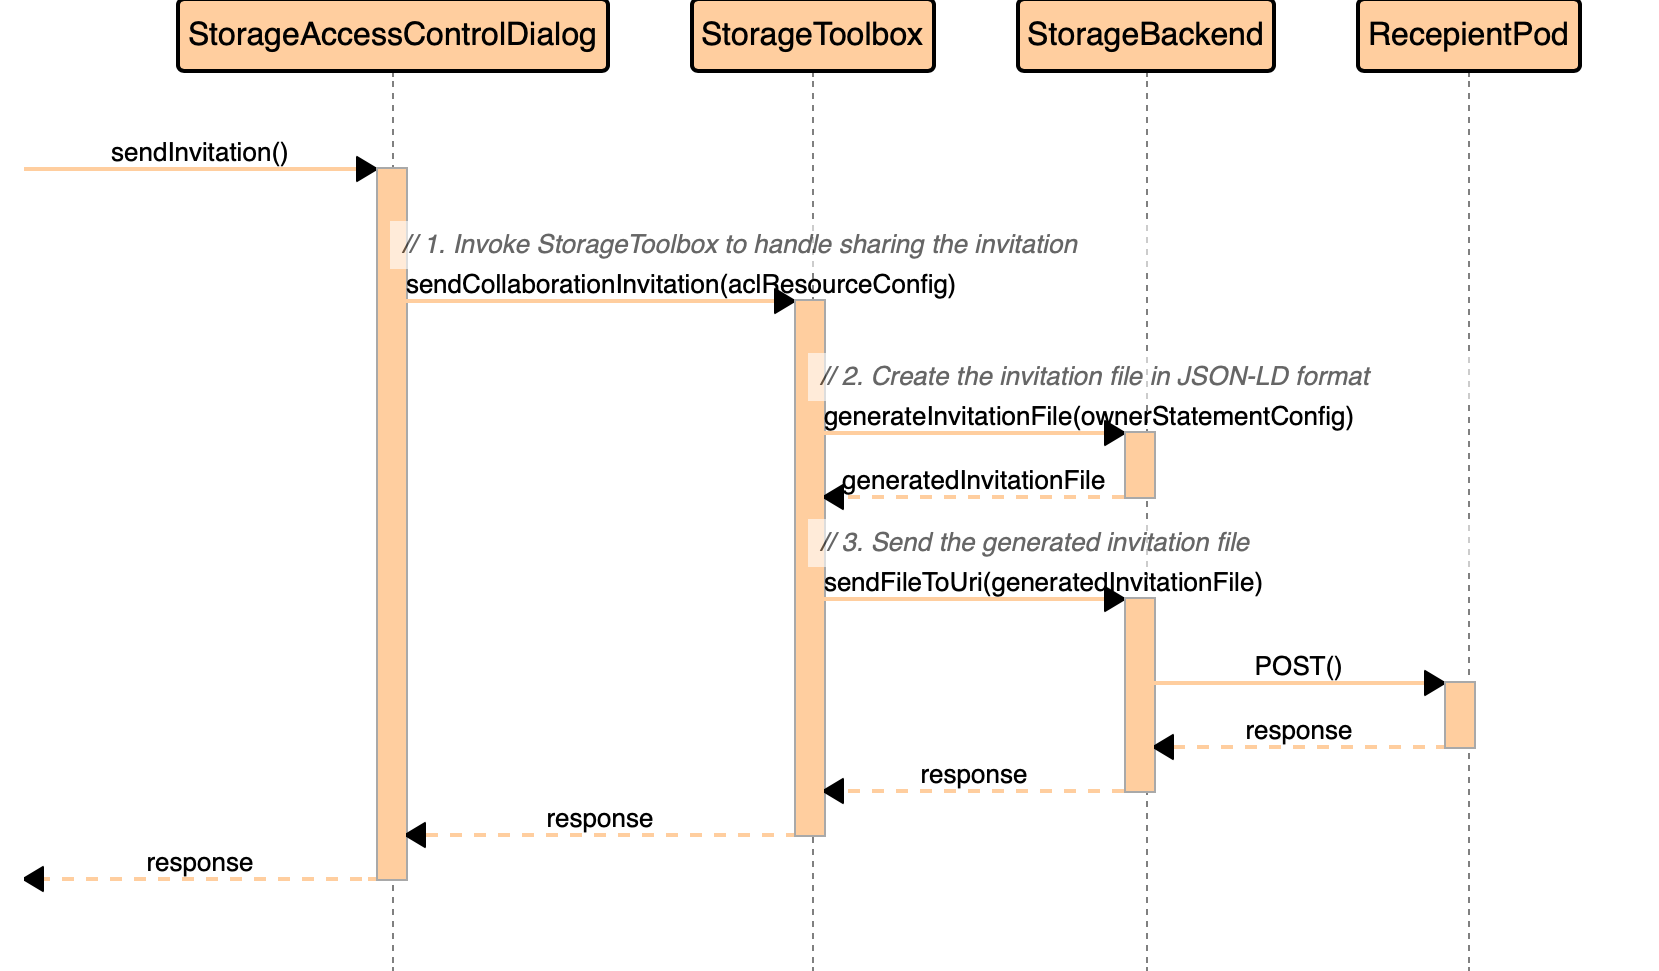
\includegraphics[width=0.8\linewidth]{lpas_sharing_application.png}}
\caption{A sequence diagram of implemented sharing functionality for collaborative editing.}
\label{fig:lpas_sharing_application}
\end{figure}
  
The steps can be described as follows:
\begin{enumerate}
    \item Firstly, the \textit{sendInvitation()} function is invoked from \textit{StorageAccessControlDialog} React Component, specifically when users chooses his available list of contacts and presses submit invitation button.
    \item As a next step, \textit{StorageToolbox} redirects the request to lower-level \textit{StorageBackend} class.
    \item The \textit{StorageBackend} class generates the invitation RDF in JSON-LD format using \texttt{rdflib} library from \lpas{} package.
    \item The \textit{StorageBackend} class sends the invitation file to recepients inbox folder using \textit{FileManager} abstraction from \lpas{} package. The exact inbox path is known by parsing the recipient's profile card associated with his WebID.
    \item Asyncronous response is returned of the operations is propagated back to \textit{StorageAccessControlDialog} for further processing. 
\end{enumerate}
 
\begin{figure}[h]
\centering
\fcolorbox{black}{white}{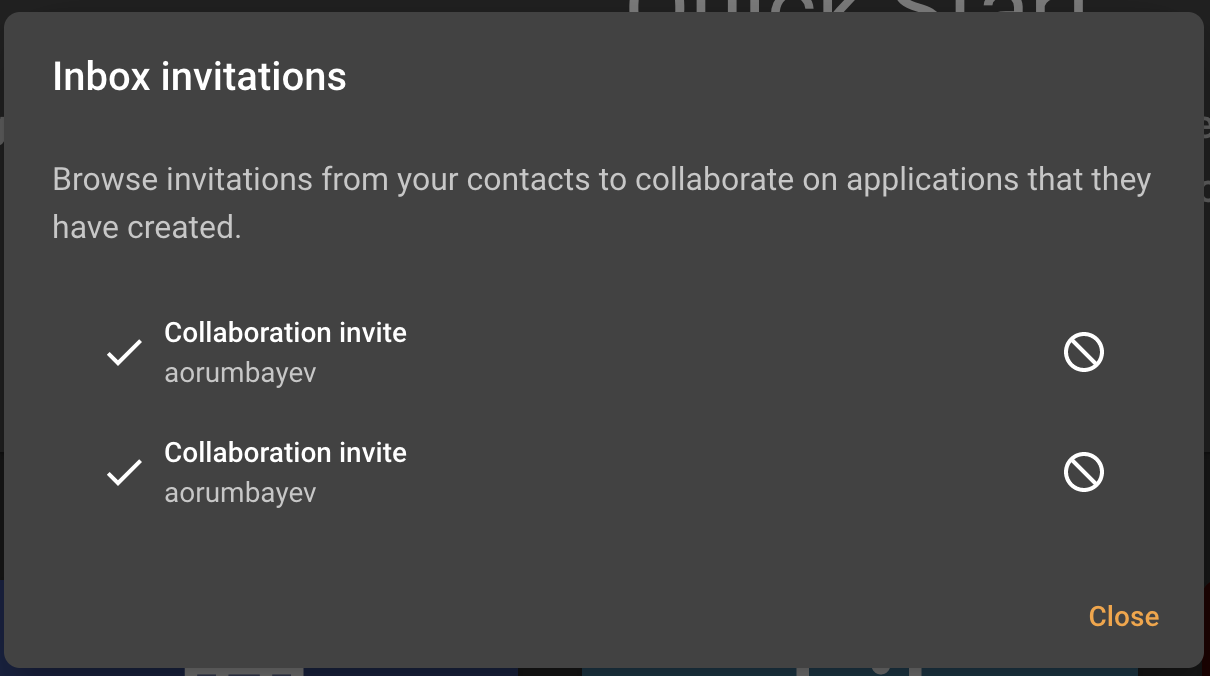
\includegraphics[width=0.7\linewidth]{lpa_inbox_with_invitations.png}}
\caption{An inbox dialog popup with two new invitations to collaborate on application.}
\label{fig:lpa_inbox_with_invitations}
\end{figure}
  
 
It is important to note that the recipient is assumed to be a user of \lpa{} platform. Once invitation is send, whenever recipient opens the platform, the listener inside \textit{AppRouter} class will check the inbox for new invitations and display new invitations in inbox popup demonstrated on \autoref{fig:lpa_inbox_with_invitations}. If user \textit{Accepts} the invitation, the invitation JSON-LD file is transformed into a shared configuration file by extracting URI to an application and placing it under a folder named \textit{sharedApplications} in the root storage folder and a response notification is sent back to the sender. Once sender receives the \textit{Accept} notification, it sets the \textit{READ} and \textit{WRITE} access to the application configuration for the recipient. If user \textit{Declines} the invitation, the invitation is deleted from the inbox without any further processing.

\begin{figure}[h]
\centering
\fcolorbox{black}{white}{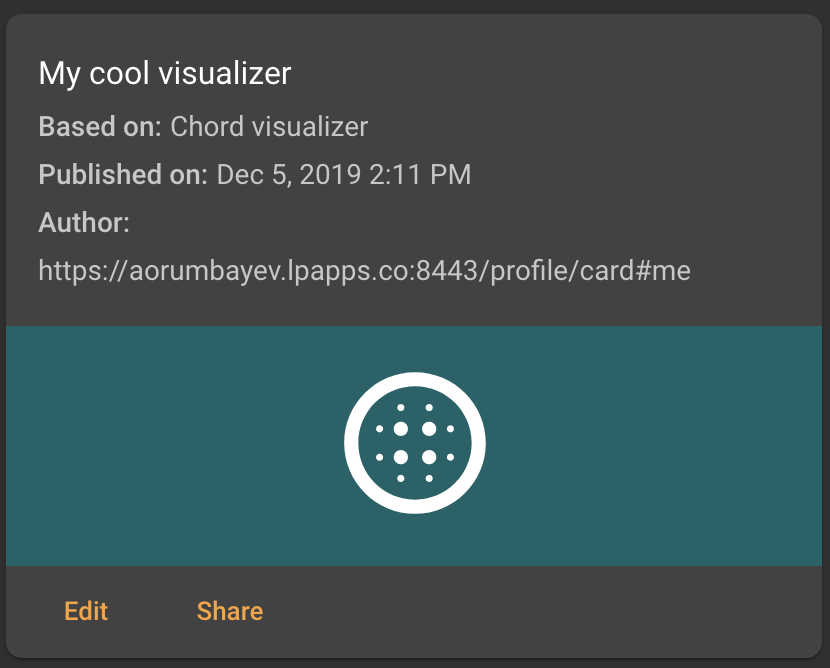
\includegraphics[width=0.7\linewidth]{lpa_shared_visualizer_card.png}}
\caption{A shared visualizer card displayed to recipient in his Storage Dashboard after he accepts the invitation.}
\label{fig:lpa_shared_visualizer_card}
\end{figure}

The \autoref{chap:num_1} demonstrates the shared application appearing in the shared applications storage dashboard of the recipient. In addition to that, the code on \autoref{lst:lpa_example_invitation_json_ld} demonstrates the example of the generated invitation being send to recipient in JSON-LD format using \textit{ActivityStreams} vocabulary. 

\begin{listing}[H]    
\begin{minted}[breaklines,frame=single,framerule=1pt,bgcolor=LightGray]{json}
{
  "@context": "https://www.w3.org/ns/activitystreams",
  "type": "Invite",
  "actor": "https://sender.lpapps.co:8443/profile/card#me",
  "name": "lpapps_invite",
  "object": {
    "type": "Link",
    "href": "https://sender.lpapps.co:8443/
    linkedpipes/configurations/1575551497789.473.ttl"
  },
  "published": "2019-12-06T20:04:02Z",
  "target": "https://recipient.lpapps.co:8443/profile/card#me"
}
\end{minted}
\caption{An example invitation to collaborate on a published application.} 
\label{lst:lpa_example_invitation_json_ld}
\end{listing}

The collaborative aspect is basic and only allows the recipient to rename the title of the application and modify and persist the selection of available filters. The changes are reflected in real-time using socket connection to \solid{} server as initially described in \autoref{ssssec:updating_filters_implementation}.

To sum up, the following section iterated over each functional requirement stated by \lpa{} and demonstrated the detailed description of implementation to comply with those requirements. The section also continued the storage-related React Components implementation details provided in \autoref{sssec:lpas_storage_frontend_implementation} and demonstrated finalized renders of those components that closely follow the initial mocks designed in \autoref{chap:num_4}. 

\section{Implemented non-functional requirements}
\label{ssec:non_functional_requirements_implementation}

The section provides a general overview of implementation of non-functional requirements stated in \autoref{ssec:non_functional_requirements}. Due to the majority of requirements being covered simply by the core functionality of the \solid{} project itself, the implementation details of individual requirements are less descriptive than descriptions in \autoref{ssec:overview_of_implemented_requirements}. It is also important to note that this section provides the implementation overview of all stated functional requirements defined in \autoref{ssec:non_functional_requirements}.

\subsection{Compatibility with latest tools}

The implemented solution consists of three parts:
\begin{itemize}
    \item The \lpas{} package, an npm package containing the generic abstractions performing low-level interactions with instances of \solid{} servers. Relies on \texttt{rdflib}, \texttt{solid-auth-client} and \texttt{solid-auth-cli} libraries. All third party packages are pinned, stable and indirectly unit tested, more details on testing is provided in \autoref{chap:num_7}. 
    \item The Storage React components, a set of frontend components written in ES6 inside the \lpa{} package. No additional third party packages are introduces to \lpa{} with these components, except for \lpas{} package. 
    \item The \lpas{} ontology, a vocabulary designed with \texttt{Protégé} and published with \texttt{Ontoology}. Used in \lpa{} by accessing its public hosted instance, therefore no additional third party packages are introduced.
\end{itemize}

\subsection{Clean APIs and libraries}

The whole intent of creating the \lpas{} package was to refactor and redesign the abstractions interacting with solid inside \lpa{} frontend codebase. Therefore, the final refactored implementation is easier to maintain and use by LPA developers due to usage of TypeScript, extensive automated testing coverage covered in \autoref{chap:num_7}, and documentation included in \autoref{chap:num_8}.

\subsection{Continuous Integration and Delivery}

The \lpas{} package is located in a separate GitHub repository, has an automated continuous delivery pipeline invoking unit test, code formatting, and linting. The continuous delivery aspect publishes new npm versions in is semi-automated manner. The frontend storage components in \lpa{} are incorporated into frontend codebase. Hence they are validated using the \lpa{} CI and CD pipelines. Some improvements into \lpa{} testing pipelines were introduced, and they are described in detail in \autoref{chap:num_7}.

\subsection{Easy integration with \lpa{}}

The \lpas{} package is distributed via npm, and seamlessly integrated into \lpa{} using the package management software. The frontend storage components are implemented inside the frontend codebase. However, they also maintain a consisted structure that improves code readability and defines the logical separation between functionalities of \lpa{} and \lpas{}.

\subsection{Decentralized storage}

The solution for this non-functional requirement is covered by \solid{} specification. Since \solid{} servers are decentralized by design, it means that the \textit{AuthenticationManager} from \lpas{} package allows the users of \lpa{} to authenticate with any arbitrary instance of their private \solid{} server instances or instances from third-party \solid{} providers. The \textit{FileManager} abstraction also allows users to move the created \lpa{} configurations between \solid{} PODs within a \solid{} server instance or between different instances of compatible \solid{} servers.
\chapter{Evaluation}
\label{chap:num_6}

This chapter briefly describes and evaluates the results, recognition, and notable achievements obtained after evaluating final \lpas{} solution inside the production instance of \lpa{} platform \footnote{\url{https://applications.linkedpipes.com}}.

\section{Benefits of \solid{}}

Usage of \solid{} technology significantly enhanced the initial functionality of \lpa{}, allowing to utilize the full benefits of Semantic Web and Linked Data management. The section describes the individual advantages and their influence on the improvement of \lpa{} platform.

\subsection{ACL managed applications}

Access Control Management is one of the core features provided by \solid{}. The implementation and integration of \textit{AccessControManager} abstraction from \lpas{} package, ability for \lpa{} developers to easily create, and edit the ACL files. From the perspective of \lpa{} platform users, this provided the ability to have full control and management over the data created by the \lpa{} but stored in \lpas{} package. 

\subsection{Everything is an RDF resource}

Storing \lpa{} applications in \solid{} means storing their configuration files expressed in TTL RDF format. Therefore, adding more value to the date as it can be queried, filtered, or transformed in any way possible using SPARQL querying language. Consider a use case where an experienced data journalist and developer who created and owns a set of multiple visualizers displaying markers on a map, he recently discovered a new dataset that consists of smaller datasets for applications he created previously. He can use SPARQL to analyze his configurations stored in his \solid{} POD and create a new configuration by aggregating the filters from smaller application configurations and \lpa{} platform will attempt to re-create the application for a new configuration.
Storing data as RDF also provides possibilities for future enhancements of \lpas{}. For instance, consider a case when several \lpa{} applications are embedded in a service similar to Wikipedia. One could easily create a SPARQL query to extract URIs to those visualizations and query any of the components of that configuration. 

\subsection{Provider agnostic storage}

By design, \solid{} servers are decentralized, a single \solid{} POD can host multiple \solid{} POD, and user own the data inside each of the PODs. When an \lpa{} platform users creates his first WebID and a \solid{} POD, all of \lpa{} configurations are created inside the \solid{} POD in authenticated \solid{} server. However, it is not bound to any specific implementation of \solid{} servers, it is completely agnostic and supports any implementation of a server that complies to \solid{} specification. In addition to that, user has an ability to use the \textit{Storage Control Panel} to move the created configurations within their PODs. The \solid{} POD webpage also allows users to move any data between different instances of \solid{} servers.

\section{Results and achievements}

The sections provide a brief overview of notable achievements and recognitions of \lpa{} platform that was directly and indirectly influenced by usage of \solid{} technology. 

\subsection{Recognition on official \solid{} website}
\label{sssec:recogniition_on_solid}

In July 2019, after the first production release of \lpa{} platform with a partial implementation of \lpas{}, the project was approved and added into the official list of \solid{} applications on the repository of \solid{} organization in GitHub. The screenshot of \autoref{fig:lpa_listing_on_solid} demonstrates the listing of the project on the official website.

\begin{figure}[h]
\centering
\fcolorbox{black}{white}{\includegraphics[width=0.7\linewidth]{lpa_listing_on_solid.png}}
\caption{Listing of \lpa{} platform on official \solid{} project website.}
\label{fig:lpa_listing_on_solid}
\end{figure}

\subsection{Comments from Sir Tim Berners-Lee}
\label{sssec:comments_from_tim}

During the whole development lifecycle of the \lpas{} project, active communication with the community helped to clarify many intricated nuances in the rapidly changing development ecosystem of \solid{} project. The creator of the \solid{} project is an active participant on \textit{Gitter} \footnote{\url{https://gitter.im}} channels related to the project. During the implementation of \textit{FileManager} abstraction, multiple questions asked on \solid{} channels on Gitter were answered by Sir Tim Berners-Lee, providing useful insights and motivation to contribute into the development of \solid{} as a web standard for decoupling and decentralizing the web. One of several interactions is demonstrated on a screenshot of a conversation of \autoref{fig:comments_from_tim_bl}.

\begin{figure}[h]
\centering
\fcolorbox{black}{white}{\includegraphics[width=0.7\linewidth]{comments_from_tim_bl.png}}
\caption{One of multiple interactions with creator of \solid{} on \solid{} community chat.}
\label{fig:comments_from_tim_bl}
\end{figure}

\subsection{User traction on \lpa{} platform}
\label{sssec:user_traction_of_platform}

Evaluation of final release of \lpa{} platform with finalized \lpas{} solution received a feedback from multiple \solid{} community members. Additionally one of the members of \gls{BARTOC} organization evaluated the application, provided a positive feedback and published an application stored in \solid{} using \lpas{} on official website of organization \footnote{\url{https://new.bartoc.org/node/332}}. \TODO{This is nice, however, it says that the app was deleted - therefore either fix this if possible, or consider commenting on this.}

\begin{figure}[hbt]
\minipage{0.4\textwidth}
  \fcolorbox{black}{white}{\includegraphics[width=0.8\linewidth]{google_analytics_users.png}}
  \caption{Google Analytics traction of users of test \lpa{} platform instance over a period of six months.}
  \label{fig:google_analytics_users}
\endminipage\hfill
\minipage{0.6\textwidth}
  \fcolorbox{black}{white}{\includegraphics[width=0.8\linewidth]{community_post_users.png}}
  \caption{Feedback, views and comments on for \lpa{} launch on official \solid{} community forum.}
  \label{fig:community_post_users}
\endminipage\hfill
\end{figure}

Additionally, screenshots on \autoref{fig:google_analytics_users} and \autoref{fig:community_post_users} demonstrate the traction of \solid{} community users. Release of the \lpa{} platform with \lpas{} storage was posted on official \solid{} community forum, where a notable positive commentary was left by one of the founders of \textit{Virtuoso Universal Server} Kingsley Uyi Idehen \footnote{\url{http://dbpedia.org/page/Kingsley_Uyi_Idehen}}. Over the period of six month starting July and ending on December 2019, over 300 users interacted with test instance of \lpa{} as demonstrated on \autoref{fig:google_analytics_users}.
\chapter{Testing}
\label{chap:num_7}

The following section will provide an overview of testing practices followed during the implementation described in \autoref{chap:num_5}. The chapter will start by describing the preliminary technologies used for implementing automated testing, integration, and delivery pipelines as well as libraries used for unit testing of TypeScript base \lpas{} package.

\section{Technologies used}

The main development stack consisted of the following technologies: 
\begin{itemize}
    \item \textit{\texttt{ava.js}} \footnote{\url{https://github.com/avajs/ava}} is a Node.js unit testing library. It provides a clean and minimalistic syntax for writing tests, concurrent tests execution, includes TypeScript definitions and supports asyncronous functions. All of the aforementioned factors were considered when choosing this package as main unit testing library for \lpas{} package.
    
    \item \textit{\texttt{tslint}} \footnote{\url{https://palantir.github.io/tslint/}} is an extensible static analysis tool that checks TypeScript code for readability, maintainability, and functionality errors. It is widely supported across modern editors and build systems and can be customized with your own lint rules, configurations, and formatters.
    
    \item \textit{\texttt{istanbul.js}} \footnote{\url{https://istanbul.js.org/}} is a code coverage analyzer. It checks ES2015+ JavaScript code with line counters providing a very extensive overview of all classes and their coverage.
    
    \item \textit{Travis CI} \footnote{\url{https://travis-ci.org/}} is a hosted, distributed continuous integration service used to build and test software projects hosted at GitHub. Travis CI is used to check that newly committed code does not break the build and, consequently, the system. This ensures that developers are not disrupted and that the system remains stable. It is also able to run available automated tests to check further that the system is working correctly, even if the build isn't broken.

    \item \textit{Renovate} \footnote{\url{https://docs.renovatebot.com/}} is an automated dependency updater. Multi-platform and multi-language. Due to various dependencies used in the \emph{frontend} web component, it is crucial to keep the project up to date with the latest stable software releases. Renovate is set up and being triggered using Github Webhooks each weekend to check for updates in \texttt{package.json} and make a pull request to \texttt{master} and \texttt{develop} branches if any available.

    \item \textit{Codecov} \footnote{\url{https://codecov.io/}} is an automated code review tool that allows developers to improve code quality and monitor technical debt. Codecov automates code reviews and monitors code quality on every commit and pull request. It reports back the impact of every commit or pull request in new issues concerning code style, best practices, security, and many others. It monitors changes in code coverage, code duplication, and code complexity. It allows developers to save time in code reviews, tackle issues efficiently, and overall makes the system maintainability much easier.
    
    \item \textit{Slack} \footnote{\url{https://slack.com/}} a cloud-based proprietary instant messaging platform developed by Slack Technologies. The platform was used for automated notifications from GitHub and Travis-CI to report the states of executed CI and CD pipelines and for communication with the \lpa{} developers.
\end{itemize} 

\section{Unit testing}
\label{ssec:lpas_unit_testing}

Every class in \lpas{} package was unit tested using the ava.js library. The convention used required in-place creation of a file with ava.js tests definitions named identical to a TS file to be tested but with \texttt{.spec.} prefix appended before the file extension. The code on \autoref{lst:unit_testing_create_resource} demonstrates the example serial ava.js test executed in order. The asynchronous \textit{createResource} can be reused in multiple ava.js tests improving code reusability while writing new tests.

\begin{listing}[H]    
\begin{minted}[breaklines,frame=single,framerule=1pt]{javascript}
async function createResource(t: any, input: any, expected: any): Promise<any> {
  const result = await StorageFileManager.createResource(input);
  logger.info(result.text());
  t.is(result.status, expected);
}

test.serial(
  'createFolderResource',
  createResource,
  folderConfigurationResource,
  201
);
\end{minted}
\caption{An example of a reusable asynchronous test chunk and single serial ava.js test for \textit{createResource()} method from \textit{FileManager} abstraction in \lpas{} package.} 
\label{lst:unit_testing_create_resource}
\end{listing}

The istanbul.js JavaScript coverage library has integration with ava.js. The official command-line interface of istanbul.js, called \texttt{nyc} is used to invoke the unit tests to both run the tests and visualize the test results in the terminal in a convenient format.

Unit tests are automatically executed on every push to any remote branch on \lpas{} package repository. More details on executing the unit tests in automated pipelines are provided in next section.

\section{Continious Integration and Delivery}
\label{ssec:integration_and_delivery}

The section will provide details on implementing automated integration and delivery pipelines using Travis CI.
The terms Continuous Integration stands for a development practice that requires a developer to integrate his latest commits to a shared repository regularly. On the other hand, the name Continuous Delivery stands for an ability to deliver code changes of any type to production in a quick, safe, and automated way. Both of the practices were taken into consideration while implementing the \lpas{} package. 

\subsection{Using Travis CI}
\label{ssec:travis_ci_lpa}

Travis CI was used in pairs with the GitHub platform. As the first step, the service was connected with \lpas{} package GitHub repository using Webhooks \footnote{\url{https://en.wikipedia.org/wiki/Webhook}}. Secondly, a special YAML configuration file was added to all branches of \lpas{} repository. The configuration file defined the integration and delivery pipelines to be executed inside Travis CI. Using a special feature called \textit{build matrix}, the \lpas{} was set to be unit tested automatically in concurrent manner on both Node.js \texttt{v10.x} and Node.js \texttt{v12.x}. 

The branch protection rules were also applied to \texttt{dev} and \texttt{master} branches on \lpas{} repository. The additional step in Travis CI pipeline configuration was added for \texttt{master} branch. Every push on remote \texttt{master} on \lpas{} repository also involves deployment to npm. Failed build states are propagated into a special slack channel in \lpa{} Slack workspace, channel is dedicated specifically for reporting CI and CD pipeline execution statuses for all branches on \lpas{} repo.

\subsection{Integration testing in \lpa{}}

The diagram on \autoref{fig:lpas_ci_integration} is a detail demonstration of how \lpa{} and \lpa{} package are integration tested in automated and semi-automated manner. It is important to note that the example on diagram considers a case when \lpas{} developer merges changes into \texttt{master} branch of \lpas{} package.

\begin{figure}[h]
\centering
\fcolorbox{black}{white}{\includegraphics[width=0.8\linewidth]{lpas_ci_integration.png}}
\caption{A detailed overview of CI and CD pipeline interaction for \lpa{} and \lpas{}.}
\label{fig:lpas_ci_integration}
\end{figure}

The operational flow can be described as follows:
\begin{enumerate}
    \item \textit{\lpas{} developer pushes code to \texttt{master} branch}, the code is pushed to a remote GitHub repository. This triggers the Travis CI and Codecov reviews via Webhooks.
    \item \textit{Travis CI evaluates the results of pipeline}. If result is successfull it automaticall pushes the new version into npm and updates the static documentation for TypeScript classes. If failed, then the \lpas{} developer is notified on Slack channel with a report on why the pipeline is failed.
    \item \textit{Renovate bot polls for new \lpas{} releases}, the Renovate bot instance attached to \lpa{} platform repository periodaclly polls npm and opens a Pull Request with new \lpas{} package to \lpa{} platform on a branch called \texttt{dependency-updates}. 
    \item \textit{The \lpa{} developer is notified via Slack}. When a Pull Request into \lpa{} codebase is opened by Renovate, it notifies the \lpa{} developer via Slack to review the Pull Request and merge new release of \lpas{} package.
\end{enumerate} 
\chapter{Documentation}
\label{chap:num_8}

The following chapter provides the information on available documentation resources implemented for both \lpas{} package and \lpa{} Storage Components. Selected code snippets demonstrate the core usage and provide detailed references for hosted documentations. The first section will give the developer guide to the documentation of \lpa{} package hosted on GitHub Pages. The second section will provide an overview of how \lpa{} Storage Components were integrated into documentation resources of \lpa{} platform.

\section{\texttt{npm} package}

The package is source codes are available at public GitHub repository \footnote{\url{https://github.com/aorumbayev/linkedpipes-storage}} and corresponding page on npm \footnote{\url{https://www.npmjs.com/package/linkedpipes-storage}}. The generic documentation on repository \textit{README}, as well as on a webpage at npm, includes the installation guide and a quick start on creating, editing, and deleting resources using a folder as an example. 

More detailed and developer oriented documentation is available on repository GitHub Page \footnote{\url{https://aorumbayev.github.io/linkedpipes-storage}}. The website is generated and published as a part of automated CI and CD pipeline demonstrated at \autoref{fig:lpas_ci_integration}. The documentation is generated using \texttt{typedoc} \footnote{\url{https://github.com/TypeStrong/typedoc}}, a documentation generator for TypeScript project. The codebase is annotated using \texttt{tsdoc} \footnote{\url{https://github.com/microsoft/tsdoc}}, an official TypeScript comment standard developed by Microsoft.

The typedoc documentation provides the overview of entire \lpas{} project codebase in the following order:
\begin{enumerate}
    \item \textit{Enumerations} description of all enumeration types in codebase.
    \item \textit{Classes} description of all class types in codebase.
    \item \textit{Interfaces} description of all interface types in codebase.
    \item \textit{Variables} description of all variable types in codebase.
    \item \textit{Functions} description of all function types in codebase.
\end{enumerate}

Every individual type is expanded into a detailed description of its sub-elements. For instance, every class type documentation is structured as follows:
\begin{enumerate}
    \item \textit{Constructors} description of all class constructors, input parameters and return values.
    \item \textit{Properties} description of all properties of the class, their types and inheritance hierarchy.
    \item \textit{Constructors} description of all class method, input parameters and return values.
\end{enumerate}

For more details, refer to the package documentation website listed in the footnote at the beginning of this section.

\section{Storage Components}

The Storage Components documentation is a part of \lpa{} documentation. Therefore the section will firstly provide a brief description of how the \lpa{} platform is documented and finally how the Storage Components documentation was integrated.

There are three main documentation sources provided by \lpa{} platform described as follows:
\begin{itemize}
    \item \textit{The platform documentation} \footnote{\url{https://docs.applications.linkedpipes.com}} contains non-developer oriented tutorials, introduces core concepts of the platform, and provides a detailed set of video tutorials demonstrating the available feature. This documentation was expanded by including interactions with storage components. The corresponding video tutorials were recorded to illustrate and guide users to use and interact with storage. The static webpage was generated using \texttt{hugo} framework \footnote{\url{https://gohugo.io}}.
    \item \textit{The frontend documentation} \footnote{\url{https://docs.frontend.applications.linkedpipes.com}} contains developer-oriented guideline over frontend components of the platform generated using \texttt{docz} \footnote{\url{https://www.docz.site}}. Provide the main installation, quick start, and interactive documentation of selected components of the platform. Each of the interactive components can be immediately forked into \texttt{codesandbox} environment \footnote{\url{https://codesandbox.io}} and tested in an online web IDE environment. 
    \item \textit{The backend documentation} \footnote{\url{https://docs.backend.applications.linkedpipes.com}} contains developer-oriented guideline over backend components of the platform generated using \texttt{orchid} \footnote{\url{https://orchid.run}}. No additional documentation for \lpas{} related code was added since no changes were required on the backend component side.
\end{itemize}

\subsection{Expanding platform documentation}

Expanding the non-developer oriented documentation of the \lpa{} platform was a relatively straightforward process. The first part consisted of recording the annotated video tutorials using the latest release of the platform and publishing them on \lpa{} YouTube. The tutorials covered the following functionality, directly and non-directly affecting implemented Storage functionality:

\begin{itemize}
    \item \textit{Create, publish and embed your application} \footnote{\url{https://docs.applications.linkedpipes.com/tutorials/3.creating_applications/}} a video tutorial guiding users from start of application visualization creation to the finishing step where it is stored inside \solid{} POD, and a published URL is generated using the URI of the resource from the POD.
    \item \textit{Configuring application and filters} \footnote{\url{https://docs.applications.linkedpipes.com/tutorials/4.configuring_published_applications/}} a video tutorial demonstrating the configuration of published applications and editing of filter settings as described in \autoref{ssssec:configuring_application_implementation}.
    \item \textit{Adding SOLID contacts, collaborative editing} \footnote{\url{https://docs.applications.linkedpipes.com/tutorials/5.adding_solid_contacts_sharing/}} a video tutorial demonstrated a process of adding new SOLID contacts in an instance of node-solid-server, and then demonstrates the process of sharing a published app with other user of the platform user as described in \autoref{ssssec:collaborative_sharing}.
    \item \textit{Managing platform and user settings} \footnote{\url{https://docs.applications.linkedpipes.com/tutorials/6.misc/}} a video tutorial demonstrating how to interact with the storage configuration and the \solid{} user profile settings popups. 
\end{itemize} 

\subsection{Expanding frontend documentation}

As mentioned earlier in the section, the frontend documentation was documented using docz framework, which relies on a special markdown syntax called \textit{MDX} \footnote{\url{https://mdxjs.com}}. It allows for combining the advantages of generic markdown syntax and JavaScript code snippets. Therefore, inside the frontend codebase, each component representing the individual platform webpage had an MDX file added, having the same name as the JSX component file. Later on, the docz framework automatically assembles the static HTML pages based on the declared MDX files describing components. 

The following Storage Components were added into general frontend documentation by implementing the corresponding MDX files:
\begin{itemize}
    \item \textit{StoragePage} represents a set of components rendered into a Storage Dashboard. The documentation includes the structure of stateful and stateless components that are associated with the webpage. The main properties passed to the components are also described. Lastly, a live instance of that webpage is rendered inside the documentation webpage, allowing developers to interact with the component.
    \item \textit{SettingsPage} represents both user profile and storage control settings pages. The documentation includes the structure of stateful and stateless components that are associated with the webpage and main properties used by those components. 
\end{itemize}

The frontend documentation also contains the dedicated section describing the Storage Components in general and provides several references to \solid{} toolset that was used as well as the \lpas{} package. For more details, refer to the package documentation website listed in the footnote at the beginning of this section.



\chapter*{Conclusion}
\addcontentsline{toc}{chapter}{Conclusion}

To summarize, in the following work implements a multipart decentralized storage solution for \lpa{} platform based on \solid{} project. The term multipart reffers to implementation of the \lpas{} npm package, the \lpas{} Ontology used to represent \lpa{} visualizer configurations as RDF files and lastly, a set of Storage Components implemented in \lpa{} frontend. 

An overview of related tools in \autoref{chap:num_2} provided a set of software technologies alternative to \solid{}. The chapter also provided a comparison table described in \autoref{sssec:lpa_preliminaries_component_overview} that demonstrated benefits of choosing \solid{} as a core storage technology for \lpa{} platform.

An analysis and description of \lpa{} requirements and \solid{} development toolset in \autoref{chap:num_3} defined the main practical tasks to be achieved by \lpas{} as well as to which \solid{} libraries and frameworks to utilize in implementatioin. The final reasoning expanding the conclusion from \autoref{chap:num_2} on choosing solid was provided at the end of the chapter in \autoref{sssec:why_solid}.

Based on the performed analysis on \solid{} and requirements stated by \lpa{}, \autoref{chap:num_4} described a detailed overview of a designed architecture of \lpas{}. The architecture consisted of three main parts. Firstly, the \autoref{ssec:storage}, provided the design of abstractions for a \lpas{} npm package providing functionality for authenticating (\autoref{sssec:authentication_manager}), operating the resources inside \solid{} PODs (\autoref{sssec:file_manager}) and managing ACL files (\autoref{sssec:access_control_manager_arch}). Afterwards, the \autoref{ssec:lpas_application_ontology_arch} provided an overview of designed OWL Ontology for representing the \lpa{} visualizer configurations as RDF resources inside \solid{} POD as well as describing the benefits of such approach to storing visualizer data. And lastly, \autoref{ssec:lpas_storage_component_design} provided a set of designed user interface mocks complying to stated \lpa{} requirements as well as a detailed overview of the functioinality provided by those user interface components.

Continuing the architecture overview, \autoref{chap:num_5} described the entire implementation of the storage functionality and structured similar to the previous chapter as it implements the designed elements in order with their design and architecture. The \autoref{ssec_storage_package_implementation} provided detailed overview of the \lpas{} package implementation using TypeScript programming language. The \autoref{ssec:storage_ontology_implementation} described the process of implementing and hosting the designed \lpas{} Ontology using Protégé and Ontology open-source tools. The \autoref{sssec:lpas_storage_frontend_implementation} described the implementation of Storage React components inside the \lpa{} frontend codebase. The final renders of components were demonstrated in \autoref{ssec:overview_of_implemented_requirements} by iterating of functional requirements. Lastly, in \autoref{ssec:non_functional_requirements_implementation} an overview of implemented non-functional requirements was provided. Chapter also clearly demonstrated that all defined functional and non-functional requirements of \lpa{} were covered and implemented, thus fulfilling the practical goals of the thesis.

The \autoref{chap:num_6} demonstrated the improvements introduces to \lpa{} after evaluating the platform with fully integrated \lpas{} solution. The chapter also provided the main results and achievements obtained as a part of the implementation stage and evaluation process, such as:
\begin{itemize}
    \item Recognition on official website of the \solid{} project (\autoref{sssec:recogniition_on_solid}).
    \item Comments and short conversations with Sir Tim Berners-Lee in regards to questions on \solid{} specifications asked by author (\autoref{sssec:comments_from_tim}).
    \item Demonstration of user traction over a six month period of continious delivery of the \lpas{} solution. Positive feedback and recognition by \solid{} community members and member of BARTOC organization (\autoref{sssec:user_traction_of_platform}).  
\end{itemize}
 
A detailed overview of the testing of \lpas{} solution was provided in \autoref{chap:num_7}. In \autoref{ssec:lpas_unit_testing} a demonstration of how the \lpas{} package itself was unit tested and automated with Continious Integration and Delivery pipelines using Travis CI. And lastly, in \autoref{ssec:integration_and_delivery} an overview of improvements introduced into \lpa{} automated build pipelines and integration testing of both \lpa{} and \lpas{} solutions was provided.

The whole \lpas{} solution was thoroughly documented both on the npm package side as well as by expanding the \lpa{} documentation to include Storage Components as described in \autoref{chap:num_8}.

\section{Future work}

The \solid{} ecosystem is constantly expanding in its specifications, community, and available technological toolset. Throughout fulfilling the goals of the thesis, many challenges were faced due to the aforementioned constant changes in the \solid{} project. Over time once, \solid{} technology will mature for more advanced production level use cases, and the ecosystem of decentralized social applications will grow. The dependencies such as node-solid-server and solid-auth-client used in \lpas{} package might require significant updates and refactor. Additionally, by the time of finishing the practical part of this thesis, several libraries were introduced by official \solid{} contributors, including a brand new \solid{} server implementation in TypeScript called \texttt{pod-server} \footnote{\url{https://github.com/inrupt/pod-server}} aimed to eventually replace the node-solid-server. Aside from that a library called \texttt{tripledoc} \footnote{\url{https://vincenttunru.gitlab.io/tripledoc/}} was introduced, aiming to potentially become the standard library to interact and manage resources in \solid{} PODs. 

Therefore, potential improvements and future work in \lpas{} package and storage components include the following:
\begin{itemize}
    \item \textit{Gradual refactoring and replacement of node-solid-server}. Replacing the node-solid-server implementation with more stable and actively supported pod-server implementation could introduce more user-friendly experience while performing authentication and manipulation of resources inside PODs.
    \item \textit{Gradual integration of tripledoc into \lpas{} package}. As tripledoc potentially offers the same functionality as the \lpas{} package, the potential future work includes replacing certain low-level interactions with rdflib and using tripledoc instead. This can simplify the maintainability of \lpas{} package, simplify unit-testing, and can potentially make it a generic utility for storing and managing any configuration ontologies in \solid{}.
    \item \textit{Improving collaborative editing}. One of the extra features implemented within the scope of \lpas{} was the ability to share published applications within users of \lpa{} platform and let them configure the published application collaboratively. An improved version of that can include real-time editing of the resources more robustly, while the current version discards any simultaneous real-time changes submitted by collaborating users.
    \item \textit{General support of the project}. This, of course, assumes the long term general support of the solution and parts of \lpa{} platform covering the Storage functionality to keep it up to date with all the latest improvements and changes introduces in \solid{} specification.
\end{itemize}

The ambitious goal of decentralizing the World Wide Web set by Sir Tim Berners-Lee is yet to demonstrate its benefits and receive a more comprehensive recognition across non-developer oriented domains and average internet users. However, we believe that the fundamental specifications of \solid{} project that improves upon established Web Standards, an active and passionate community, and a developer-friendly environment and tools to builds decentralized social applications will define the next generation of internet technologies and make it more secure and privacy-oriented.

%%% Bibliography
%%% Bibliography (literature used as a source)
%%%
%%% We employ bibTeX to construct the bibliography. It processes
%%% citations in the text (e.g., the \cite{...} macro) and looks up
%%% relevant entries in the bibliography.bib file.
%%%
%%% The \bibliographystyle command selects, which style will be used
%%% for references from the text. The argument in curly brackets is
%%% the name of the corresponding style file (*.bst). Both styles
%%% mentioned in this template are included in LaTeX distributions.

\bibliographystyle{plainnat}    %% Author (year)
% \bibliographystyle{unsrt}     %% [number]

\renewcommand{\bibname}{Bibliography}

%%% Generate the bibliography. Beware that if you cited no works,
%%% the empty list will be omitted completely.

\bibliography{bibliography}

%%% If case you prefer to write the bibliography manually (without bibTeX),
%%% you can use the following. Please follow the ISO 690 standard and
%%% citation conventions of your field of research.

% \begin{thebibliography}{99}
%
% \bibitem{lamport94}
%   {\sc Lamport,} Leslie.
%   \emph{\LaTeX: A Document Preparation System}.
%   2nd edition.
%   Massachusetts: Addison Wesley, 1994.
%   ISBN 0-201-52983-1.
%
% \end{thebibliography}


%%% Figures used in the thesis (consider if this is needed)
\listoffigures

%%% Tables used in the thesis (consider if this is needed)
%%% In mathematical theses, it could be better to move the list of tables to the beginning of the thesis.
\listoftables


%%% Show glossary
% Add to the glossary all the words defined, regardless of whether they are actually referenced in the document or not
%\glsaddall
% \printglossaries
% \printnoidxglossary[type=\acronymtype]
%\printnoidxglossary[title=Glossary]
\printnoidxglossary[type=acronym]

%%% Attachments to the master thesis, if any. Each attachment must be
%%% referred to at least once from the text of the thesis. Attachments
%%% are numbered.
%%%
%%% The printed version should preferably contain attachments, which can be
%%% read (additional tables and charts, supplementary text, examples of
%%% program output, etc.). The electronic version is more suited for attachments
%%% which will likely be used in an electronic form rather than read (program
%%% source code, data files, interactive charts, etc.). Electronic attachments
%%% should be uploaded to SIS and optionally also included in the thesis on a~CD/DVD.
%%% Allowed file formats are specified in provision of the rector no. 72/2017.
\appendix
\chapter{Online sources}
\label{att:online-sources}

\begin{itemize}
  \item \url{https://github.com/aorumbayev/linkedpipes-storage} - \lpas{} GitHub repository.
  \item \url{https://www.npmjs.com/package/linkedpipes-storage} - \lpas{} npm web page.
  \item \url{https://aorumbayev.github.io/linkedpipes-storage/} - \lpas{} deve\-lo\-per documentation.
  \item \url{https://git.io/JeQSk} - \lpas{} Ontology GitHub repository.
  \item \url{https://w3id.org/def/lpapps} - \lpas{} Ontology documentation.
  \item \url{https://github.com/aorumbayev/solid_diploma_thesis} - source texts of thesis work in LaTeX, compatible with Overleaf.
  \end{itemize}

\openright
\end{document}